%%% aQGC %%%
\chapter{Interpretation with Effective Field Theory}
\label{chap:aQGC}

%\subsection{Introduction}
%The boson field self-interactions respect the $SU(2)\times U(1)_Y$ gauge invariance in the electroweak sector of the SM and serve as a very sensitive tool to search for the manifestations of physics beyond the SM.
%The VBS is one of the processes directly sensitive to the quartic-gauge coupling vertices of the SM.
%Variations of these vertices from the SM are known as anomalous quartic-gauge couplings (aQGC), and can arise from alterations of the electroweak or Higgs sector of the SM.
%The effect of such new physics introduced by aQGC can be realized using the effective field theory~\cite{degrande2013effective} and linearly parameterized by the effective Lagrangian as:
%\begin{equation*}
%  \mathcal{L}=\mathcal{L}_{sm}+\sum_{i}\frac{c_i}{\Lambda^{2}}\mathcal{L}_i+\sum_{n}\frac{f_n}{\Lambda^{4}}\mathcal{L}_n,
%\end{equation*}
%where $\mathcal{L}$ represents possible dim-6 and dim-8 operators and $c_i$ and $f_n$ are correspond their Wilson coefficients. The $\Lambda$ represents the energy scale over which the new degrees of freedom are integrated out. 
%In this note, the name of Lagrangian term that contains the given operator is denoted by its Wilson coefficient i.e. $L_{n} = \frac{f_{n}}{\Lambda^4} O_{n}$ is called as $f_{n}$.
%The odd-dimension operators violate lepton and baryon number conservation and are ignored.
%Both of dim-6 and dim-8 operators can contribute to the VBS processes through aTGC and aQGC, respectively,
%but due to the tight constraints of dim-6 operators from inclusive diboson measurements, only dim-8 operators are discussed in this note.
%The Eboli model~\cite{eboli2006p} is employed to describe the signals, which introduces twentyone new dim-8 operators satisfying the SM $SU(2)\times U(1)_Y$ symmetry. 
%These operators can be categorized by the types of the coupling; scalar types that contain just covariant derivatives of the Higgs field: $f_{S0}$, $f_{S1}$, $f_{S2}$, tensor types  that contain just field strengths: $f_{T0}$, ..., $f_{T9}$, and mixed operators that exhibit two covariant derivatives of the Higgs field and two field strengths: $f_{M0}$, ..., $f_{M7}$. 
%Table~\ref{tab:operators} shows the vertices that can be modified by the given operator. 
%The operators $f_{S0}$ and $f_{S2}$ are Hermitian conjugates, so they are treated as one single operator by setting both coefficients to be the same value.
%The semileptonic VBS is a golden channel that can test nineteen oeperators simultaneously, which has  $WW$, $WZ$, and $ZZ$ pairs in the final state.
%It is found via simulations that the tensor operators produce purely transversely polarized $W/Z$ bosons, while the scalar operators longitudinal bosons.
%In particular in the merged analysis, higher selection efficiency for the scalar operators is expected since the boosted boson tagger is optimized for the logitudinally-polarized bosons.

%\begin{table}[ht!]
%\begin{center}
%\resizebox{0.70\textwidth}{!}{
%\begin{tabular}{|c|c|c|c|c|c|c|c|c|c|}
%\hline & WWWW & WWZZ & ZZZZ & WWAZ & WWAA & ZZZA & ZZAA & ZAAA & AAAA \\
%\hline $\mathcal{L}_{S02}, \mathcal{L}_{S1}$ & $\mathrm{X}$ & $\mathrm{X}$ & $\mathrm{X}$ & %$\mathrm{O}$ & $\mathrm{O}$ & $\mathrm{O}$ & $\mathrm{O}$ & $\mathrm{O}$ & $\mathrm{O}$ \\
%\hline $\mathcal{L}_{M0}, \mathcal{L}_{M1}, \mathcal{L}_{M6}, \mathcal{L}_{M7}$ & $\mathrm{X}$ & %$\mathrm{X}$ & $\mathrm{X}$ & $\mathrm{X}$ & $\mathrm{X}$ & $\mathrm{X}$ & $\mathrm{X}$ & %$\mathrm{O}$ & $\mathrm{O}$ \\
%\hline $\mathcal{L}_{M2}, \mathcal{L}_{M3}, \mathcal{L}_{M4}, \mathcal{L}_{M5}$ & $\mathrm{O}$ & %$\mathrm{X}$ & $\mathrm{X}$ & $\mathrm{X}$ & $\mathrm{X}$ & $\mathrm{X}$ & $\mathrm{X}$ & %$\mathrm{O}$ & $\mathrm{O}$ \\
%\hline $\mathcal{L}_{T0}, \mathcal{L}_{T1}, \mathcal{L}_{T2}$ & $\mathrm{X}$ & $\mathrm{X}$ & %$\mathrm{X}$ & $\mathrm{X}$ & $\mathrm{X}$ & $\mathrm{X}$ & $\mathrm{X}$ & $\mathrm{X}$ & %$\mathrm{X}$ \\
%\hline $\mathcal{L}_{T5}, \mathcal{L}_{T6}, \mathcal{L}_{T7}$ & $\mathrm{O}$ & $\mathrm{X}$ & %$\mathrm{X}$ & $\mathrm{X}$ & $\mathrm{X}$ & $\mathrm{X}$ & $\mathrm{X}$ & $\mathrm{X}$ & %$\mathrm{X}$ \\
%\hline $\mathcal{L}_{T8}, \mathcal{L}_{T9}$ & $\mathrm{O}$ & $\mathrm{O}$ & $\mathrm{X}$ & $\mathrm{O}$ & $\mathrm{O}$ & $\mathrm{X}$ & $\mathrm{X}$ & $\mathrm{X}$ & $\mathrm{X}$ \\
%\hline
%\end{tabular}
%}
%\caption{Correspondences between Wilson coefficients and vertices. $\mathrm{X}$ shows the existence of the vertex with the interaction by the operator.}
%\label{tab:operators}
%\end{center}
%\end{table}

As mentioned in Section~\ref{subsec:EFT}, aQGC interpretation is done via EFT lagrangian. 
The SM+EFT matrix element can be written as
\begin{equation}
   |A_{SM}+\frac{f_i}{\Lambda^4}A_i|^2=|A_{SM}|^2+\sum\limits_i \frac{f_i^2}{\Lambda^8}|A_{i}|^2+ \sum\limits_i 2 \frac{f_i}{\Lambda^4} \mathrm{Re}(A_{SM}^\star A_i) +\sum\limits_{i\neq j} \frac{f_i}{\Lambda^4} \frac{f_j}{\Lambda^4} \mathrm{Re}(A_i^\star A_j)
\end{equation}
where $|A_SM|^2$ is the SM matrix element, $|A_{i}|^2$ represents the pure-EFT matrix elements for the $f_{i}$ operator, $2 \mathrm{Re}(A_{SM}^\star A_i)$ is its corresponding interference term with the SM, and $\mathrm{Re}(A_i^\star A_j)$ is possible interference term between EFT operators $f_{i}$ and $f_{j}$. 
Theoretically, it cannot separate the effects of Wilson coefficients $f_i$ and the scale $\Lambda^4$, so the parameter of interest in this analysis is the ratio $\frac{f_i}{\Lambda^4}$. %Sometimes it is just called as $f_i$.
The pure-EFT term is scaled by the quadrature of $\frac{f_i}{\Lambda^4}$ and the interference term by $\frac{f_{i}}{\Lambda^4}$.
Sometimes they are called as the quadratic term and the linear term, respectively.

\section{Statistical interpretation}
The aQGC signal is extracted with a profile-likelihood fit same as what is described in section~\ref{sec:likelihood}, where the signal referring to the aQGC signal sample, and the standard model EW VV+jj signal sample is included as background with other standard model background samples like V+jets and $t\bar{t}$.
The signal strength, $\mu$ is interpreted in terms of Wilson coefficient, $\mu$ = $\frac{f_i}{\Lambda^4}$. 
For purpose of excluding a signal hypothesis, confidence intervals are derived to set limits. 
Confidence intervals are calculated with asymptotic formulae using Wilks' theorem~\cite{10.1214/aoms/1177732360}, assuming that the profile likelihood test statistic is $\chi^2$ distributed~\cite{Cowan:2010js}.

\section{Clipping method}
\label{subsec:clipping}
As the EFT may violate unitarity at large energy scale, the clipping method, mentioned in section~\ref{subsec:EFT}, is used to preserve the unitarity at high center of mass energies. 
The EFT signal is set to zero at truth $m_{VV} > E_{clip}$, where the $E_{clip}$ is [1.5, 2, 3, 5, $\infty$]~TeV. 
%Figure~\ref{fig:clipped} shows how the $m_{VV}$ is shown at the low clipping energy.
The background samples, which is the all standard model predictions, are not clipped.
%5 points are chosen as recommended from the anomalous gauge couplings (aGC) taskforce.~\cite{ATL-COM-PHYS-2017-433} 
5 points are chosen so that we can compare the results with other channels or experiments.
The expected and observed limits are obtained with all 3 channels at each of the clipping points and compared with the theoretical unitarity bound.

\section{Study of final discriminant in aQGC search}
\label{subsec:2binapproach}
The aQGC terms can modify the amplitude of the VBS process at the higher effective center-of-mass energy, 
$m_{VV}$, as shown in Figure~\ref{fig:2lepaQGCshapeMVVh}.
It is found that the reconstructed $m_{VV}$ (or \mt\ in \zlep\ channel) is the best variable to separate the aQGC signals from the background,
while the RNN score distributions for the aQGC samples are similar to the one for the SM electroweak signal and still useful to suppress the non-VBS background as shown in Fig.~\ref{fig:2lepaQGCshapeRNNh}.

\begin{figure}[]
    \centering
   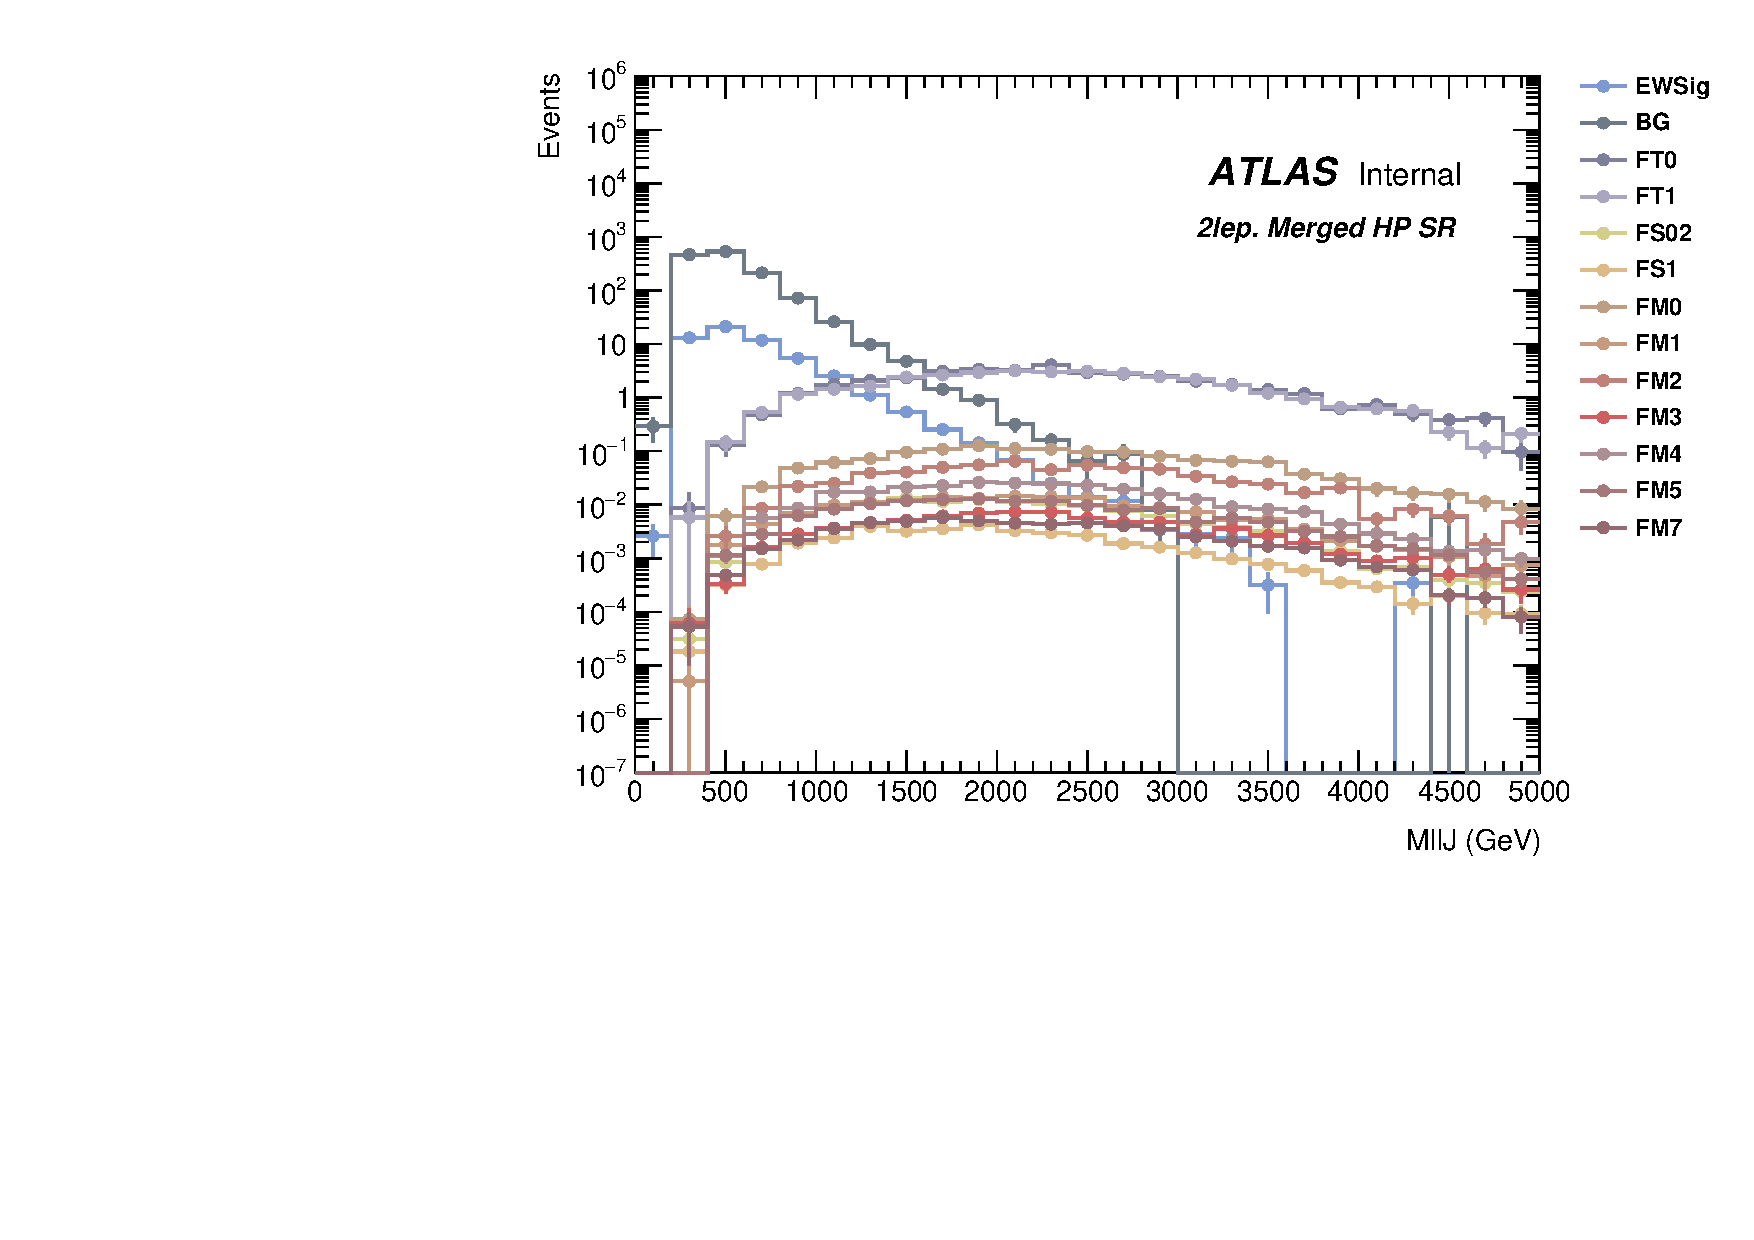
\includegraphics[width=0.45\textwidth]{figures/aQGC/MllJ_SR_HP_aQGC.pdf}
   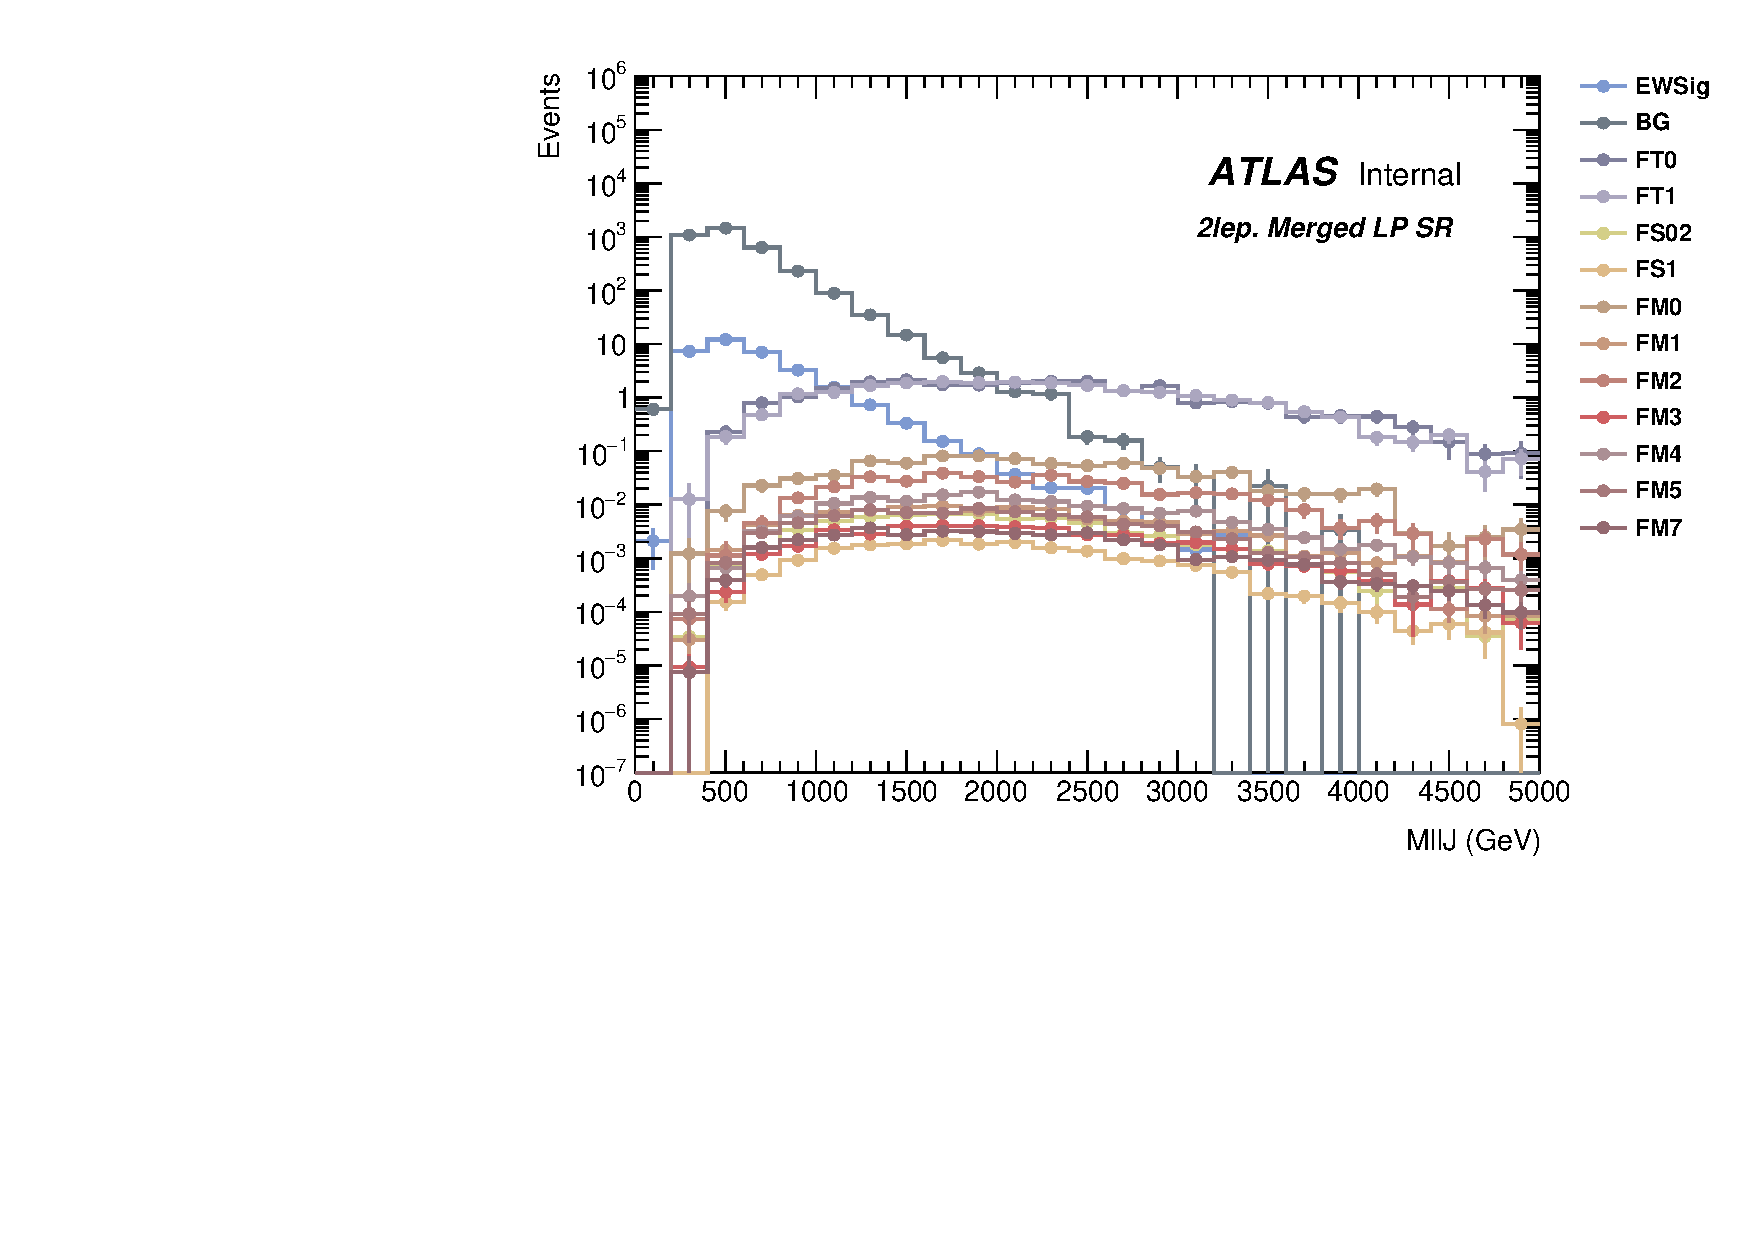
\includegraphics[width=0.45\textwidth]{figures/aQGC/MllJ_SR_LP_aQGC.pdf}
    \caption{$m_{VV}$ shape distribution of each Wilson coefficient in Merged Signal regions. Only quadratic terms are shown.}
    \label{fig:2lepaQGCshapeMVVh}
\end{figure}

\begin{figure}[]
    \centering
   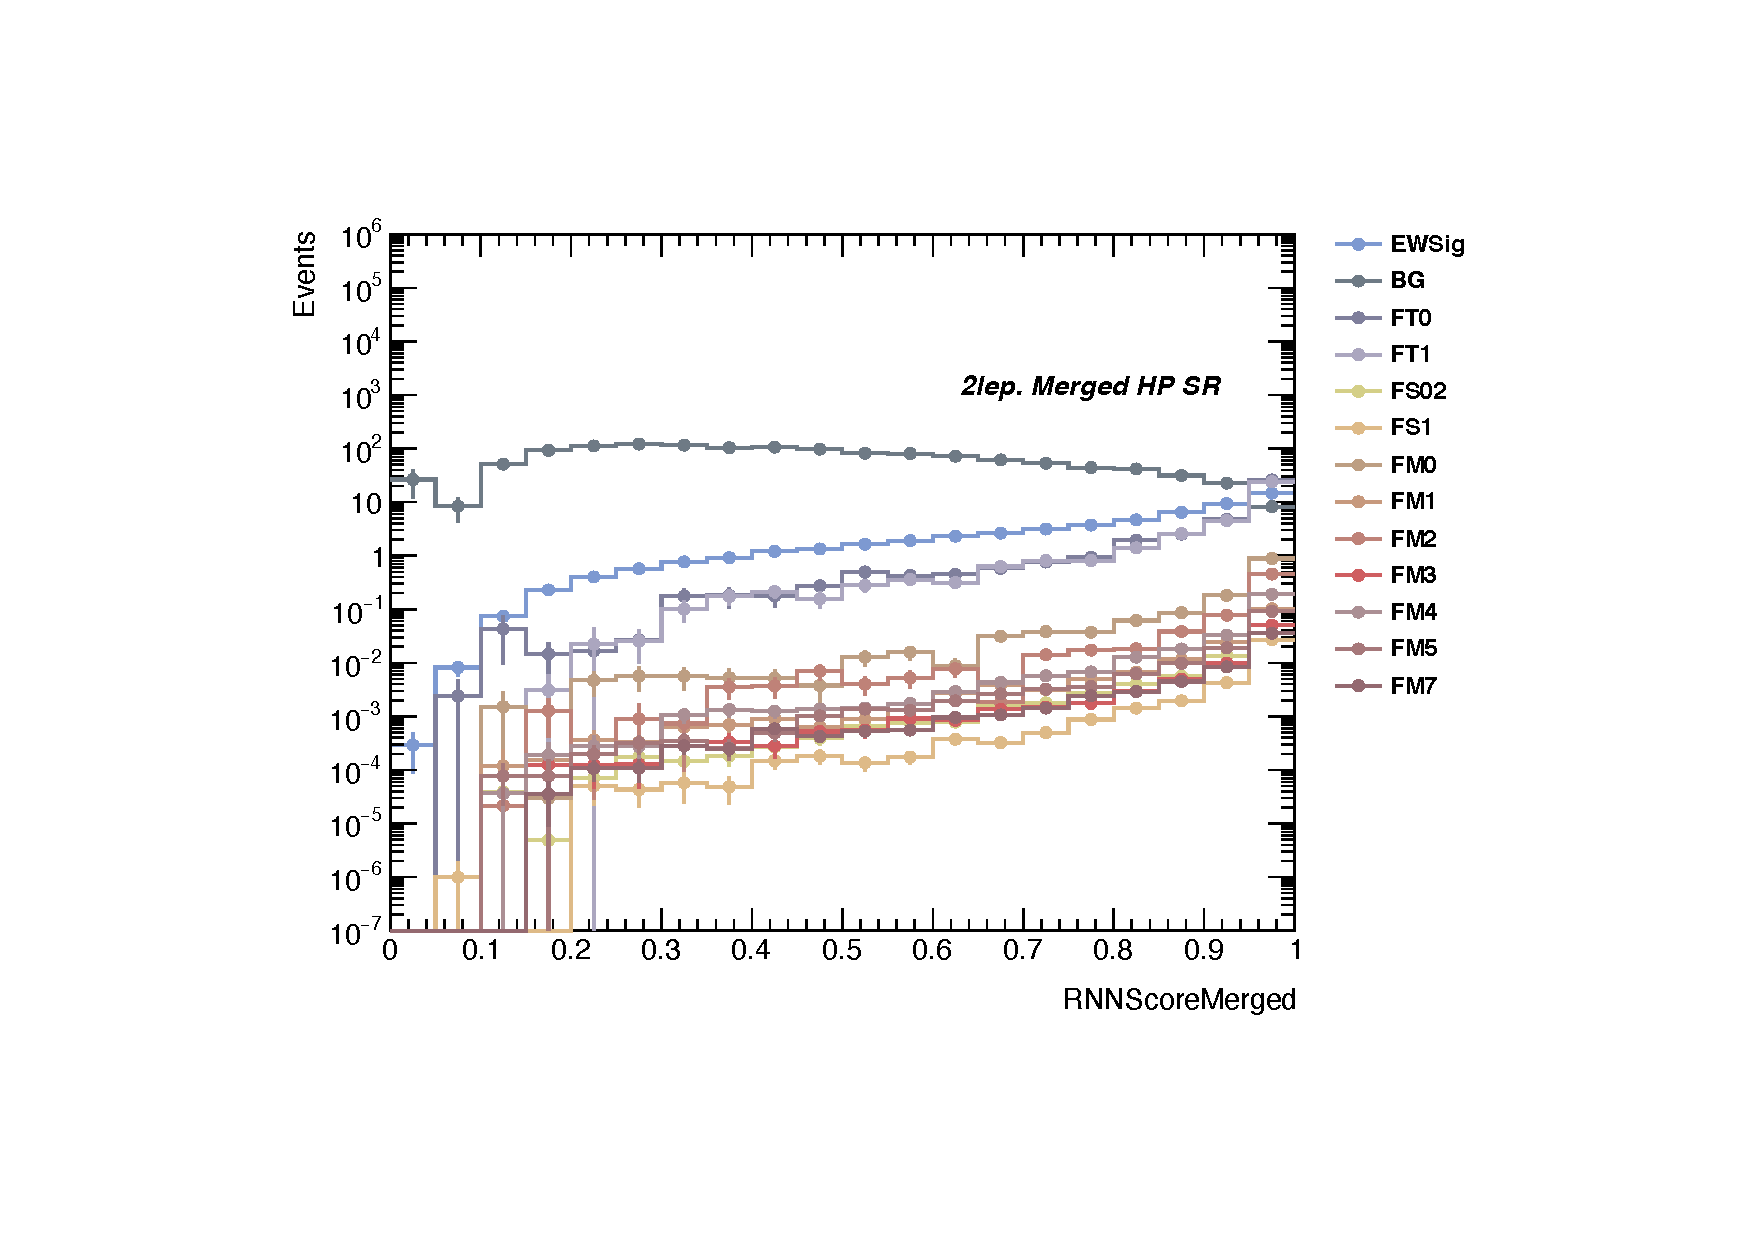
\includegraphics[width=0.45\textwidth]{figures/aQGC/RNNScoreMerged_SR_HP_aQGC.pdf}
   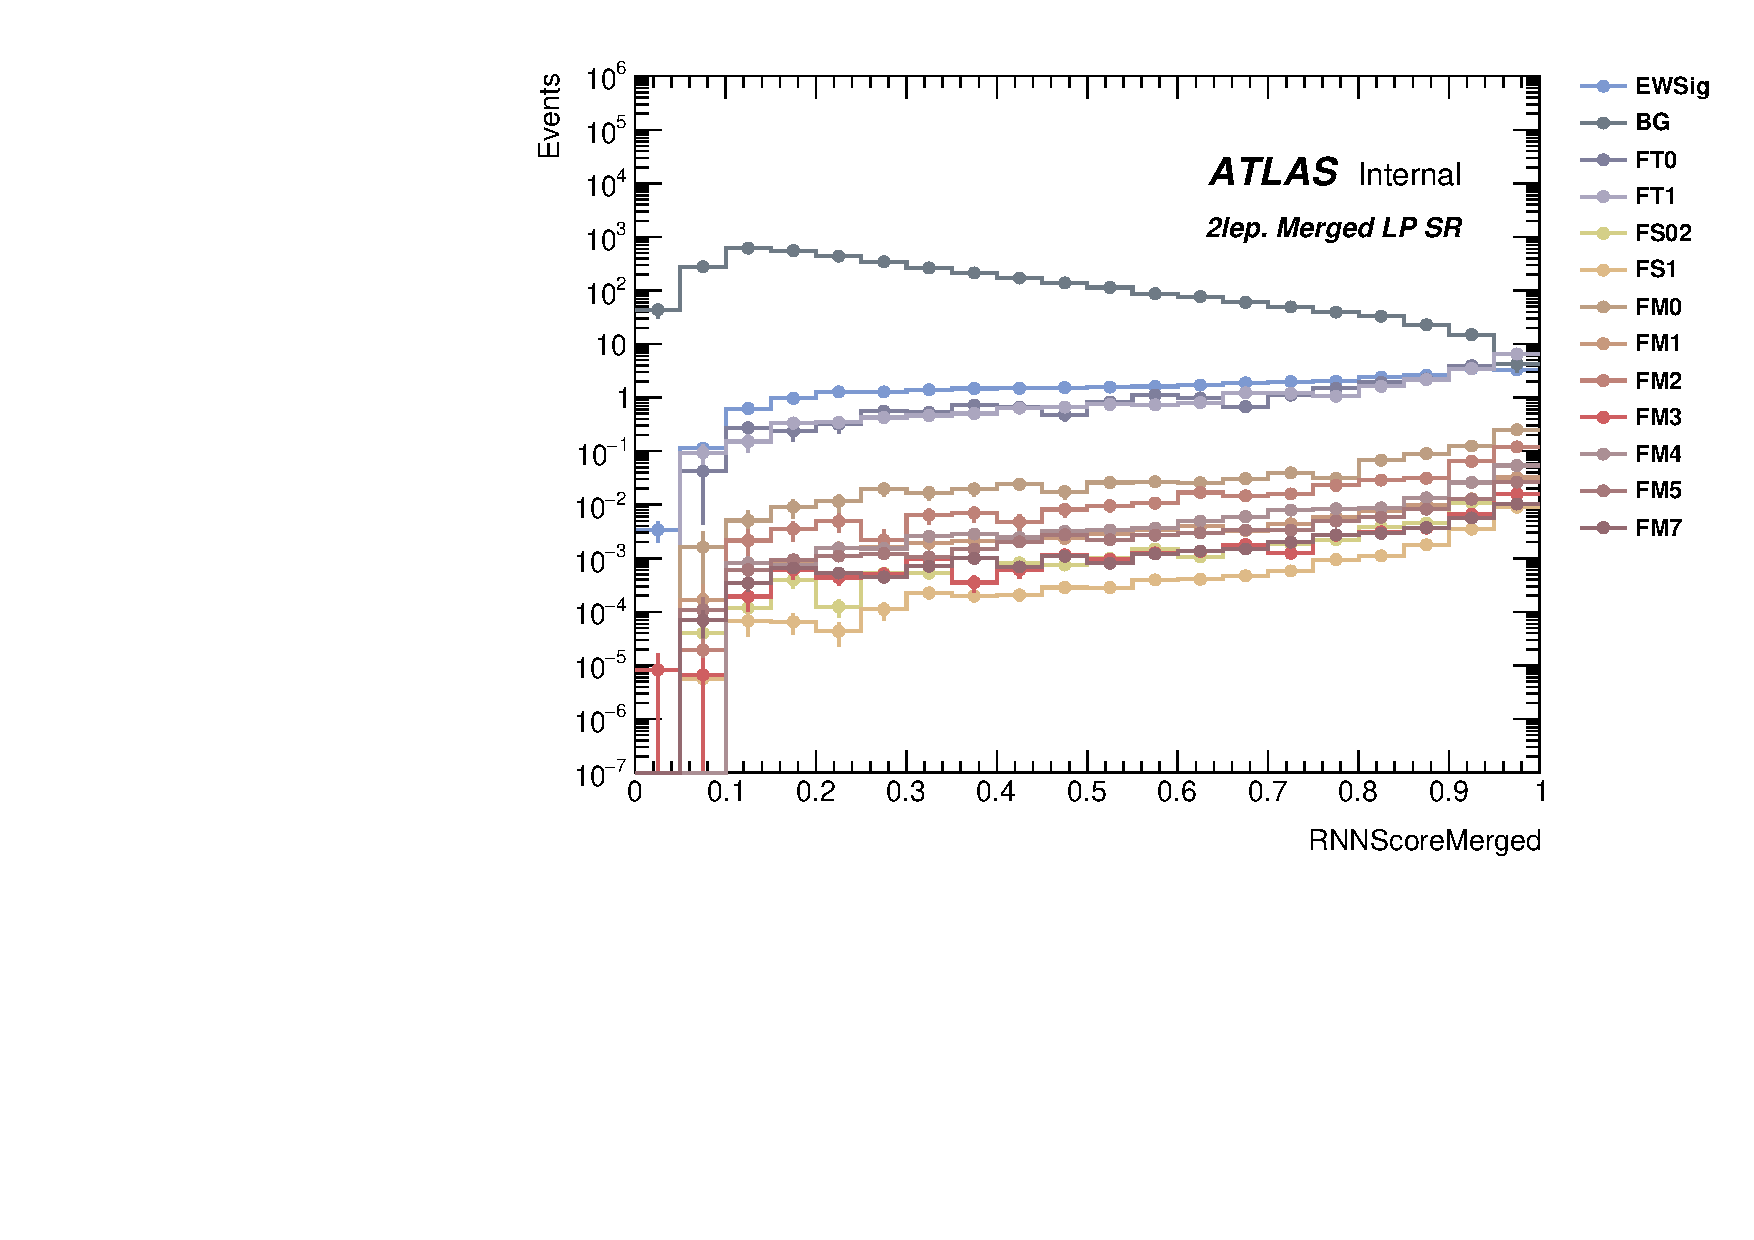
\includegraphics[width=0.45\textwidth]{figures/aQGC/RNNScoreMerged_SR_LP_aQGC.pdf}
    \caption{RNN score shape distribution of each Wilson coefficient in Merged Signal regions. Only quadratic terms are shown.}
    \label{fig:2lepaQGCshapeRNNh}
\end{figure}
%Two-dimensional binning of $m_{VV}$ and the RNN score is used as the final discriminant for the aQGC search.
%In this section, the optimal binning strategy is studied in \tlep\ channel.
%To confirm the result in Section~\ref{subsec:binnedsig} with more realistic setting,

Finally, we would like to separate aQGC signals from both SM electroweak signal and the SM non-VBS background.
So that the final discriminant can make use of the both separation power of $m_{VV}$ and the RNN score, the following study has been performed.

%we compared the results with the following conditions.
The fitting results with the following conditions are compared:
\begin{itemize}
  \item A fit to $m_{VV}$ distribution as discriminant, without any cuts on the RNN score;
  \item A fit to the RNN score distributions after
        SRs are further separated into two subcategories: \\
        Low $m_{VV}$ : $m_{VV}$ $< 2000$~GeV and \\
        High $m_{VV}$ : $m_{VV}$ $\geq 2000$~GeV. \\
\end{itemize}
The threshold 2000~GeV is derived from figure~\ref{fig:2lepaQGCshapeMVVh}.
With the second option, the number of SRs is twice as shown in Figure~\ref{fig:2lepTwoBin}.
%(binning??)
Unconditional asimov fit (The log-likelihood fit using asimov dataset without fixing the $\mu$ value) by using FT0 signal in only \tlep\ channel is performed.
Still, only quadratic term is used in this study.
The systematic uncertainties are not included in the fitting here, just the floated normalization factor is considered.
The asimov data used here is constructed from the background plus SM electroweak VV+jj signal samples.
The expected limits and uncertainty of the expected signal strength of FT0 signal are shown in table~\ref{tab:2binlimit}.
%Significantly better upper limit on the signal strength is obtained by the second option (a fit to RNN score with the categorization by $m_{VV}$)
%than the first option (a fit to $m_{VV}$ distribution).
The signal strength obtained by the second option (a fit to RNN score with the categorization by $m_{VV}$) and the first option (a fit to $m_{VV}$ distribution) is the same. 
We found the first option cannot give any constraints on the SM electroweak VV+jj signal.
It can be a motivation to use the RNN score also in the aQGC search study.

\begin{figure}[ht]
    \centering
    	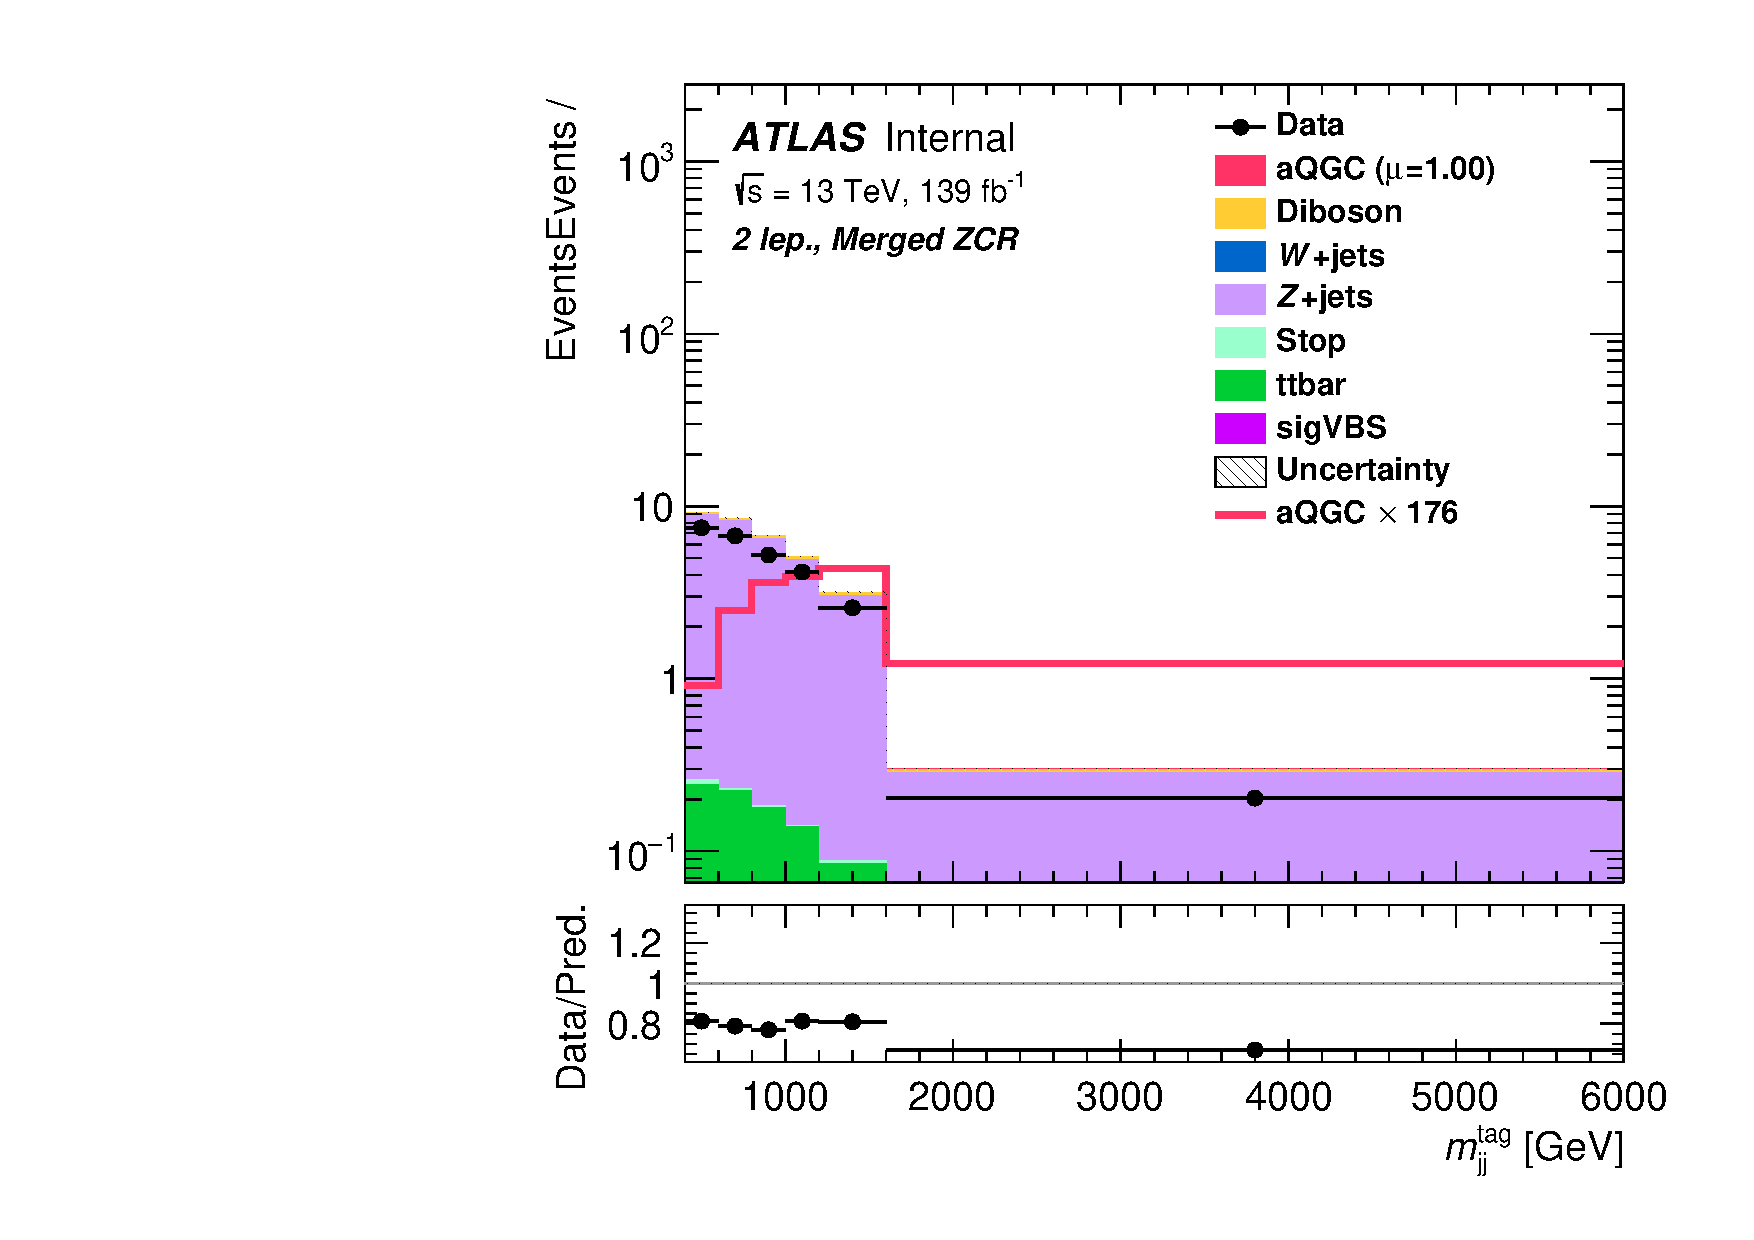
\includegraphics[width=0.32\textwidth]{figures/aQGC/Region_distMTagMerJets_DCRVjet_BMin0_J0_incJet1_L2_T0_incFat1_Y6051_incTag1_Fat1_Prefitlog.pdf}
    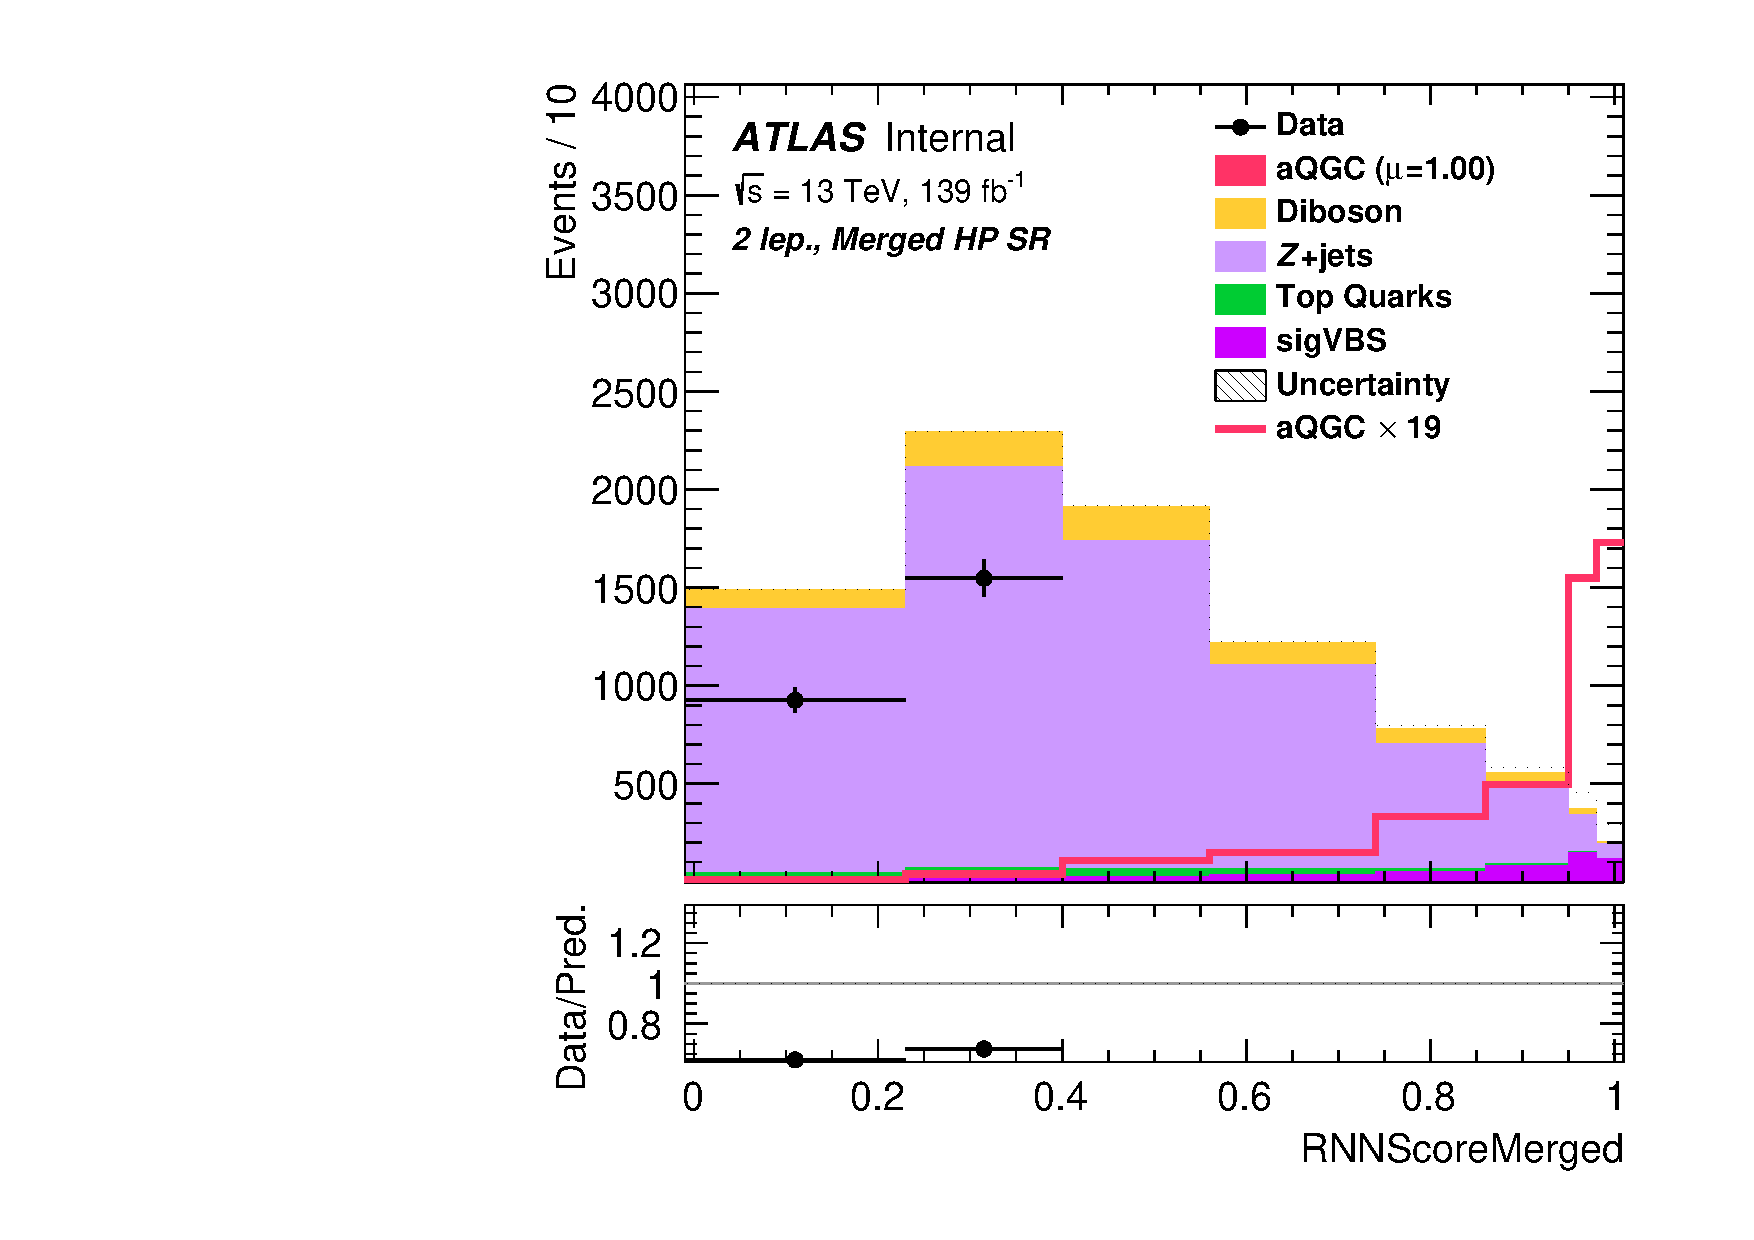
\includegraphics[width=0.32\textwidth]{figures/aQGC/Region_distRNNScoreMerged_DSRVBSHPLMVV_BMin0_J0_incJet1_L2_T0_incFat1_Y6051_incTag1_Fat1_Prefit.pdf}
 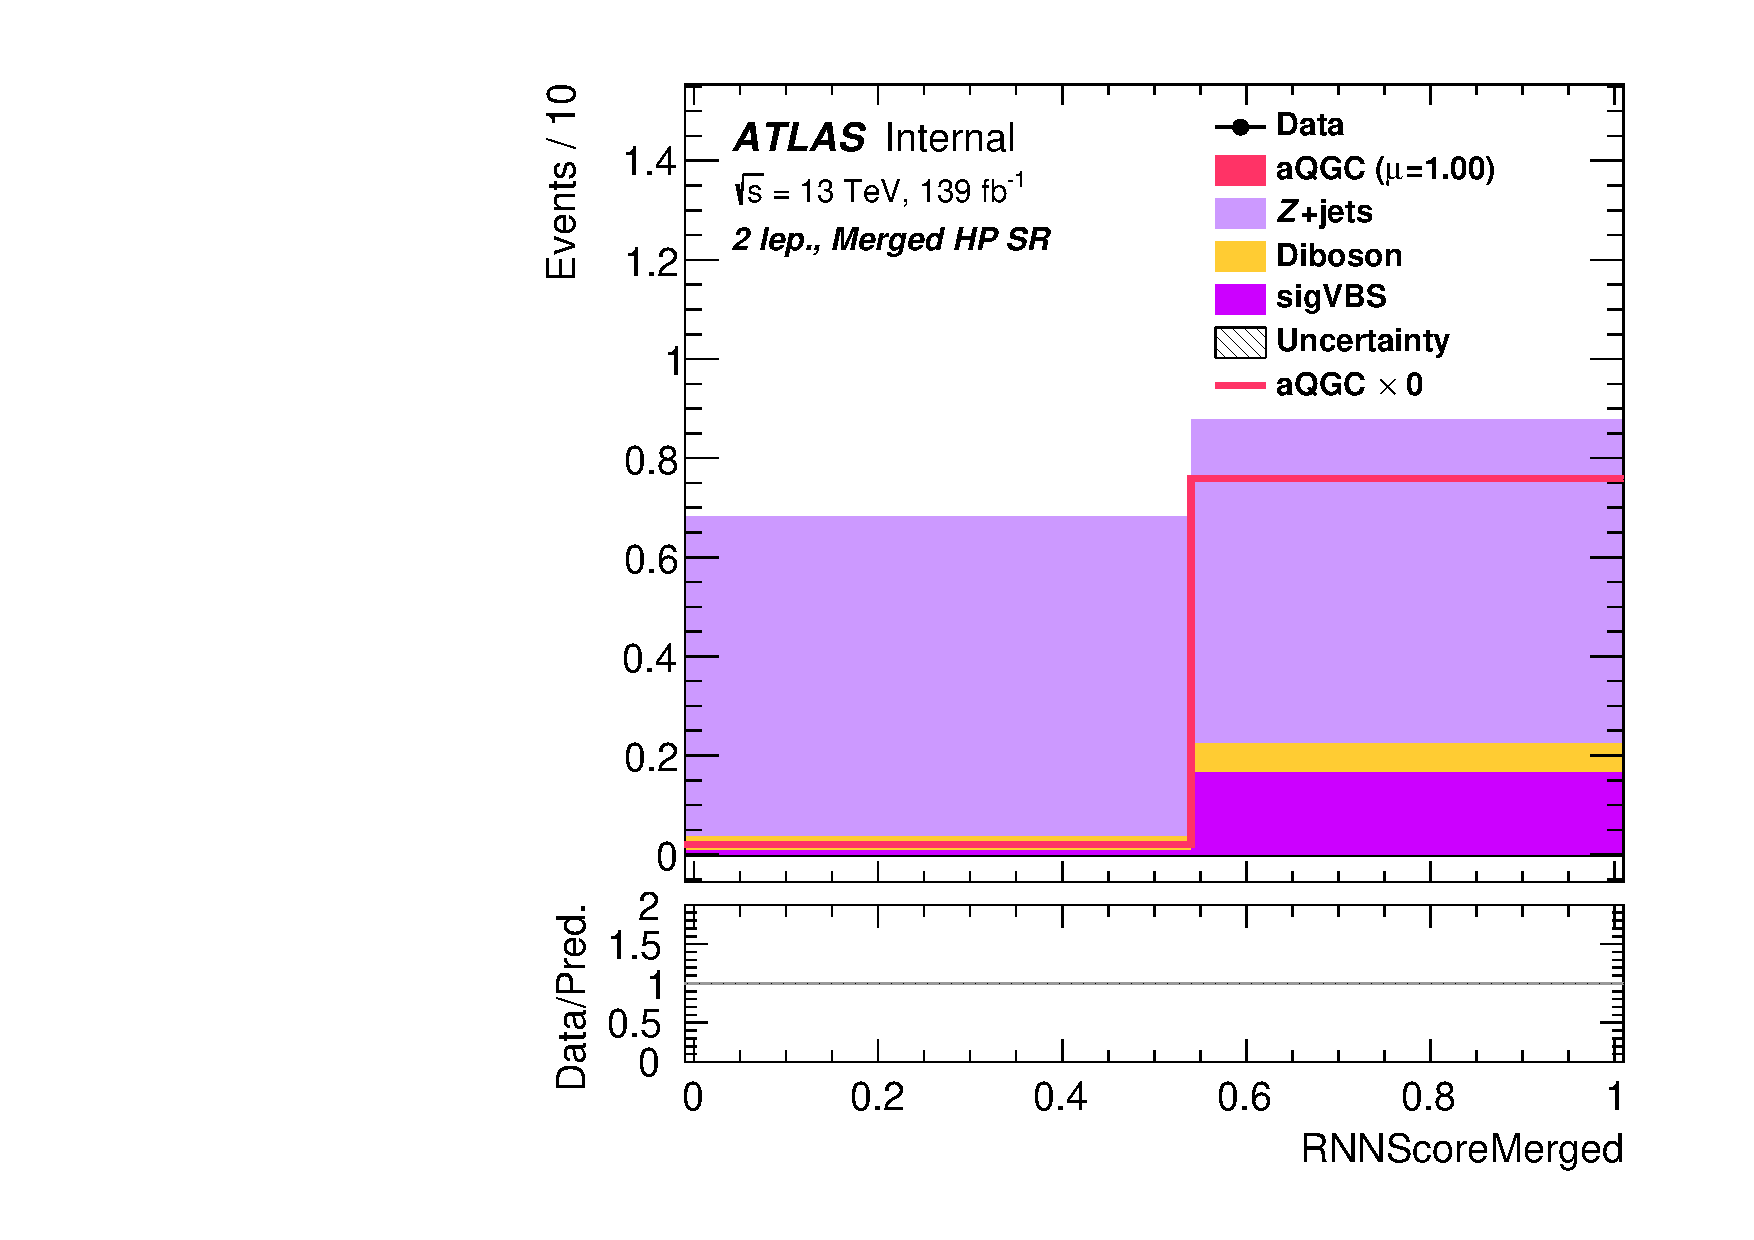
\includegraphics[width=0.32\textwidth]{figures/aQGC/Region_distRNNScoreMerged_DSRVBSHPHMVV_BMin0_J0_incJet1_L2_T0_incFat1_Y6051_incTag1_Fat1_Prefit.pdf}
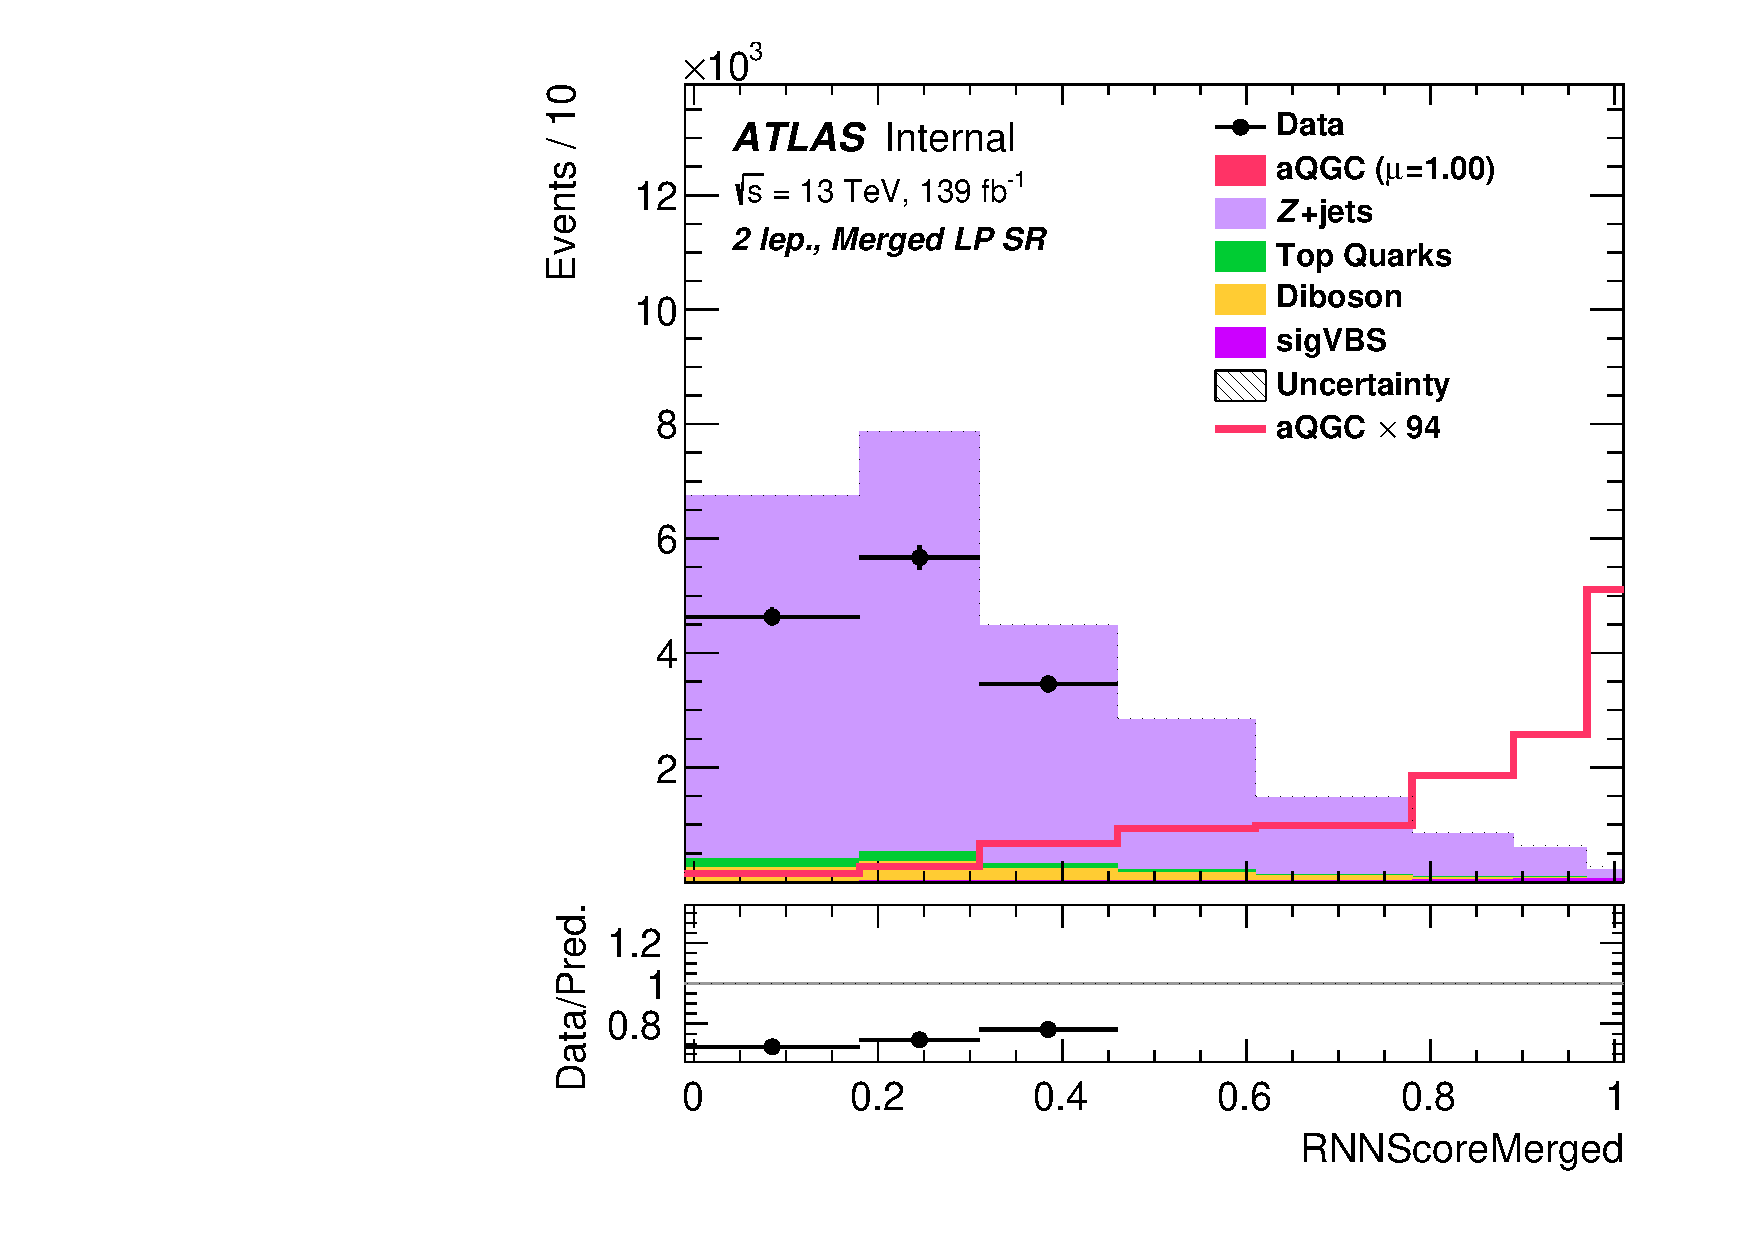
\includegraphics[width=0.32\textwidth]{figures/aQGC/Region_distRNNScoreMerged_DSRVBSLPLMVV_BMin0_J0_incJet1_L2_T0_incFat1_Y6051_incTag1_Fat1_Prefit.pdf}
    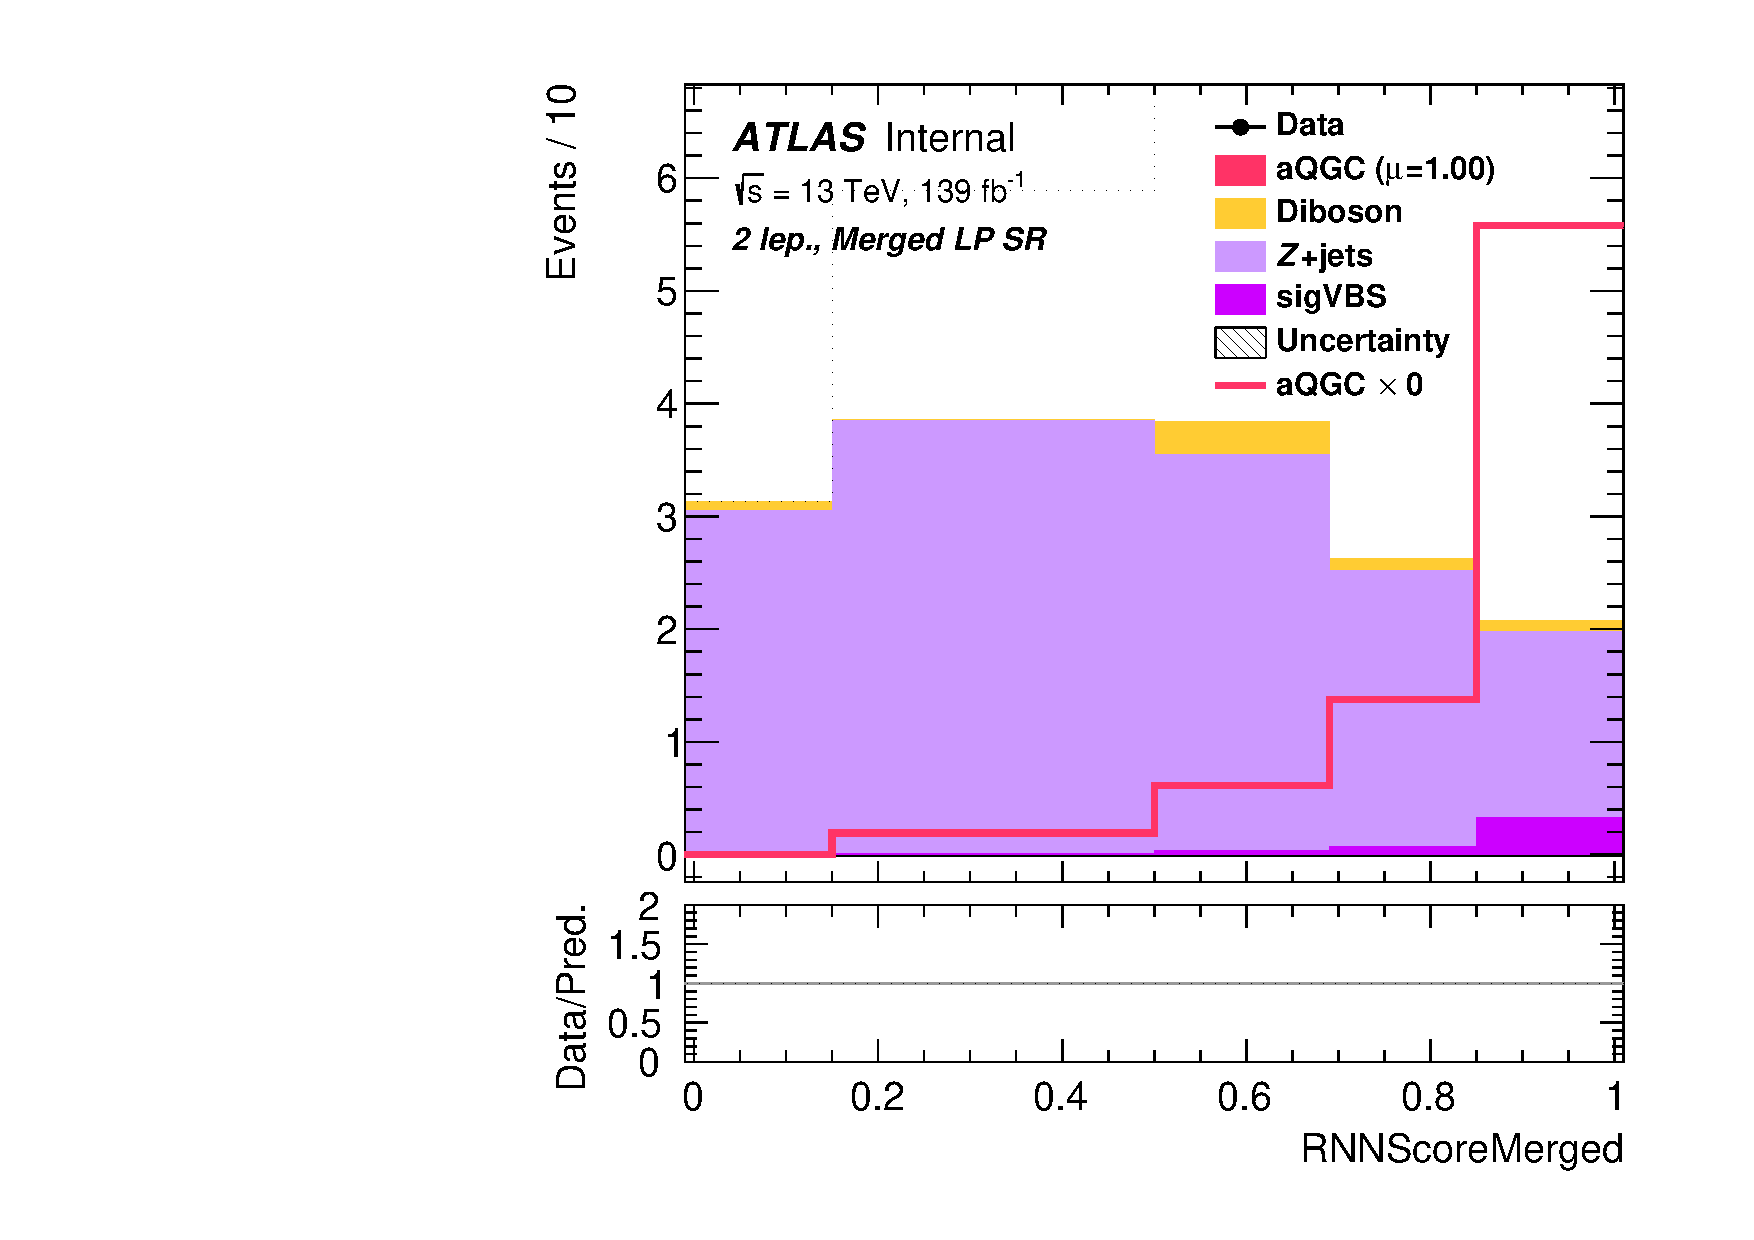
\includegraphics[width=0.32\textwidth]{figures/aQGC/Region_distRNNScoreMerged_DSRVBSLPHMVV_BMin0_J0_incJet1_L2_T0_incFat1_Y6051_incTag1_Fat1_Prefit.pdf}
        \caption{Prefit plots for 2-bin strategy are shown. The RNN score is used as a discriminant for signal regions. operator FT0 in \tlep\ channel are shown. The standard model EW signal is floated as the background.}
        \label{fig:2lepTwoBin}
\end{figure}

%\begin{table}[ht!]
%\small
%\begin{center}
%\resizebox{0.9\textwidth}{!}{
%\begin{tabular}{ | l || l | l | l |}
%\hline
%                                    & Fit to $m_{VV}$ w/o further categorization & Fit to RNN score w/o further categorization  & Fit to RNN scores in separated bins of low- and high-$m_{VV}$  \tabularnewline \hline
%Unconditional fitted $\mu$          & -2.7e-06 $\pm$ 0.067   & 3.38e-05 $\pm0.038$      & 3.35e-05 $\pm0.029$  \tabularnewline \hline
%Norm sigVBS                         & 1 $\pm$ 2.1            & 1 $\pm$ 0.94             & 1 $\pm$ 0.48         \tabularnewline \hline
%Norm Z                              & 1 $\pm$ 0.036          & 1 $\pm$ 0.029            & 1 $\pm$ 0.027        \tabularnewline \hline
%Norm VV                             & 1 $\pm$ 1.13           & 1 $\pm$ 0.71             & 0.99 $\pm$ 0.64      \tabularnewline \hline
%Expected limit of $\mu$             & 0.19                   & 0.72                     & 0.10                 \tabularnewline \hline
%Expected limit of Wilson coefficient & 0.44                   & 0.85                     & 0.32                 \tabularnewline \hline
%\end{tabular}
%}
%\caption{Expected signal strength and limits in every two options. only \tlep channel is used for the fit. The result for single bin fit with RNN is also shown as a reference. The normalization fitted for standard model signal, and Z and diboson backgrounds are shown as Norm in the table.}
%\label{tab:2binlimit}
%\end{center}
%\end{table}

\begin{table}[ht!]
\small
\begin{center}
\resizebox{\textwidth}{!}{
\begin{tabular}{ | l || l | l | l |}
\hline
                                    & Fit to $m_{VV}$ w/o further categorization & Fit to RNN score w/o further categorization  & Fit to RNN scores in separated bins of low- and high-$m_{VV}$  \tabularnewline \hline
Unconditional fitted $\mu$          & 8.83e-06 $\pm0.032$    & 1.02e-04 $\pm0.34$       & 1.09e-05 $\pm0.028$  \tabularnewline \hline
Norm sigVBS                         & 1 $\pm$ 1.08           & 1 $\pm$ 0.79             & 1 $\pm$ 0.41         \tabularnewline \hline
Norm Z                              & 1 $\pm$ 0.012          & 1 $\pm$ 0.010            & 1 $\pm$ 0.01         \tabularnewline \hline
Expected limit of $\mu$             & 0.11                   & 0.70                     & 0.11                 \tabularnewline \hline
Expected limit of Wilson coefficient & 0.33                  & 0.84                     & 0.33                 \tabularnewline \hline
\end{tabular}
}
\caption{Expected signal strength and limits in every two options. only \tlep~channel is used for the fit. The result for single bin fit with RNN is also shown as a reference. The normalization fitted for the standard model signal, and Z backgrounds are shown as Norm in the table.}
\label{tab:2binlimit}
\end{center}
\end{table}

%\section{Optimization of the threshold of 2-bin approach}
%\label{subsec:aQGCbinninb}
Of course, the optimal threshold of $m_{VV}$ can be different depending on the clipping energy.
In addition, a fine-tuning of the $m_{VV}$ threshold might be needed by considering the stability of the background estimation.
The expected limit is shown in each threshold for $m_{VV}$ of 1000~GeV, 1500~GeV, 2000~GeV for variety of the clipping points in Figure~\ref{fig:ThresholdScan}.

As expected, higher $m_{VV}$ threshold is preferred at the higher clipping point, while lower $m_{VV}$ threshold is favored at the lower clipping point.
1500~GeV is chosen as the best compromise to separate SRs into low- and high-$m_{VV}$ bins.

Since the meaning of the actual $m_{VV}$ distributions used in each lepton channel are different
(fully reconstructed system in \tlep\ and in \olep\ (solving neutrino ambiguity) and transverse mass in \zlep\)
the optimal thresholds to separate SRs into low- and high-$m_{VV}$ bins in \olep\ and \zlep\ channels 
are determined as follows.
In \olep\ channel, the same threshold as \tlep\ channel, 1500~GeV, is just chosen since the reconstructed $m_{VV}$ distribution is similar. 
%(?)
In \zlep\ channel, the threshold needs to be optimized, since it uses \mt\ instead of $m_{VV}$.
As shown in Figure~\ref{fig:mVVdist} the \mt\ shape in \zlep\ channel is different from $m_{VV}$ in \tlep\ channel.
Here, the background yield in each bin of the high-$\mt$ regions is adjusted to be more than 5 so that
the asymptotic calculation of the sensitivity is ensured with a certain number of background events.
The threshold finalized is shown in Table, for each lepton channel, and for each region.

Only in \tlep\ channel,
less than 5 background events are expected in the second bin of the HP signal region.
%We are going to test if the asymptotic formulae works fine, by running toy experiments [TO DO].
%
\begin{figure}[h]
        \centering
    	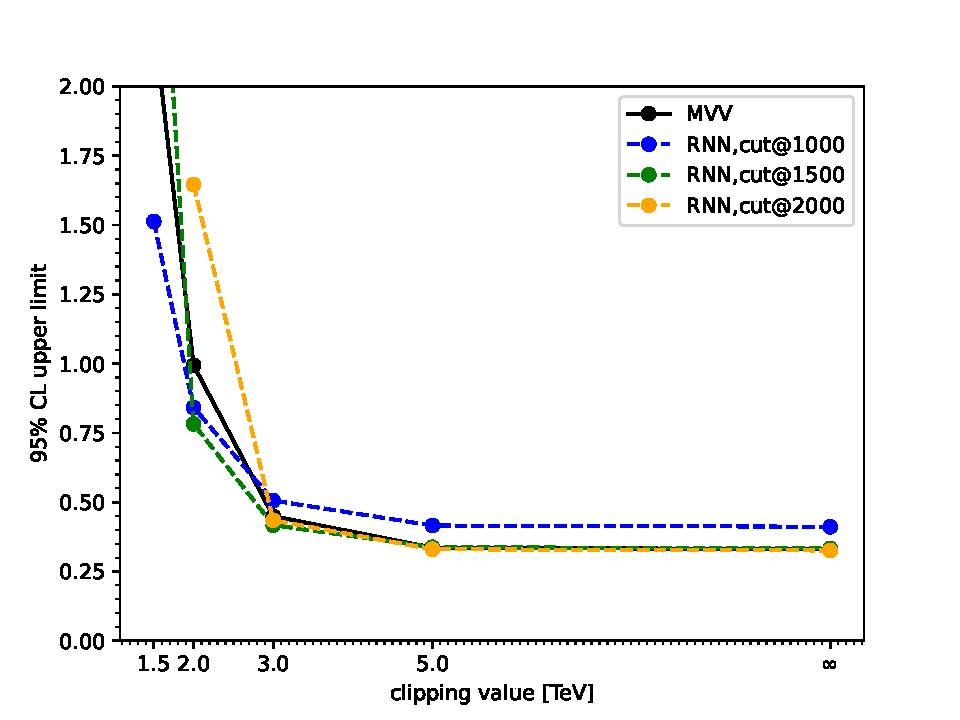
\includegraphics[width=0.50\textwidth]{figures/aQGC/ClippedFT02bin.pdf}
        \caption{Expected limits for 5 clipping points with each threshold for dividing $m_{VV}$ into 2 bins.}
        \label{fig:ThresholdScan}
\end{figure}

\begin{figure}[ht]
    \centering
    	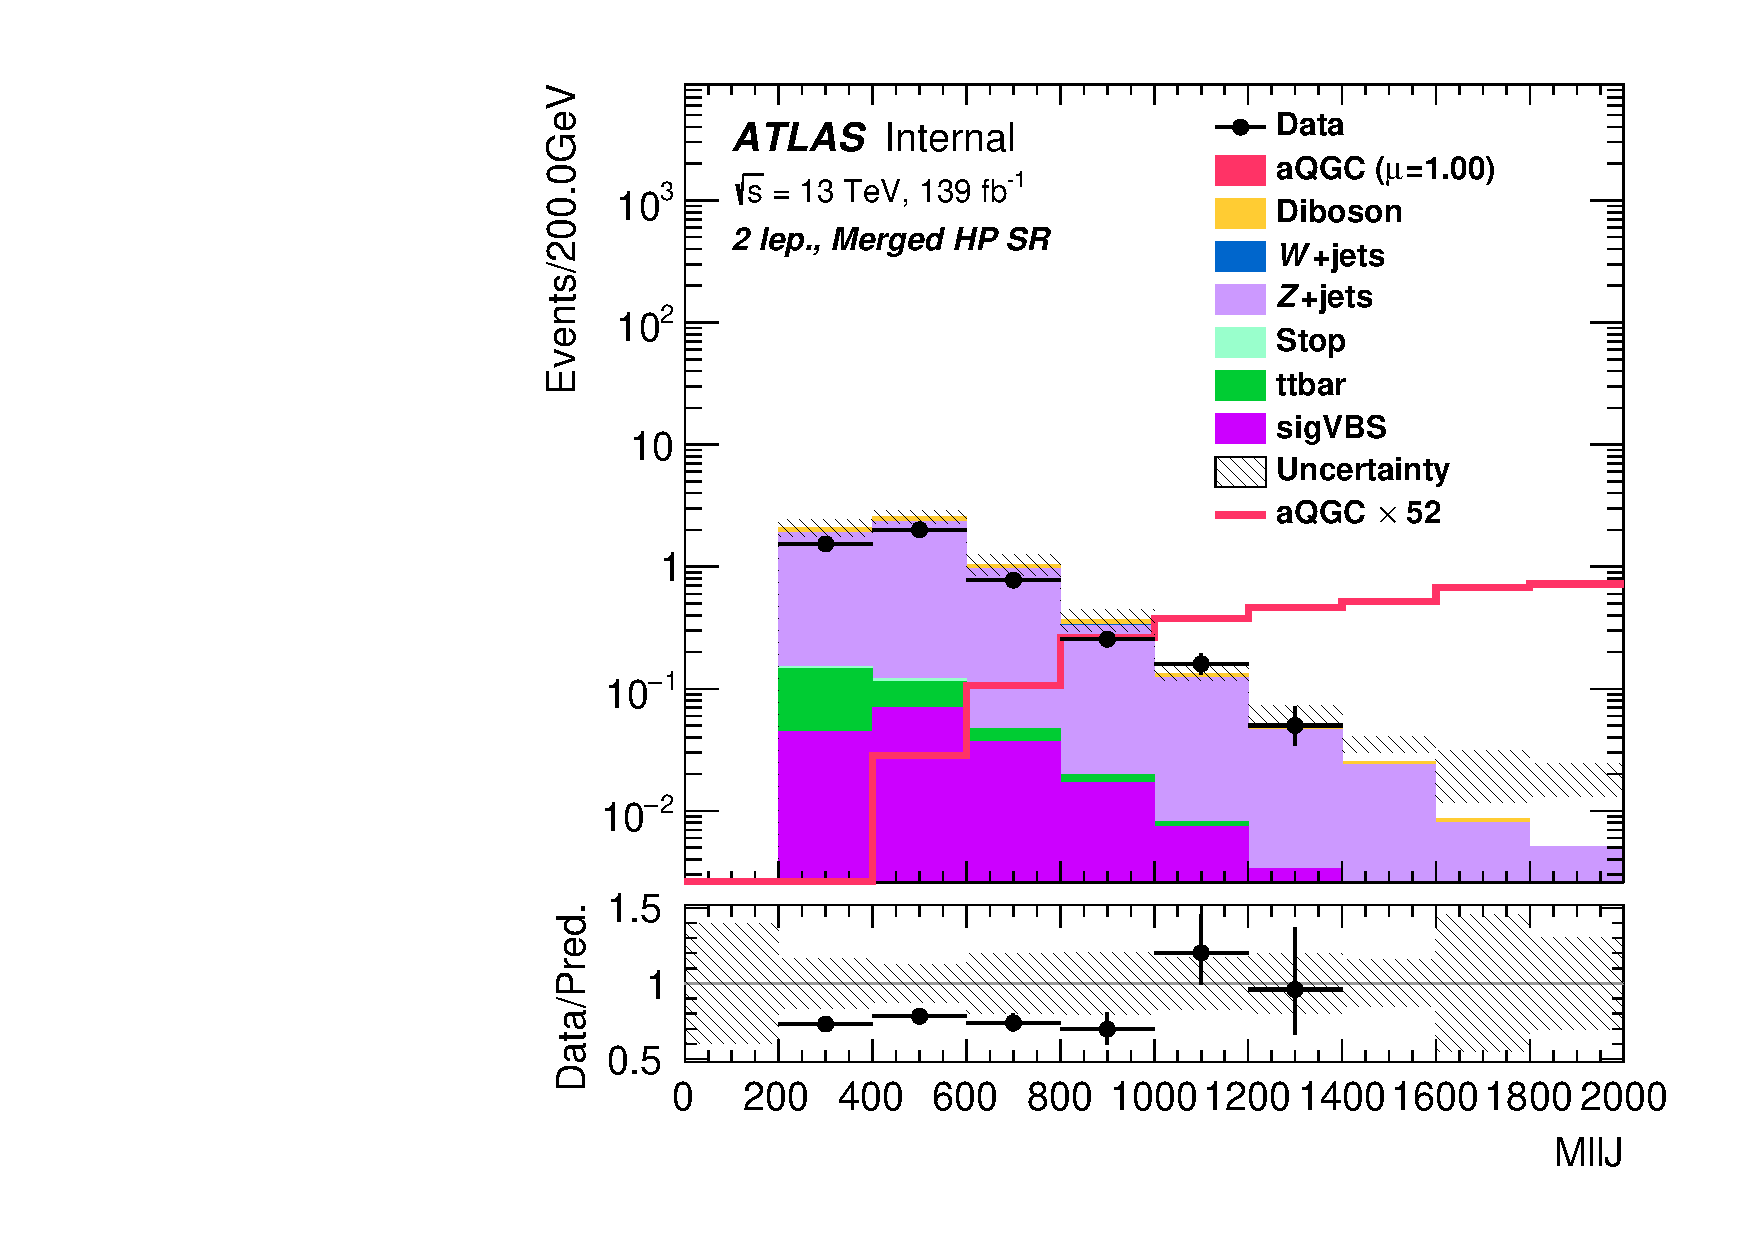
\includegraphics[width=0.32\textwidth]{figures/aQGC/MVV/Region_distMllJ_DSRVBSHP_BMin0_J0_incJet1_L2_T0_incFat1_Y6051_incTag1_Fat1_Prefitlog.pdf}
    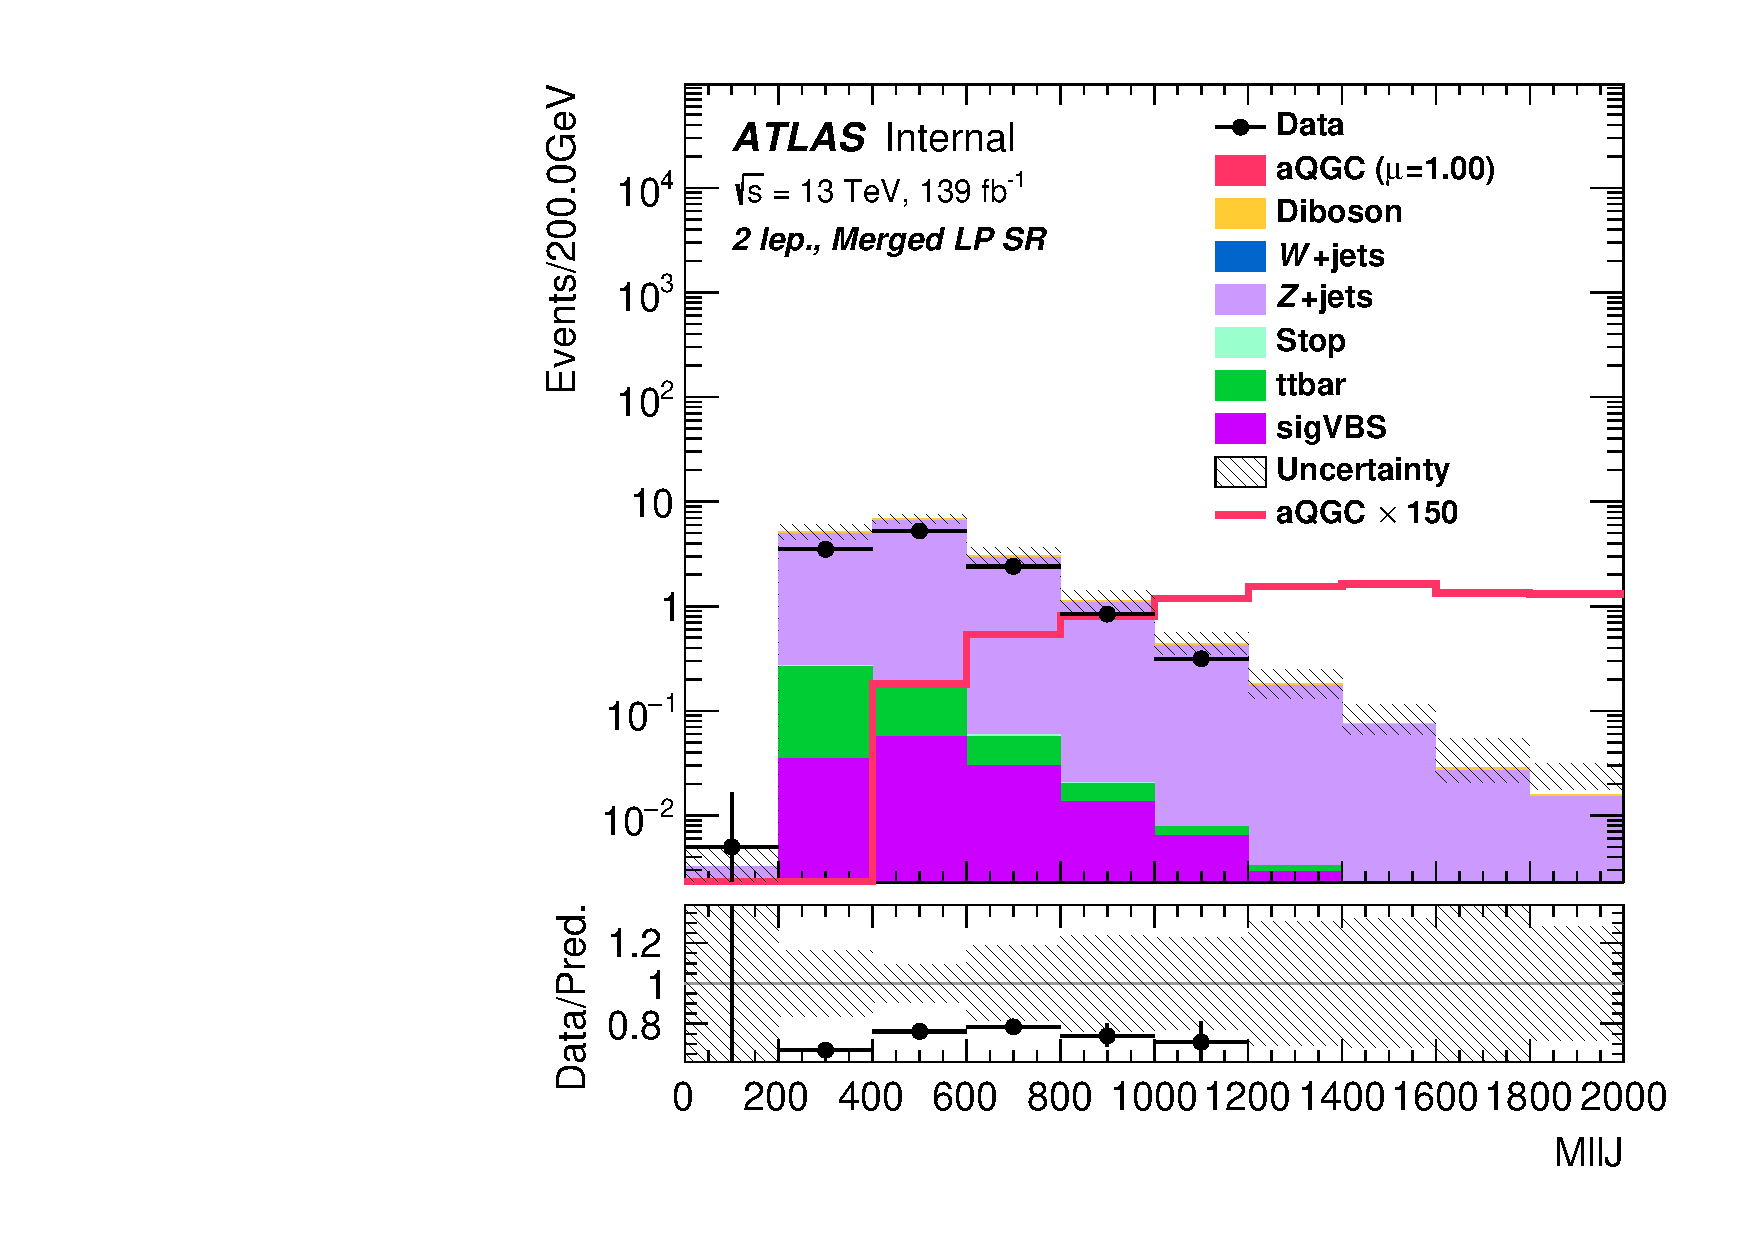
\includegraphics[width=0.32\textwidth]{figures/aQGC/MVV/Region_distMllJ_DSRVBSLP_BMin0_J0_incJet1_L2_T0_incFat1_Y6051_incTag1_Fat1_Prefitlog.pdf}
  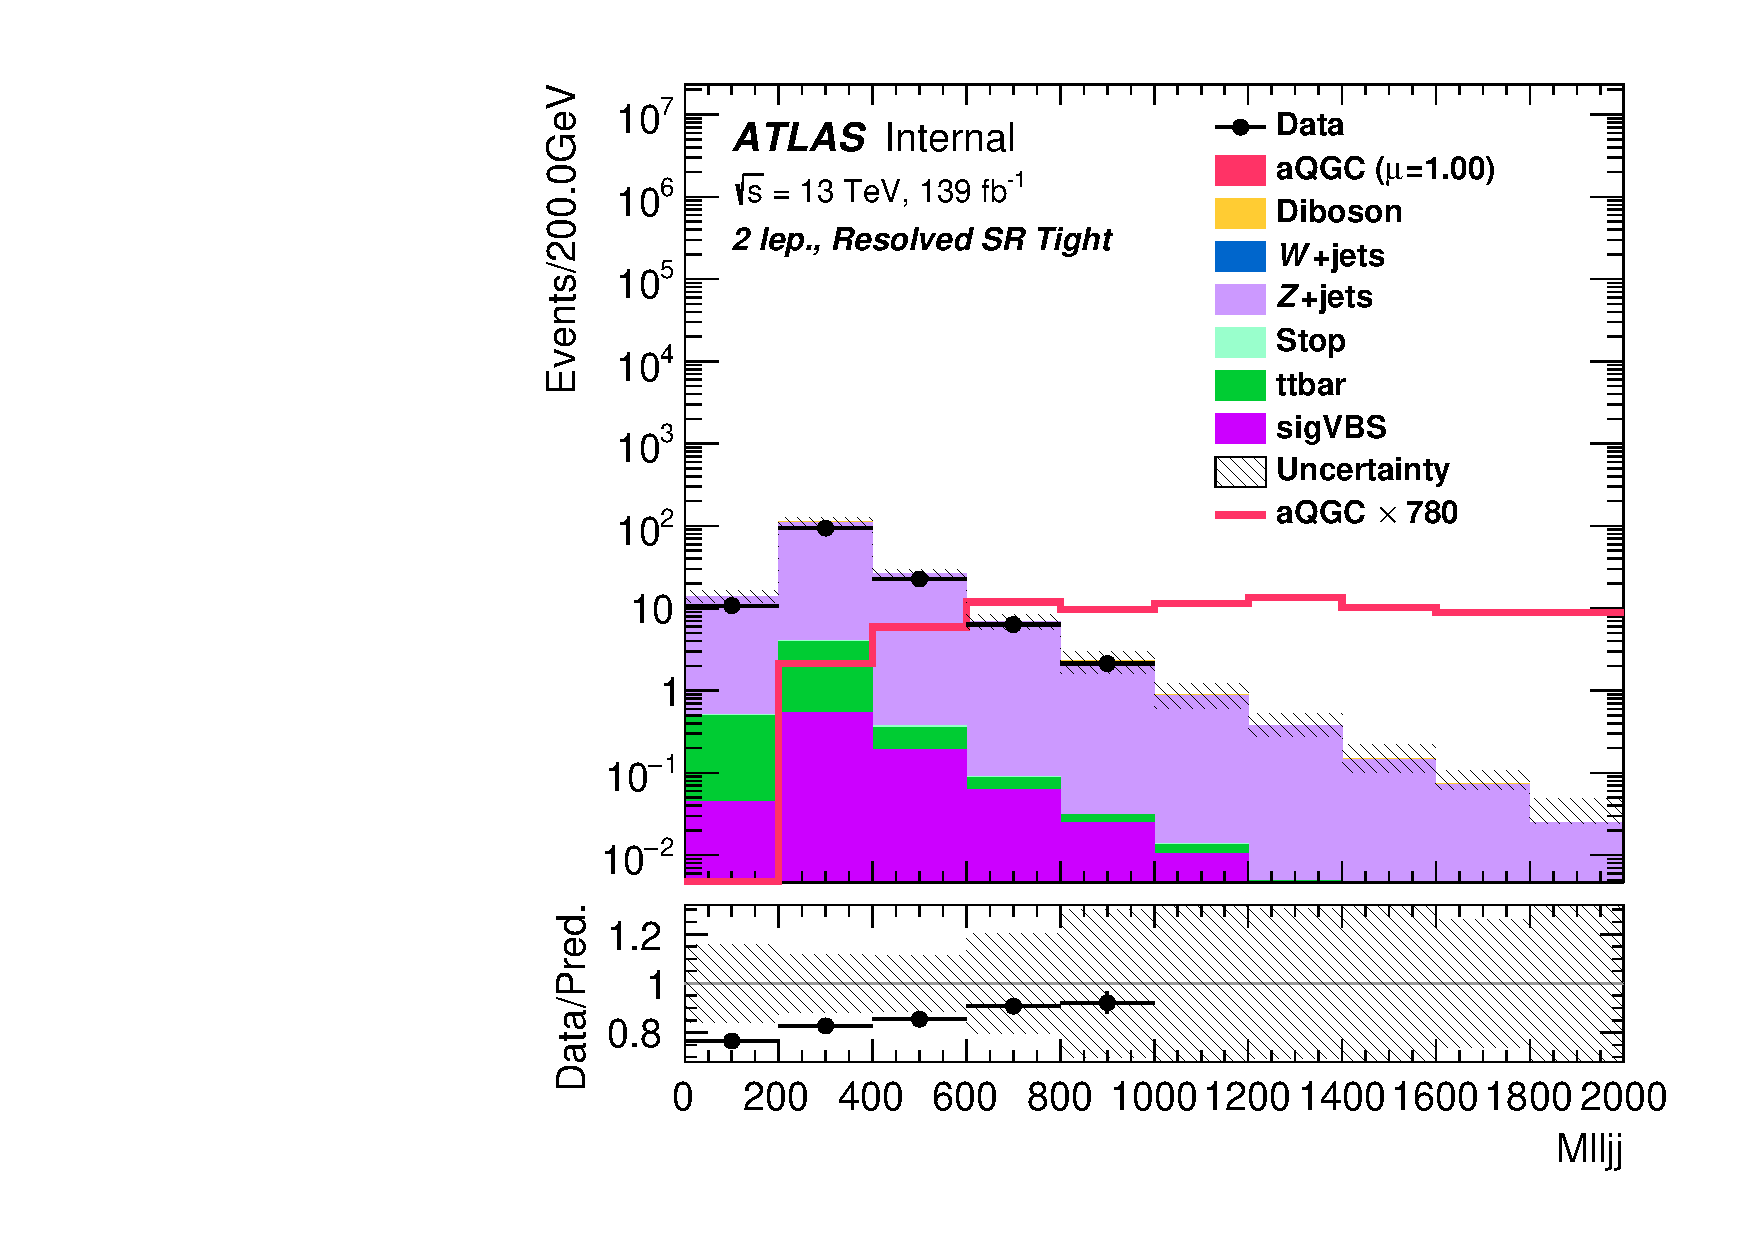
\includegraphics[width=0.32\textwidth]{figures/aQGC/MVV/Region_distMlljj_DSRVBSFid_BMin0_T0_Y6051_incTag1_J2_L2_incJet1_Prefitlog.pdf}
    	%\subfigure[ 1lep HP SR ]{\includegraphics[width=0.32\textwidth]{figures/aQGC/MVV/}}
    	%\subfigure[ 1lep LP SR ]{\includegraphics[width=0.32\textwidth]{figures/aQGC/MVV/}}
    	%\subfigure[ 1lep Fid SR ]{\includegraphics[width=0.32\textwidth]{figures/aQGC/MVV/}}
    	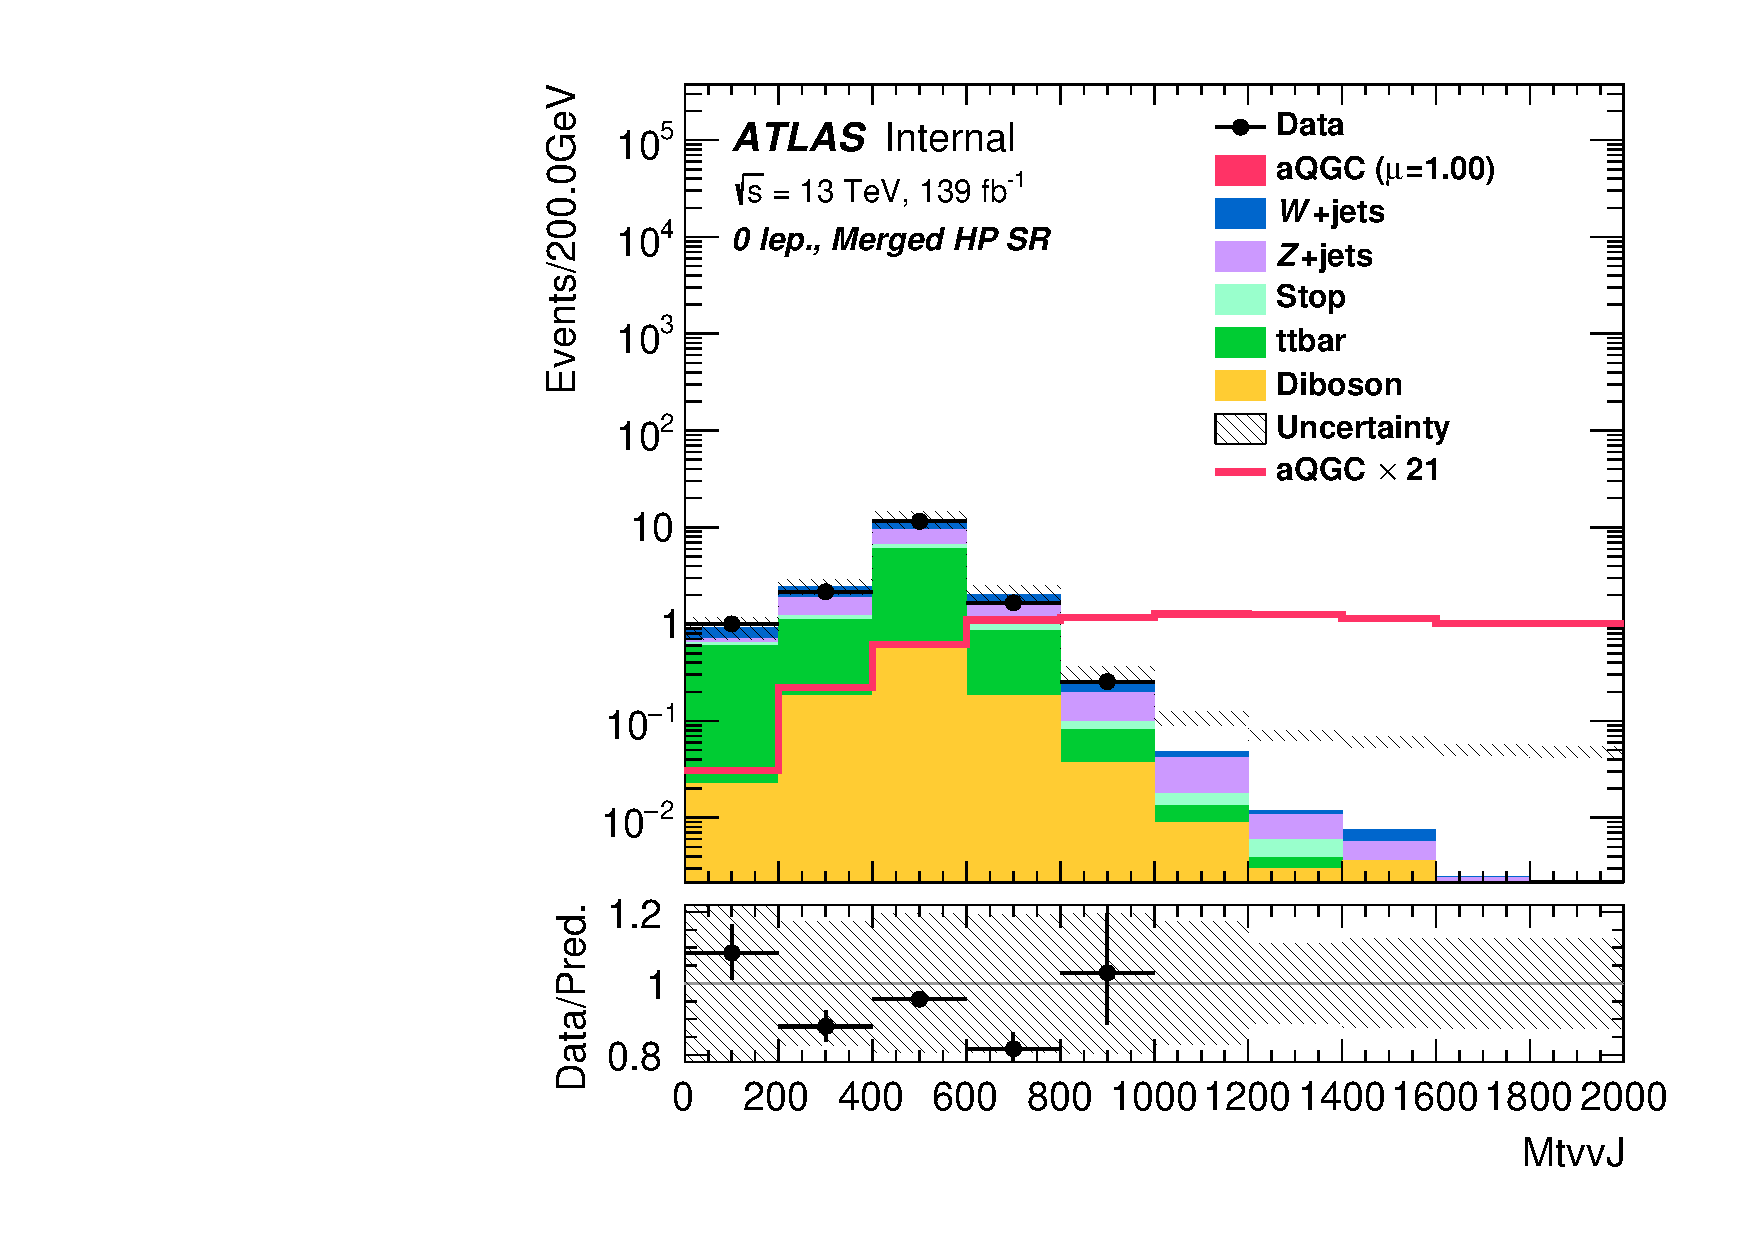
\includegraphics[width=0.32\textwidth]{figures/aQGC/MVV/Region_distMtvvJ_DSRVBSHP_BMin0_J0_incJet1_L0_T0_incFat1_Y6051_incTag1_Fat1_Prefitlog.pdf}
    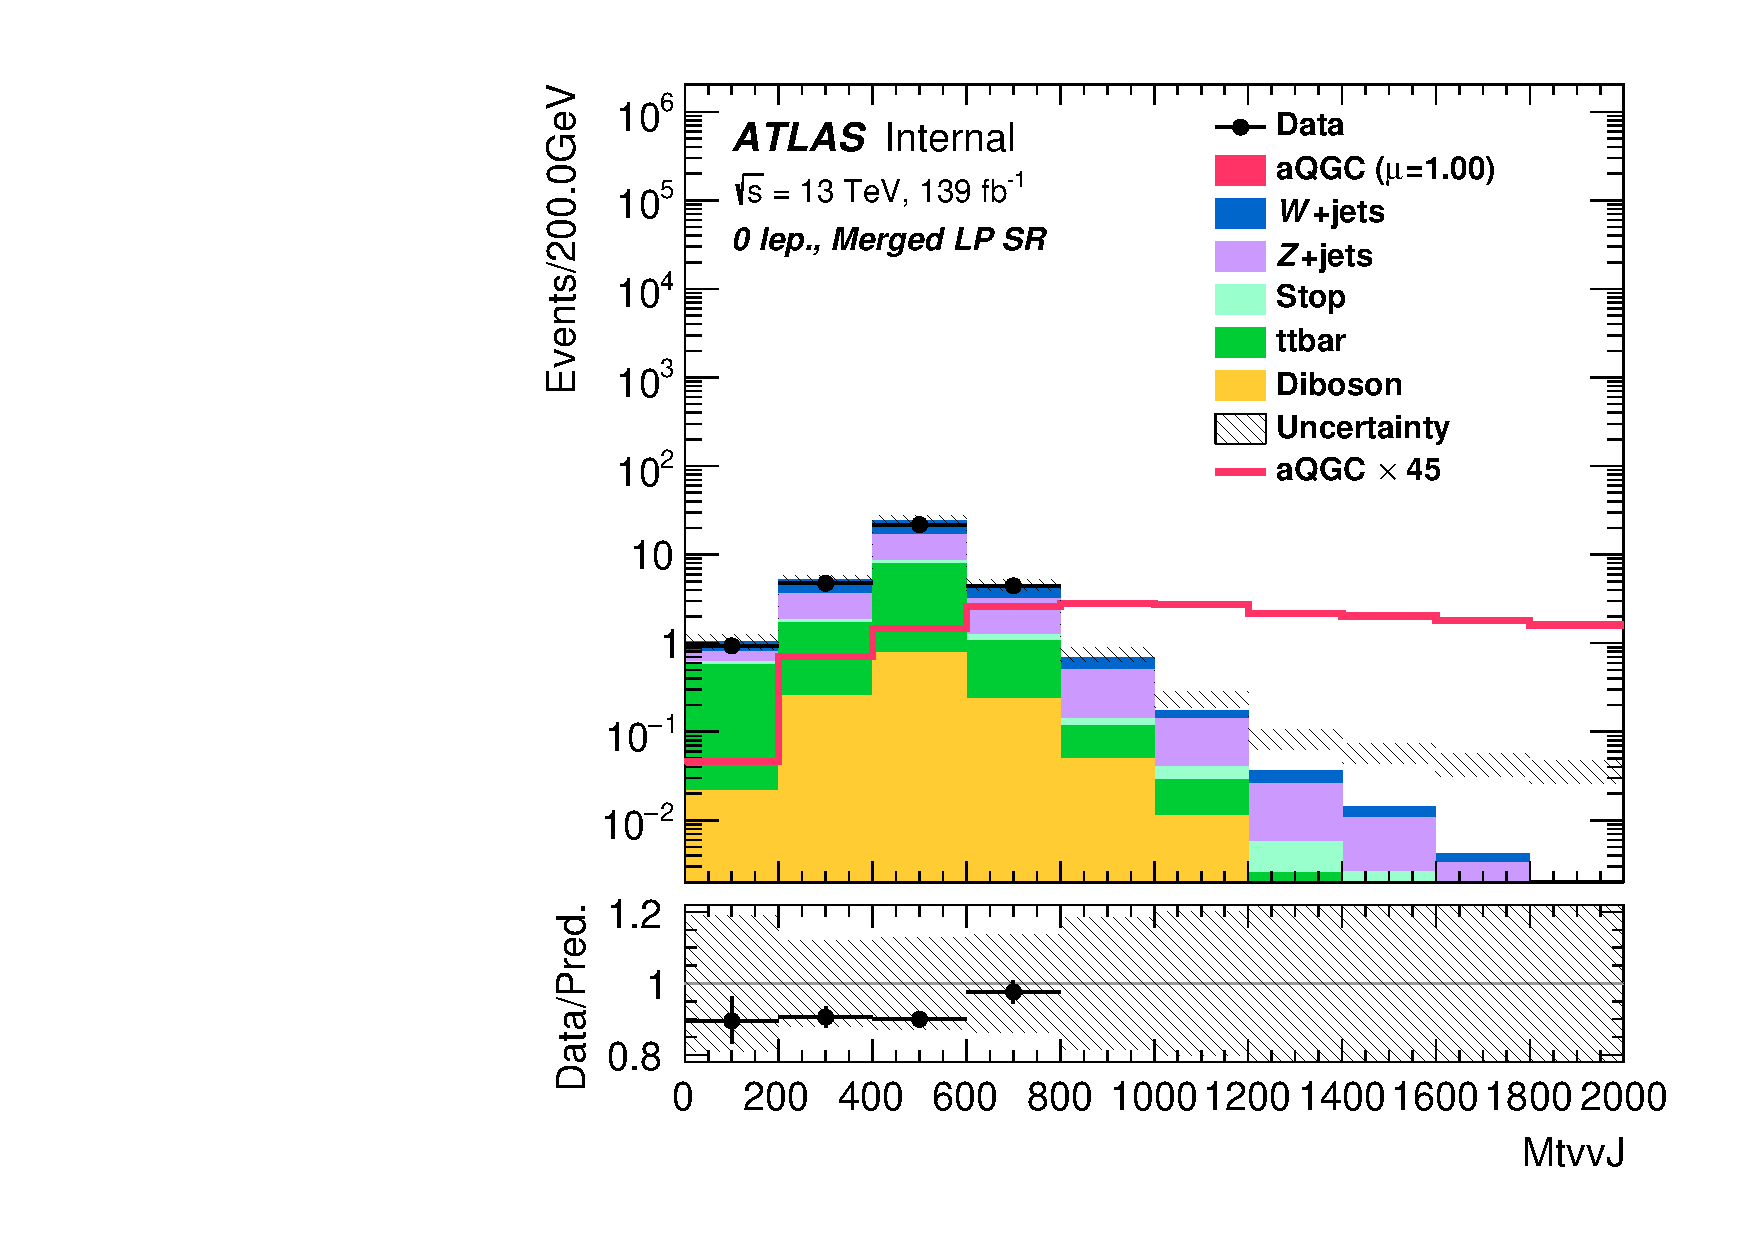
\includegraphics[width=0.32\textwidth]{figures/aQGC/MVV/Region_distMtvvJ_DSRVBSLP_BMin0_J0_incJet1_L0_T0_incFat1_Y6051_incTag1_Fat1_Prefitlog.pdf}
 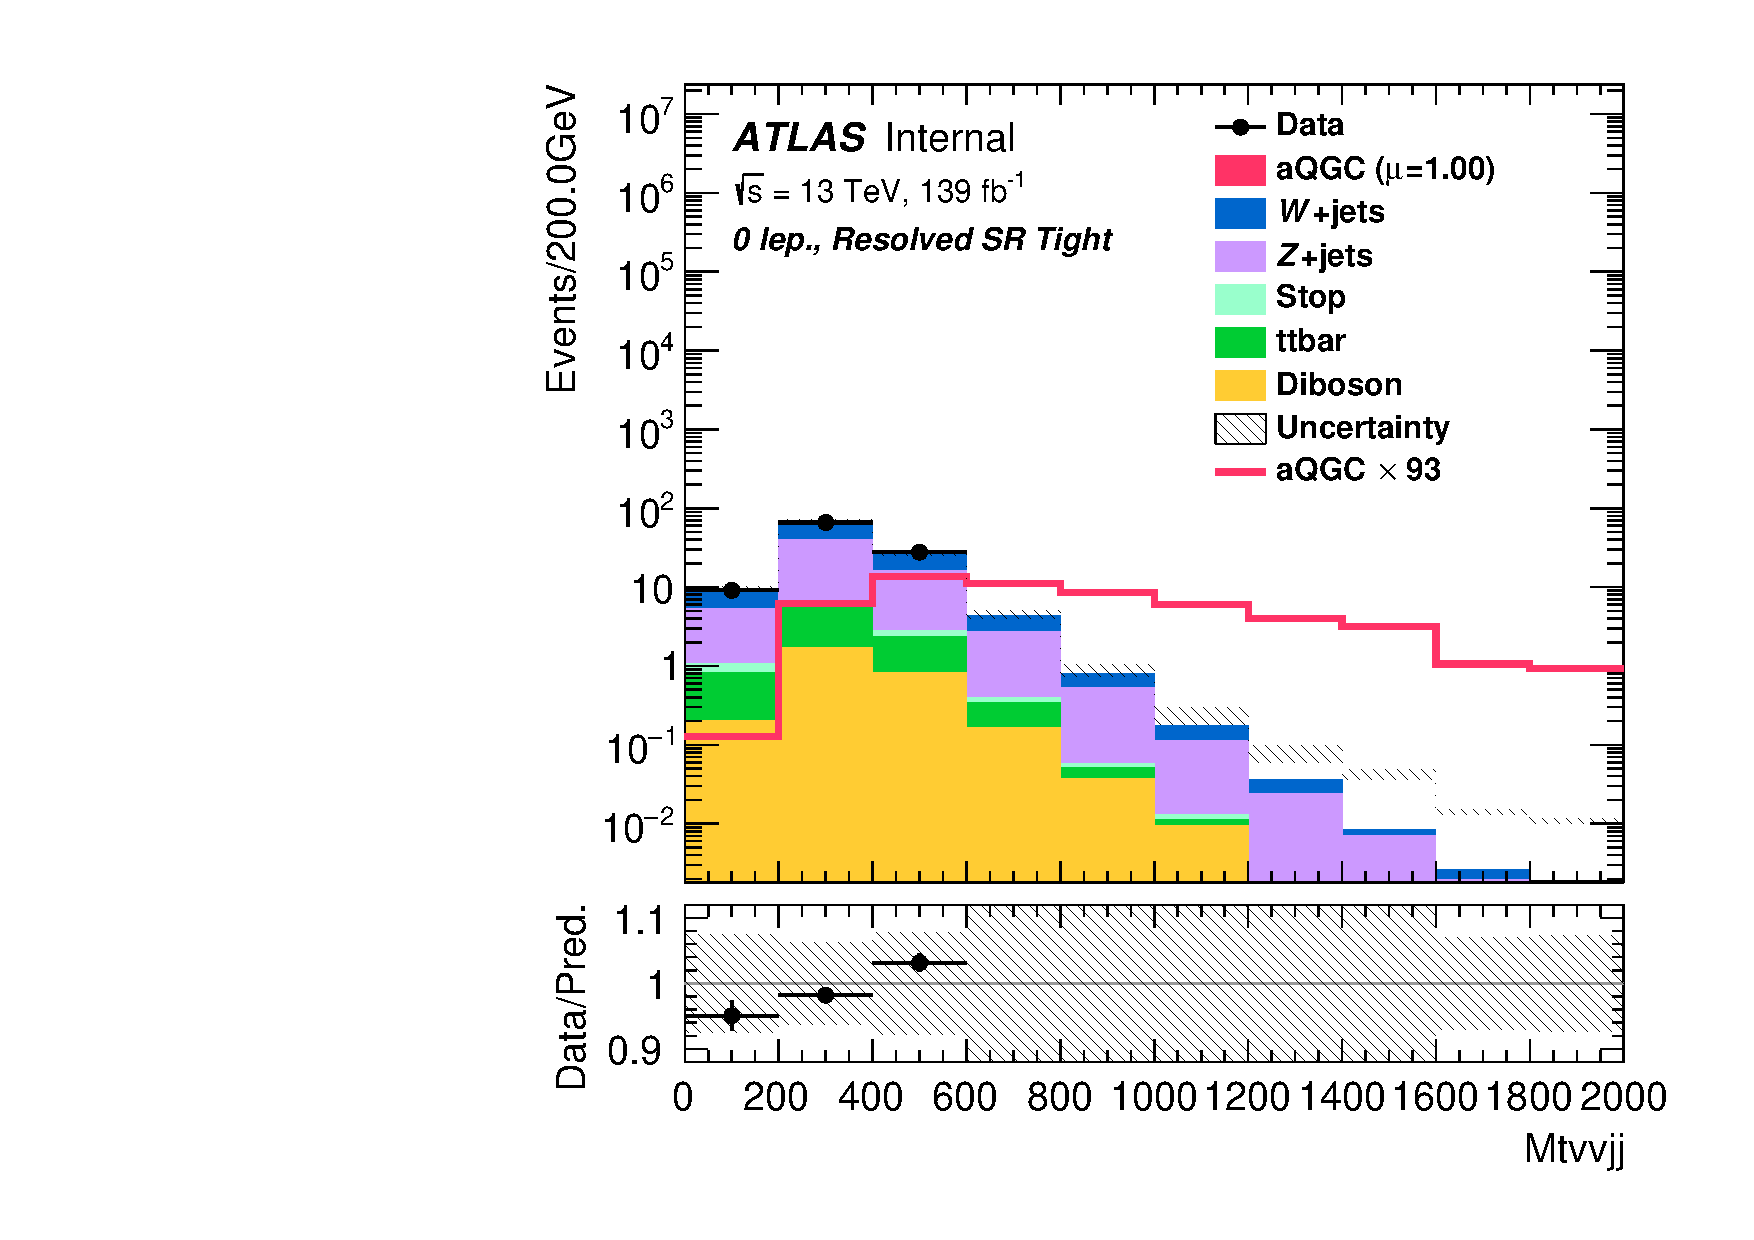
\includegraphics[width=0.32\textwidth]{figures/aQGC/MVV/Region_distMtvvjj_DSRVBSFid_BMin0_T0_Y6051_incTag1_J2_L0_incJet1_Prefitlog.pdf}
        \caption{fig: $m_{VV}$ distribution for \tlep\ (left) and Mtv distribution for \zlep\ (right)}
        \label{fig:mVVdist}
\end{figure}

\begin{table}[ht!]
\small
\begin{center}
%\resizebox{0.9\textwidth}{!}{
\begin{tabular}{ | l || l | l | l |}
\hline
Threshold values (GeV)          & SRVBS\_HP  & SRVBS\_LP & SRVBS\_Fid  \tabularnewline \hline
0-lepton & 1050      & 1200     & 1200       \tabularnewline \hline
1-lepton & 1500      & 1500     & 1500       \tabularnewline \hline
2-lepton & 1500      & 1500     & 1500       \tabularnewline \hline
\end{tabular}
\caption{Threshold values}
\label{tab:2binthreshold}
\end{center}
\end{table}

\section{Limits setting}
Finally, by using both quadratic and interference terms as a combined signal template, the expected 95\% CL upper and lower limits are obtained by the fit to the asimov dataset constructed from the background plus SM EW VV+jj samples, as well as observed limits with data.
The POI is set to include both QUAD terms and INT terms simultaneously, thereby two signal strength is parameterized as $\mu_{QUAD} = \mu_{INT}^2$.
All SRs in \zlep, \olep\, and \tlep\ channels are separated into low- and high-$m_{VV}$ bins as discussed in Section~\ref{subsec:2binapproach} and combined statistically.
All systematic uncertainties discussed for Standard Model measurement are included in the fitting.
The SM EW VV+jj signal samples are added to the background as a free floated normalization factor, and all the analysis regions are correlated with EW VV+jj signal samplee.
Due to the small statistics in high-$m_{VV}$ regions compared with the low-$m_{VV}$ regions, the overall behaviors of the post-fit nuisance parameters are almost the same as the SM measurement.
The expected on observed limits are shown at 5 clipping energy points of [1.5, 2.0, 3.0, 5.0, $\infty$]~TeV in Figure~\ref{fig:aQGClimits}.
The unitarity bound from the theoretical calculation \cite{PhysRevD.101.113003} is overlaid.
%The upper and lower limits correspond to the signal hypotheses showing $\Delta NLL \sim \frac{1}{2}\chi^2 = 1.0$.

The log-likelihood (-2 ln $\lambda$; $\lambda$ is a likelihood ratio) distributions with respect to the signal strength of aQGC signal, $\mu_{\mathrm{aQGC}}$, is shown in figure~\ref{fig:ProfileLL},\ref{fig:ProfileLLFS}, \ref{fig:ProfileLLFM} for FT0, FS02, FM0 operator, for each clipping energy of 1500~GeV, 2000~GeV, $\infty$.
%Figure~\ref{}, \ref{}, \ref{} show the log-likelihood curve obtained by the fitting with observed data for each clipping energy, for FT0, FS02, FM0 operators, respectively.
\begin{figure}[ht]
    \centering
    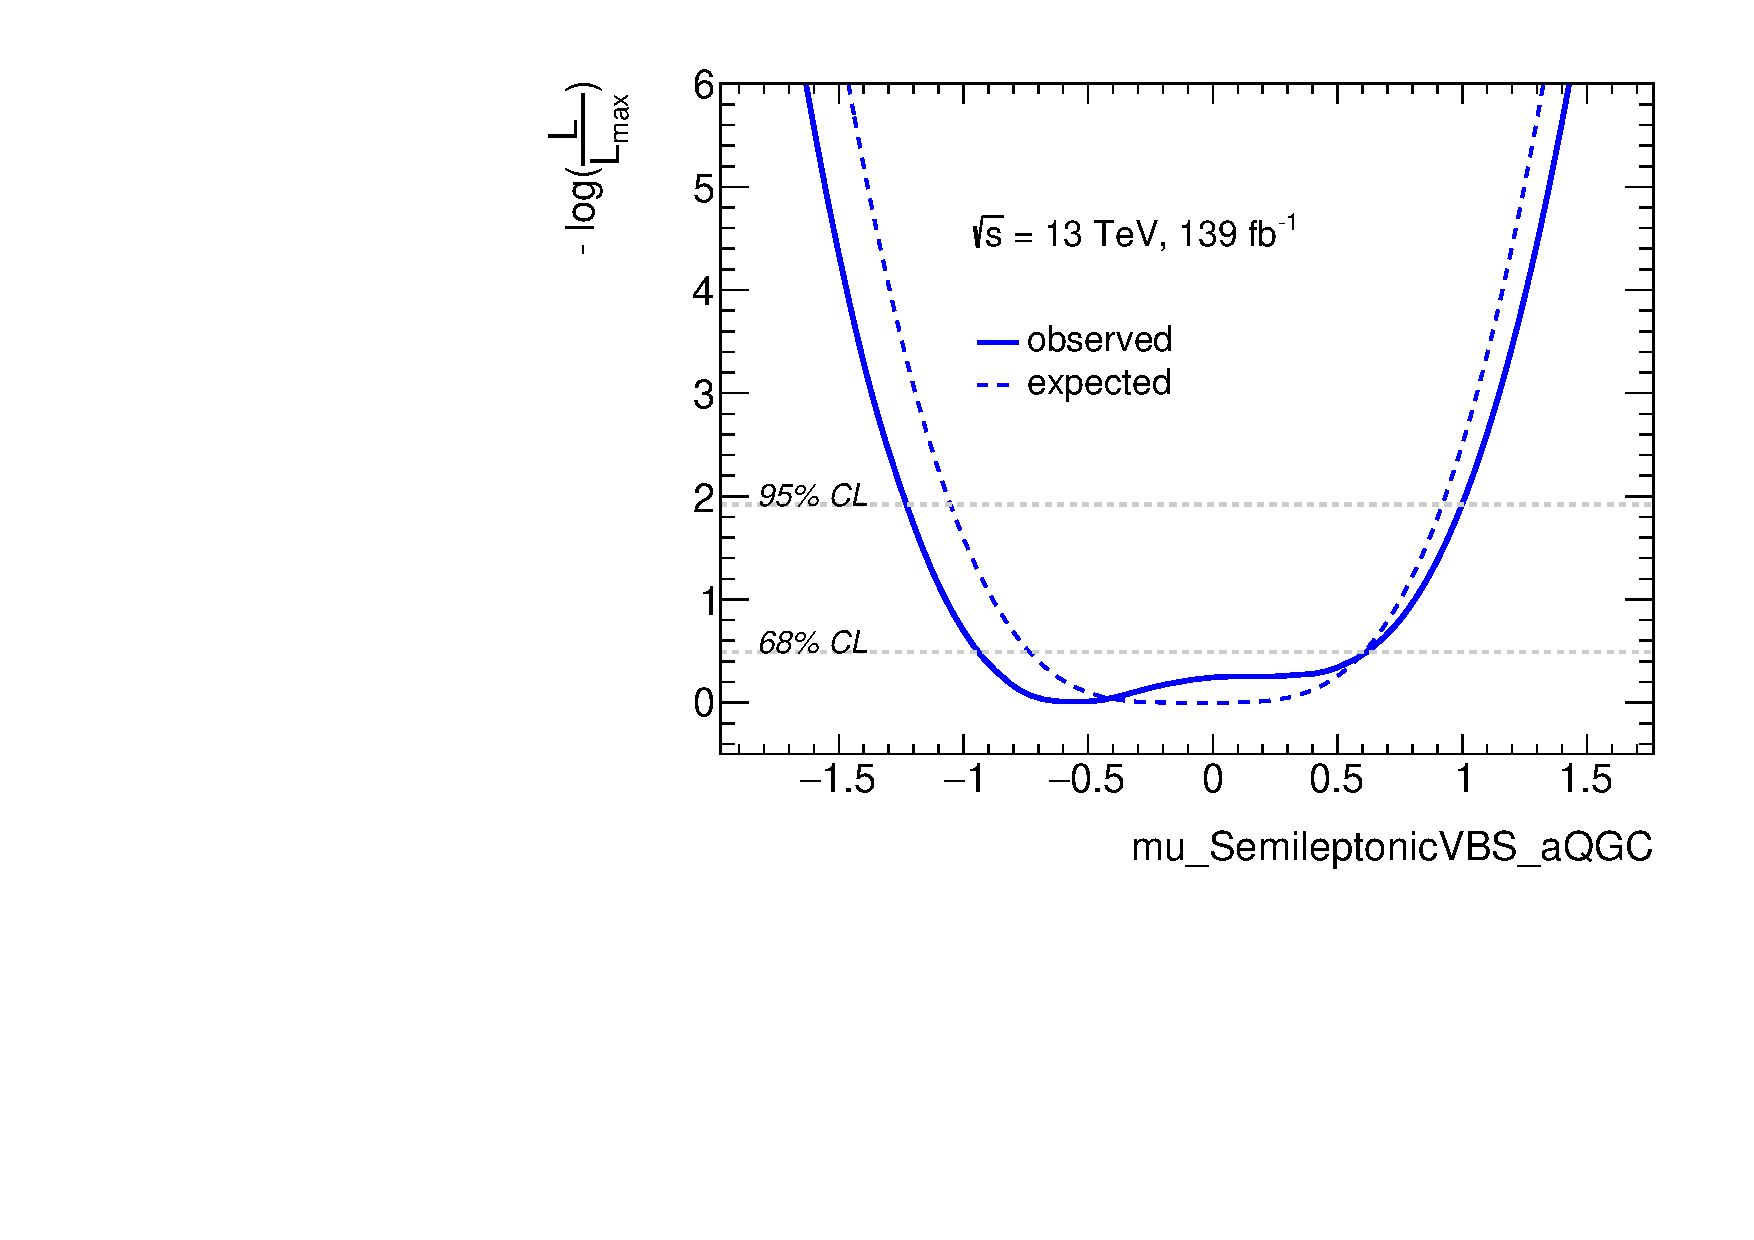
\includegraphics[width=0.32\textwidth]{figures/aQGC/profileFT01500}
    	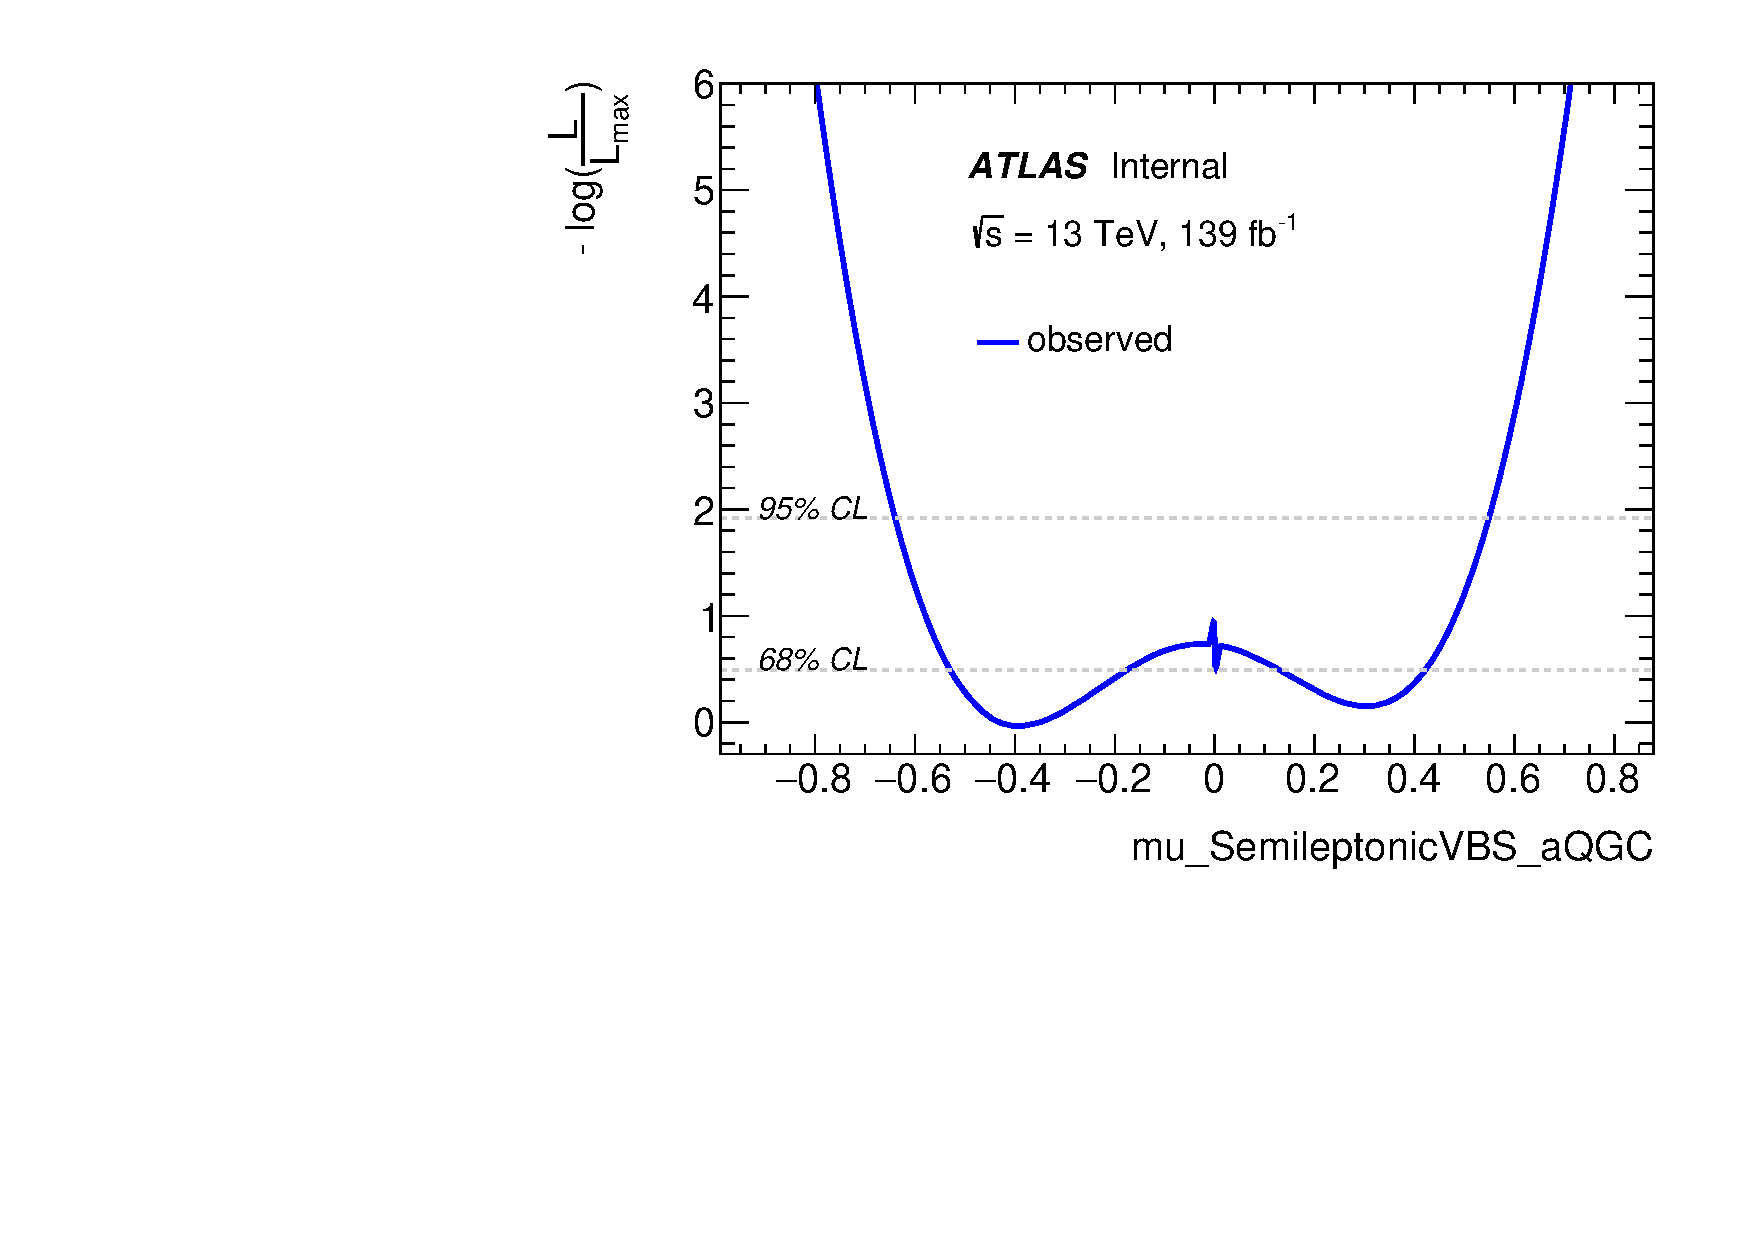
\includegraphics[width=0.32\textwidth]{figures/aQGC/profileFT02000}
    	%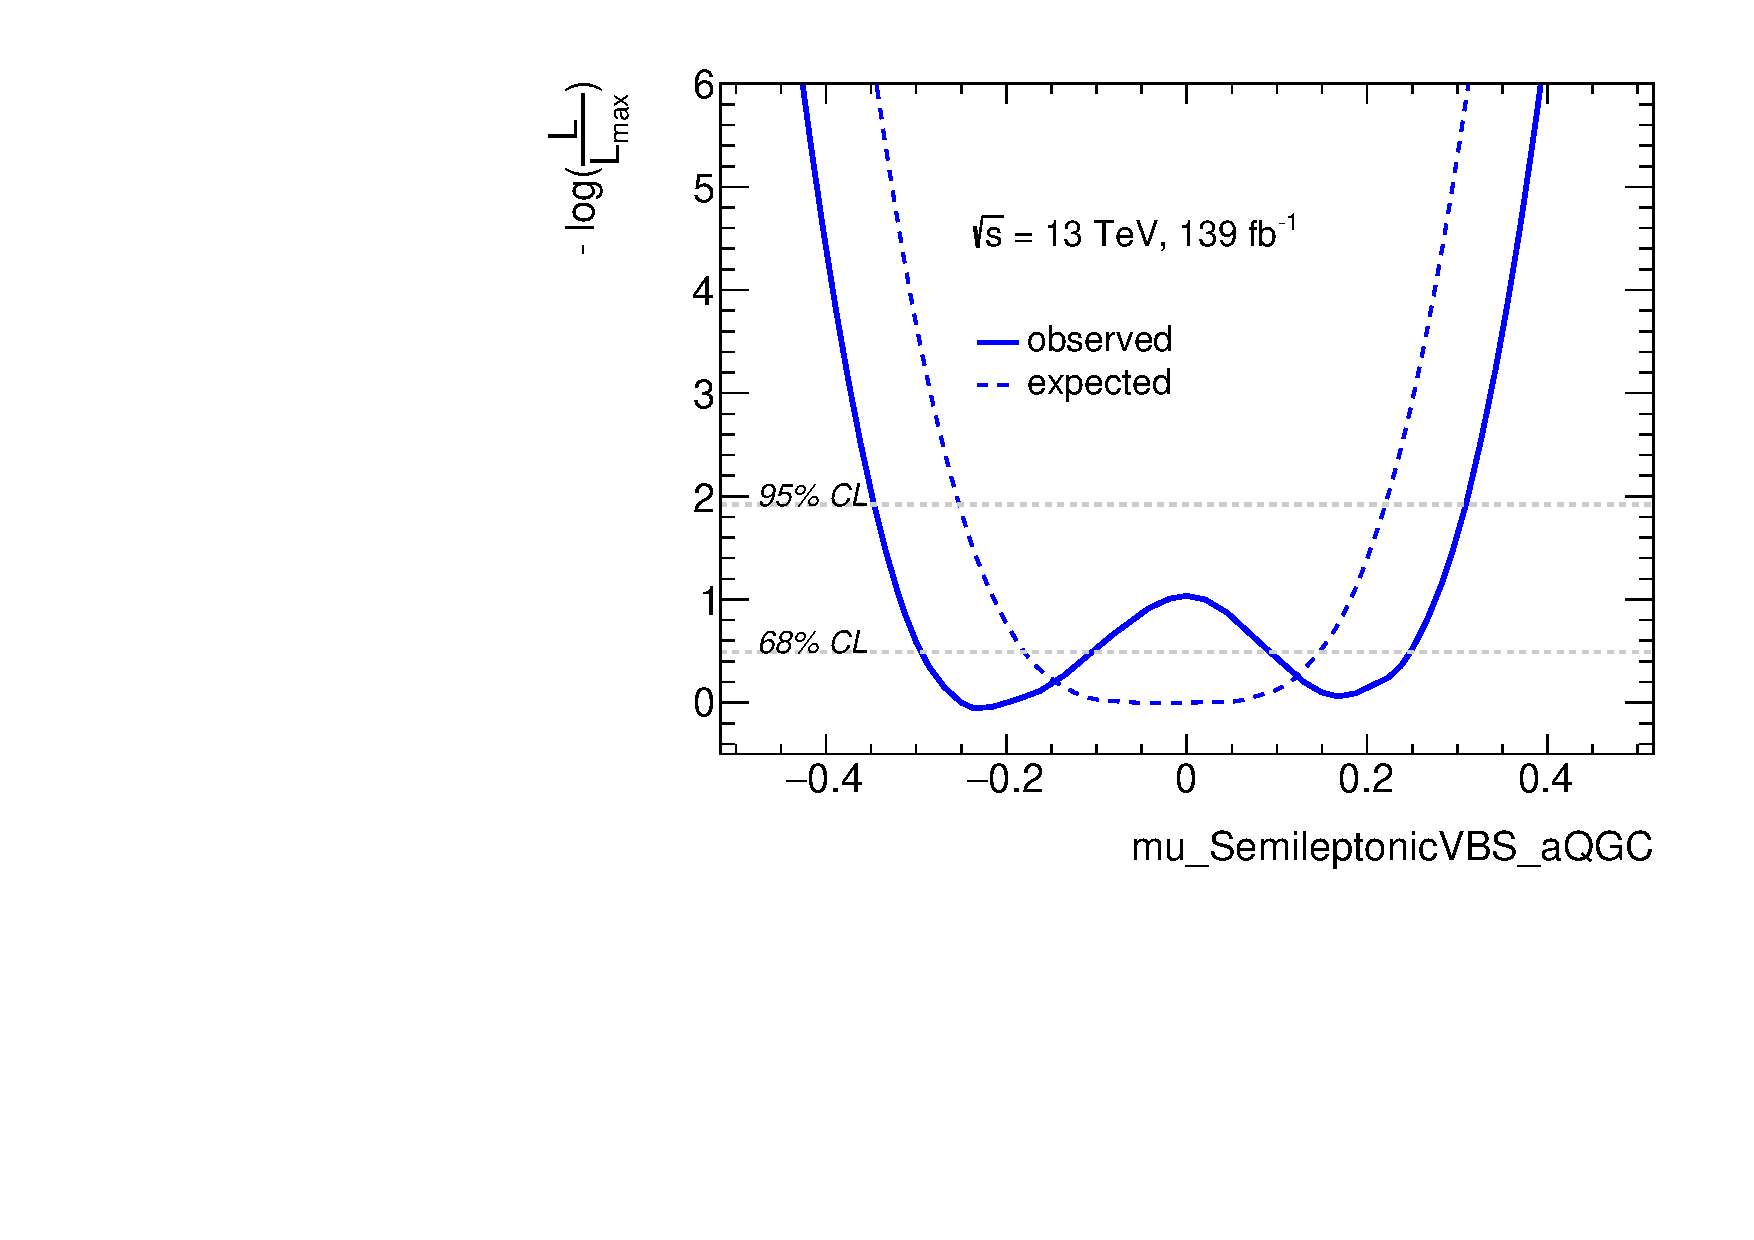
\includegraphics[width=0.38\textwidth]{figures/aQGC/profileFT03000}
        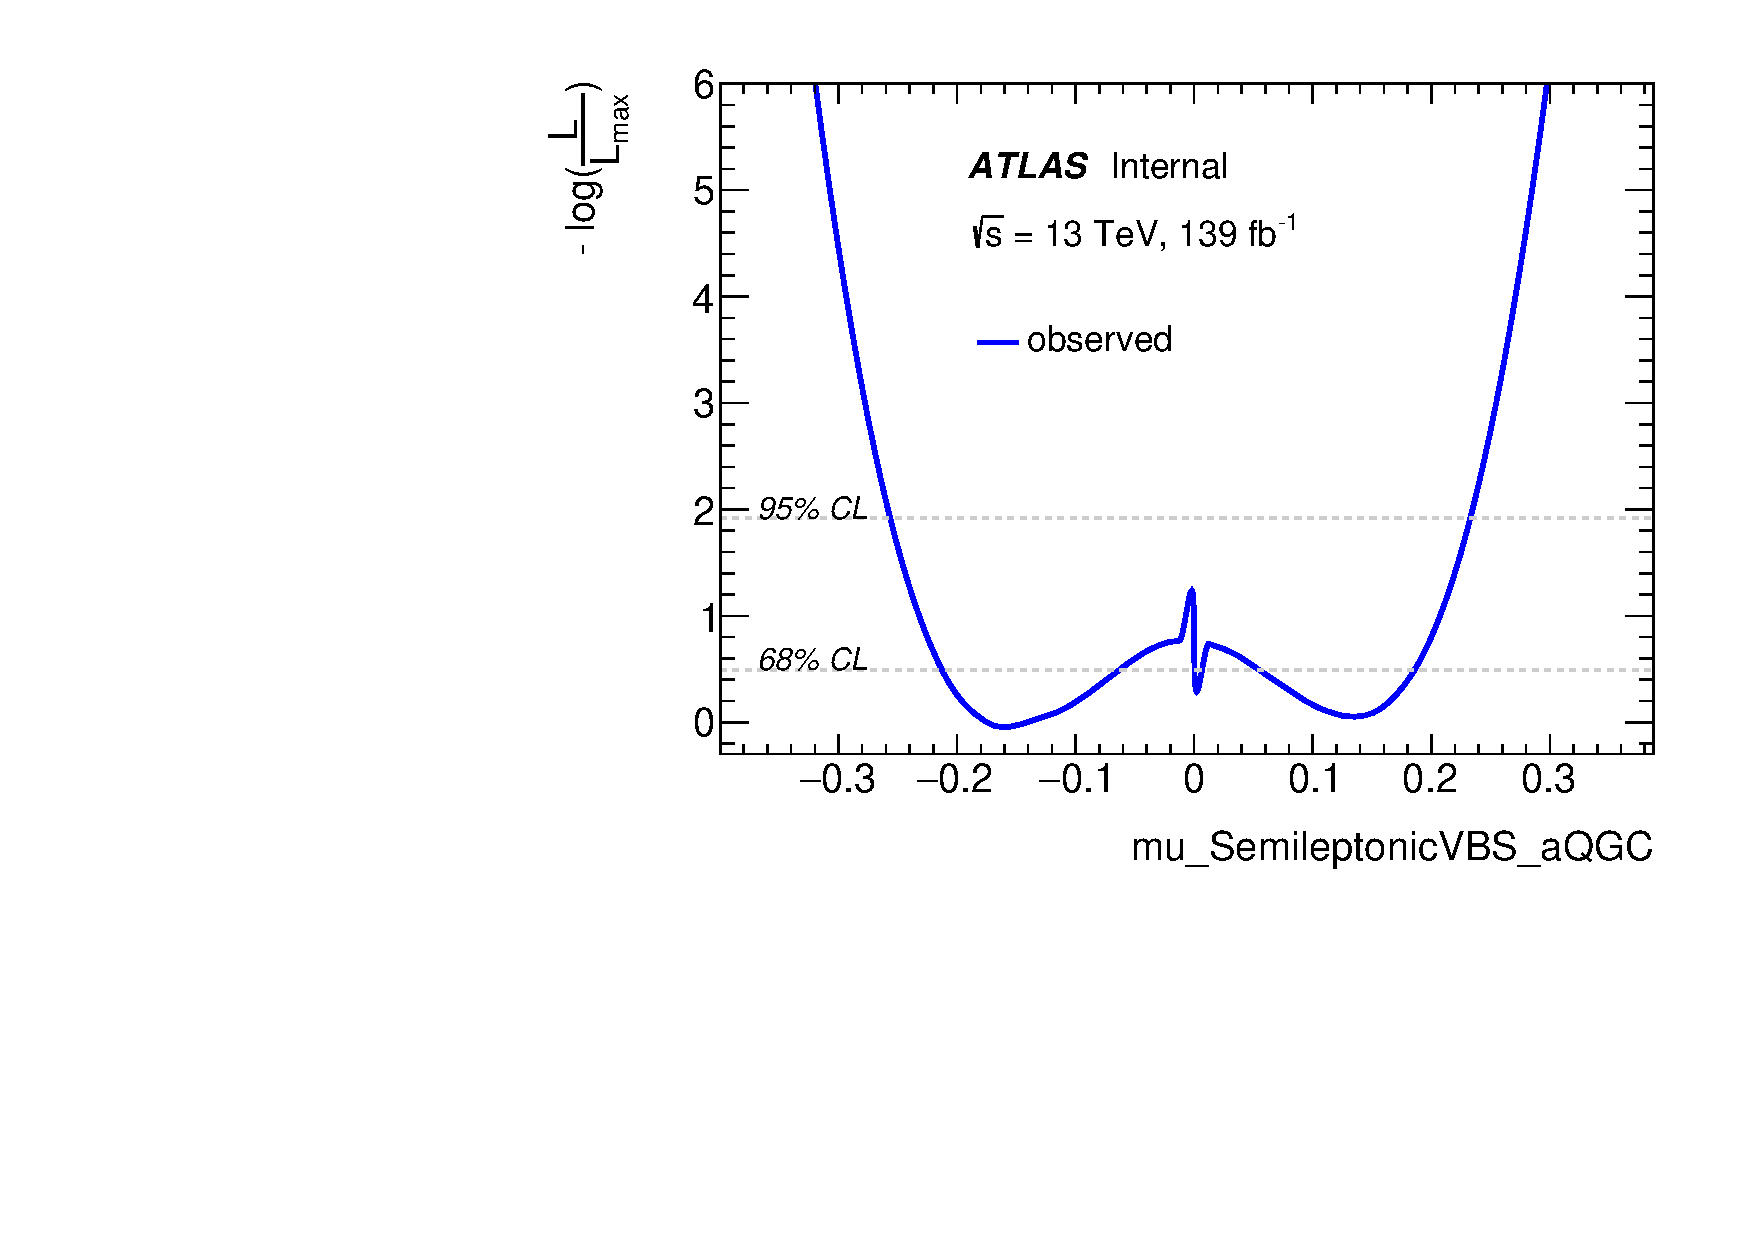
\includegraphics[width=0.32\textwidth]{figures/aQGC/profileFT0inf}
        \caption{The observed log-likelihood curves of FT0 Wilson coefficient where the clipping energy is 1.5~TeV (left), 2.0~TeV (middle), $\infty$ (right).}
        \label{fig:ProfileLL}
\end{figure}
\begin{figure}[ht]
    \centering
    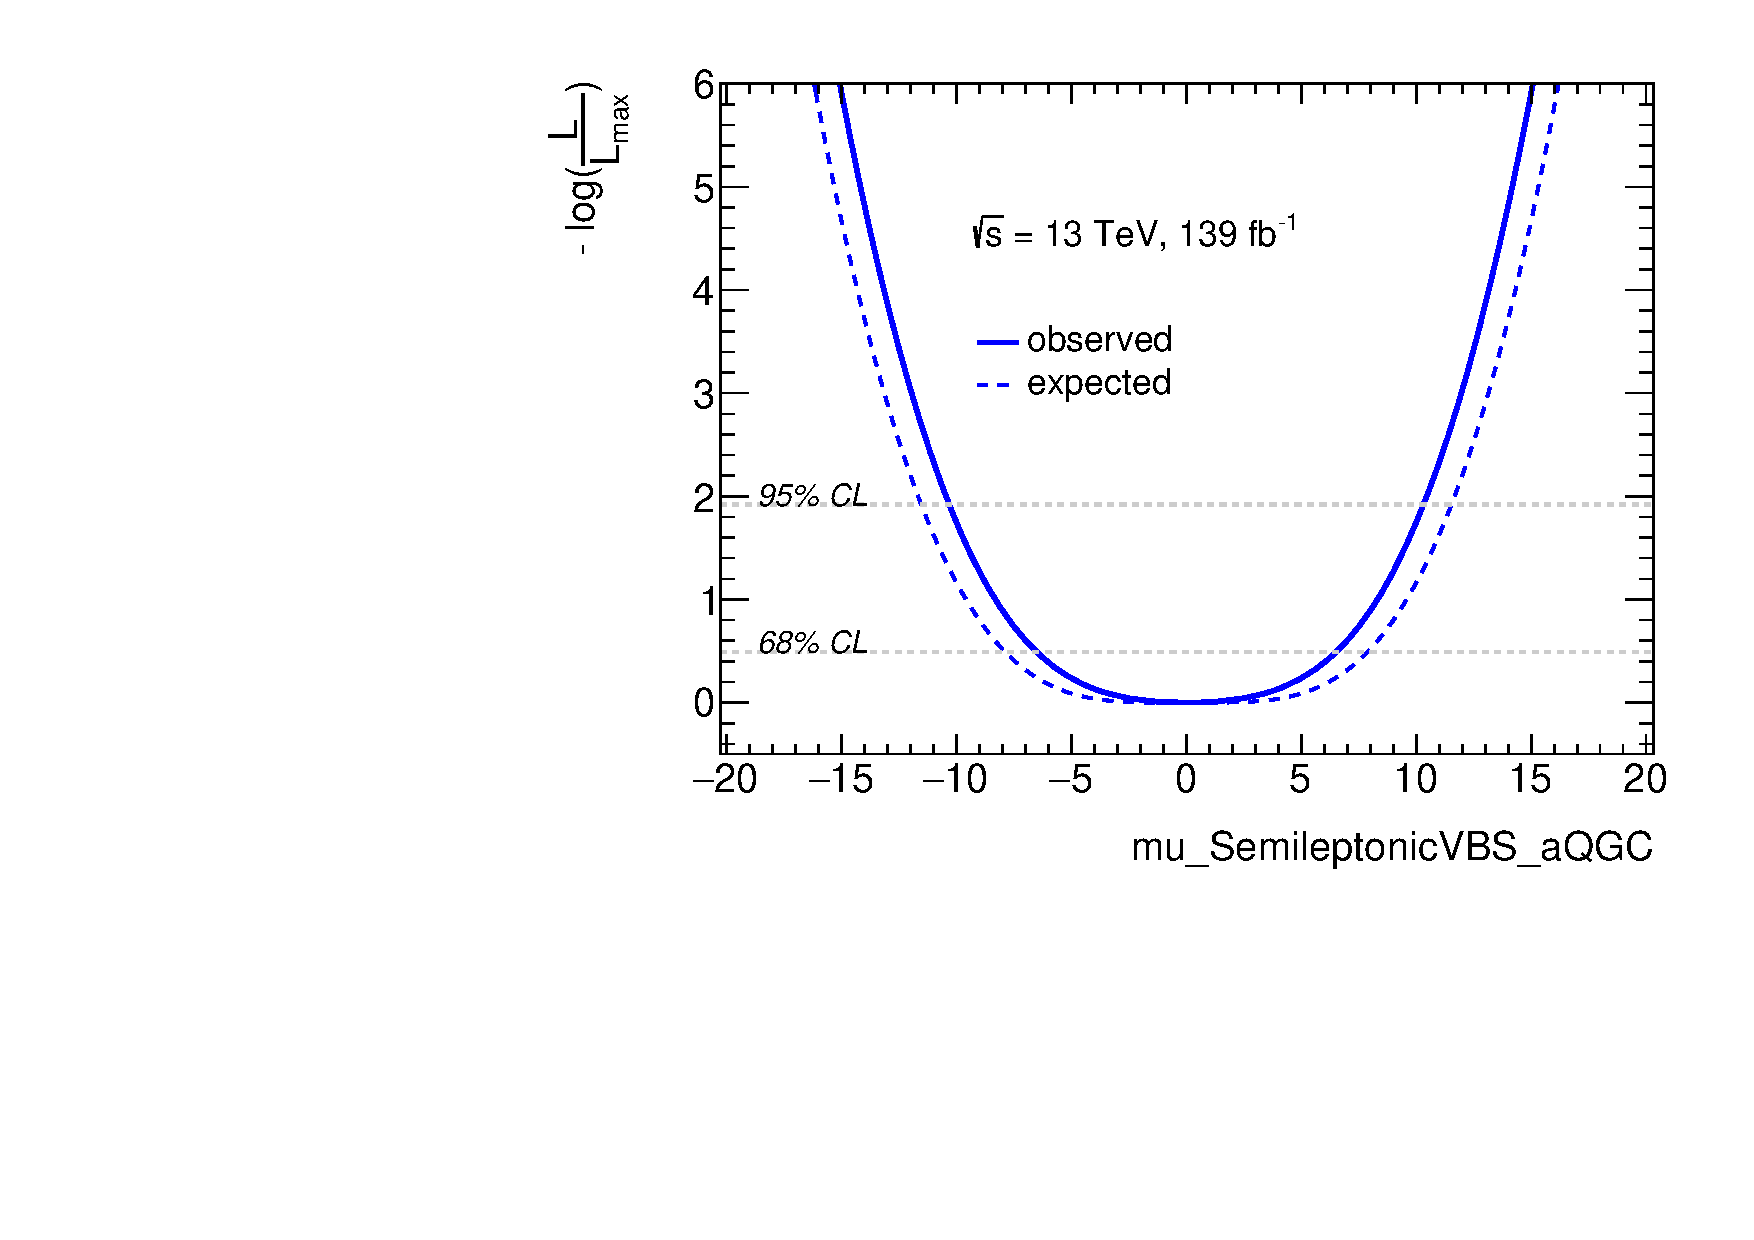
\includegraphics[width=0.32\textwidth]{figures/aQGC/profileFS021500}
    	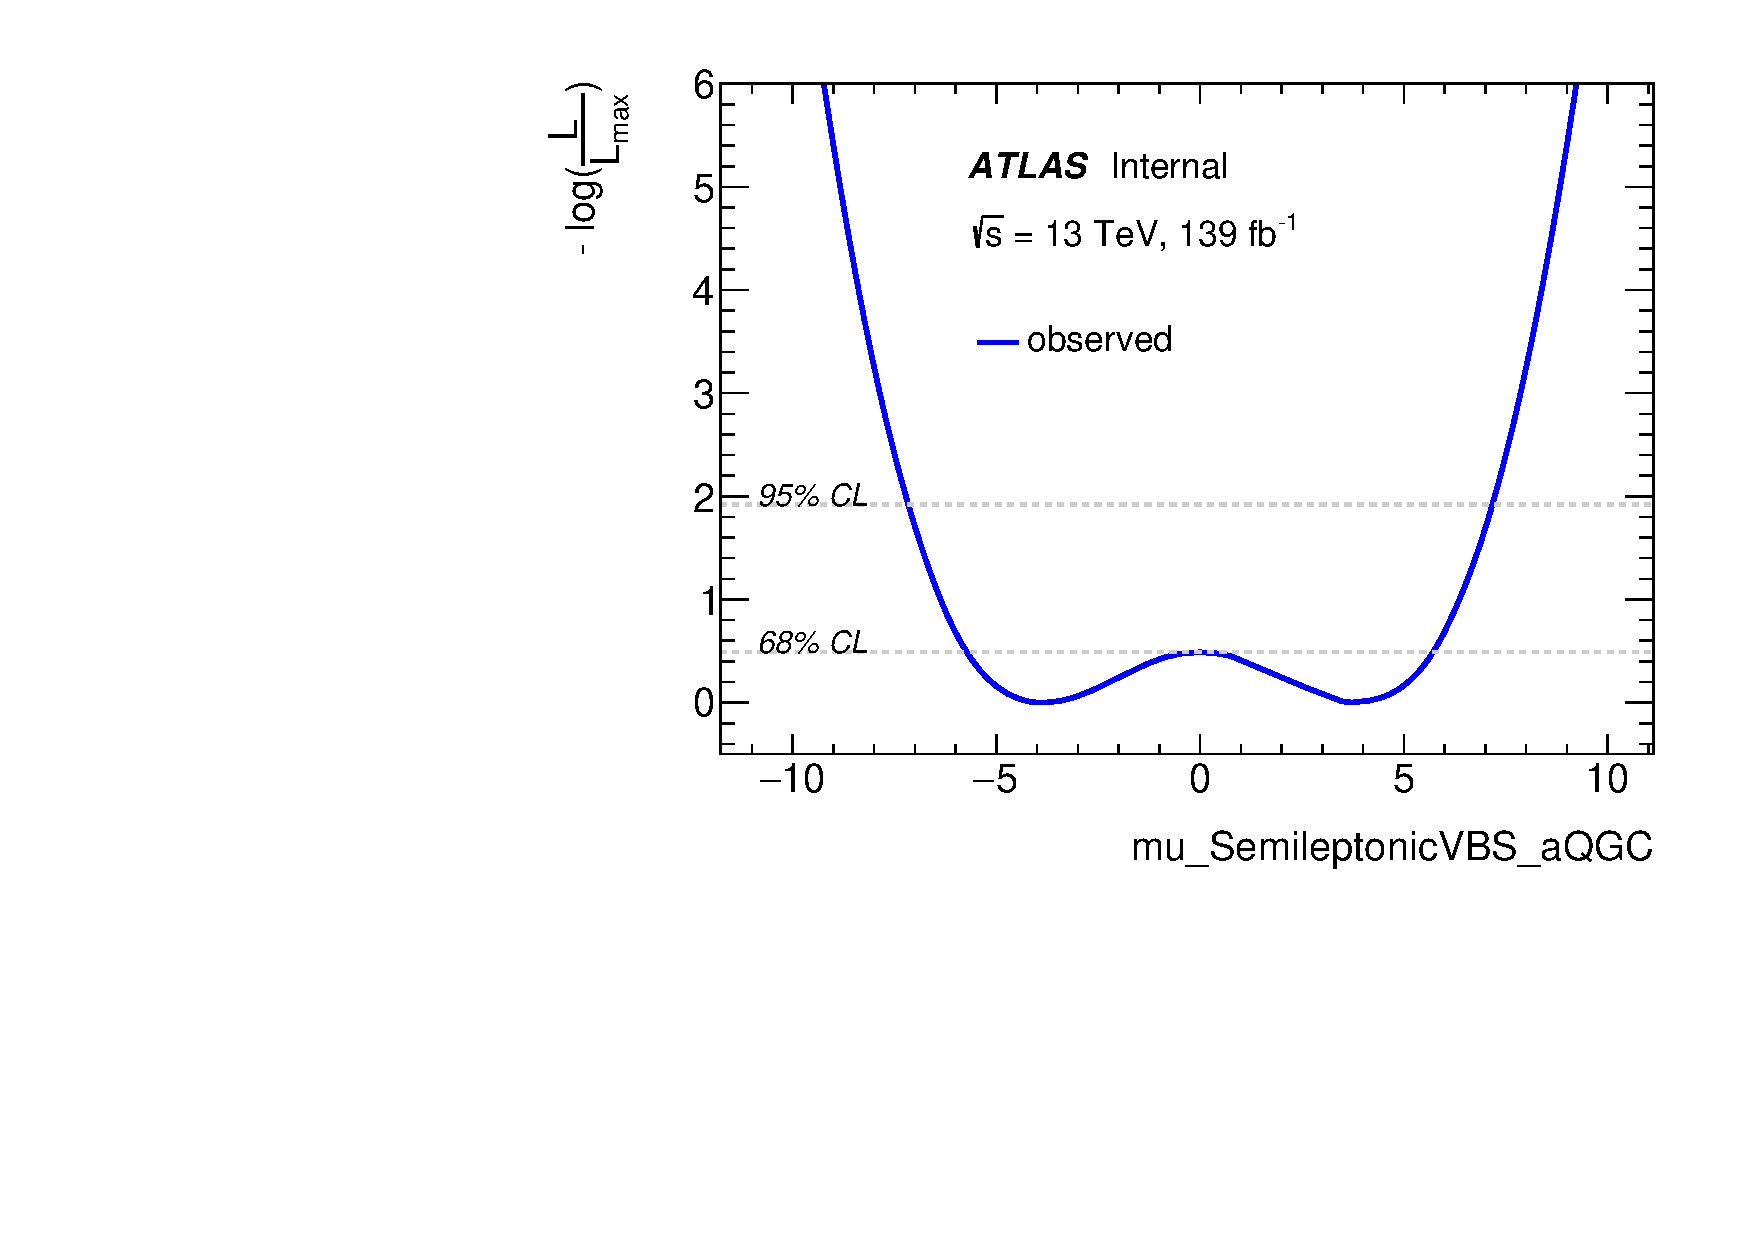
\includegraphics[width=0.32\textwidth]{figures/aQGC/profileFS022000}
    	%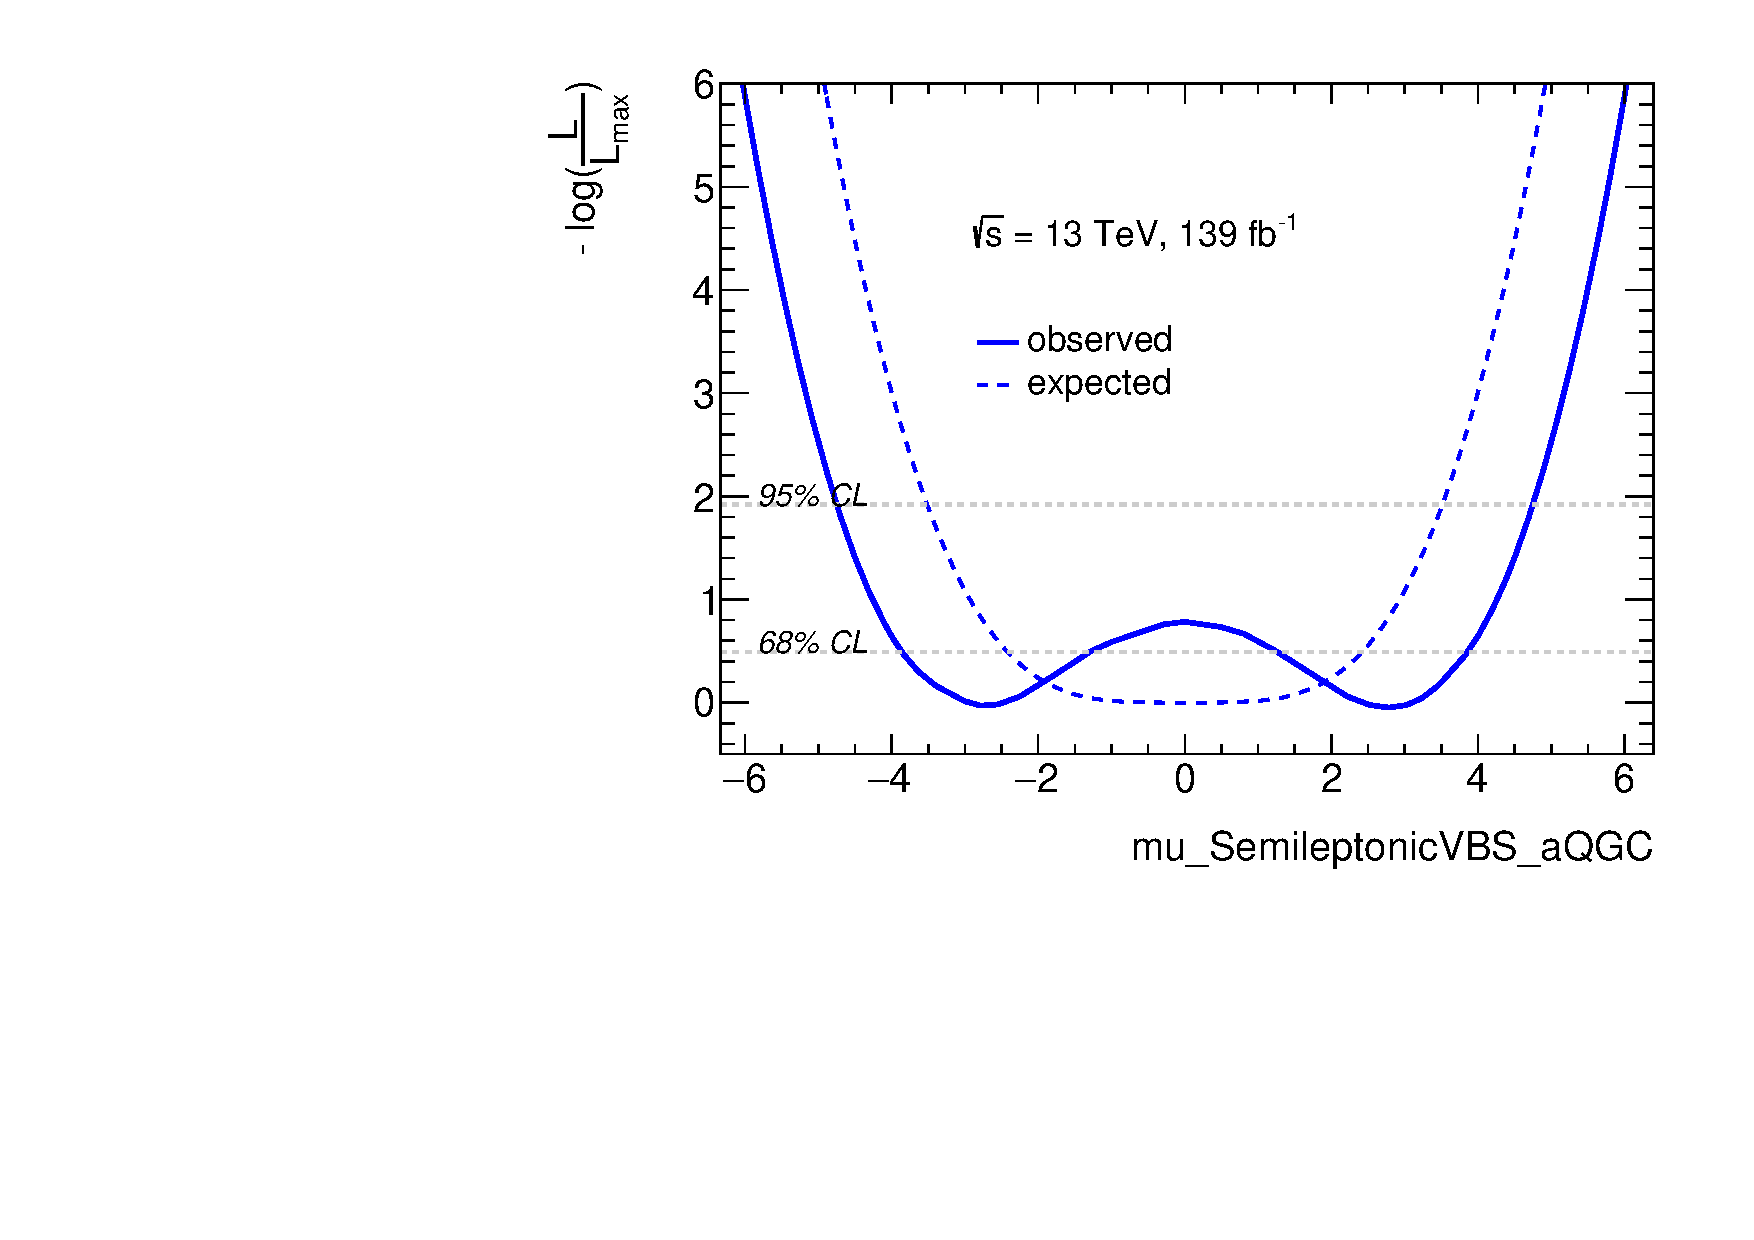
\includegraphics[width=0.38\textwidth]{figures/aQGC/profileFS023000}
        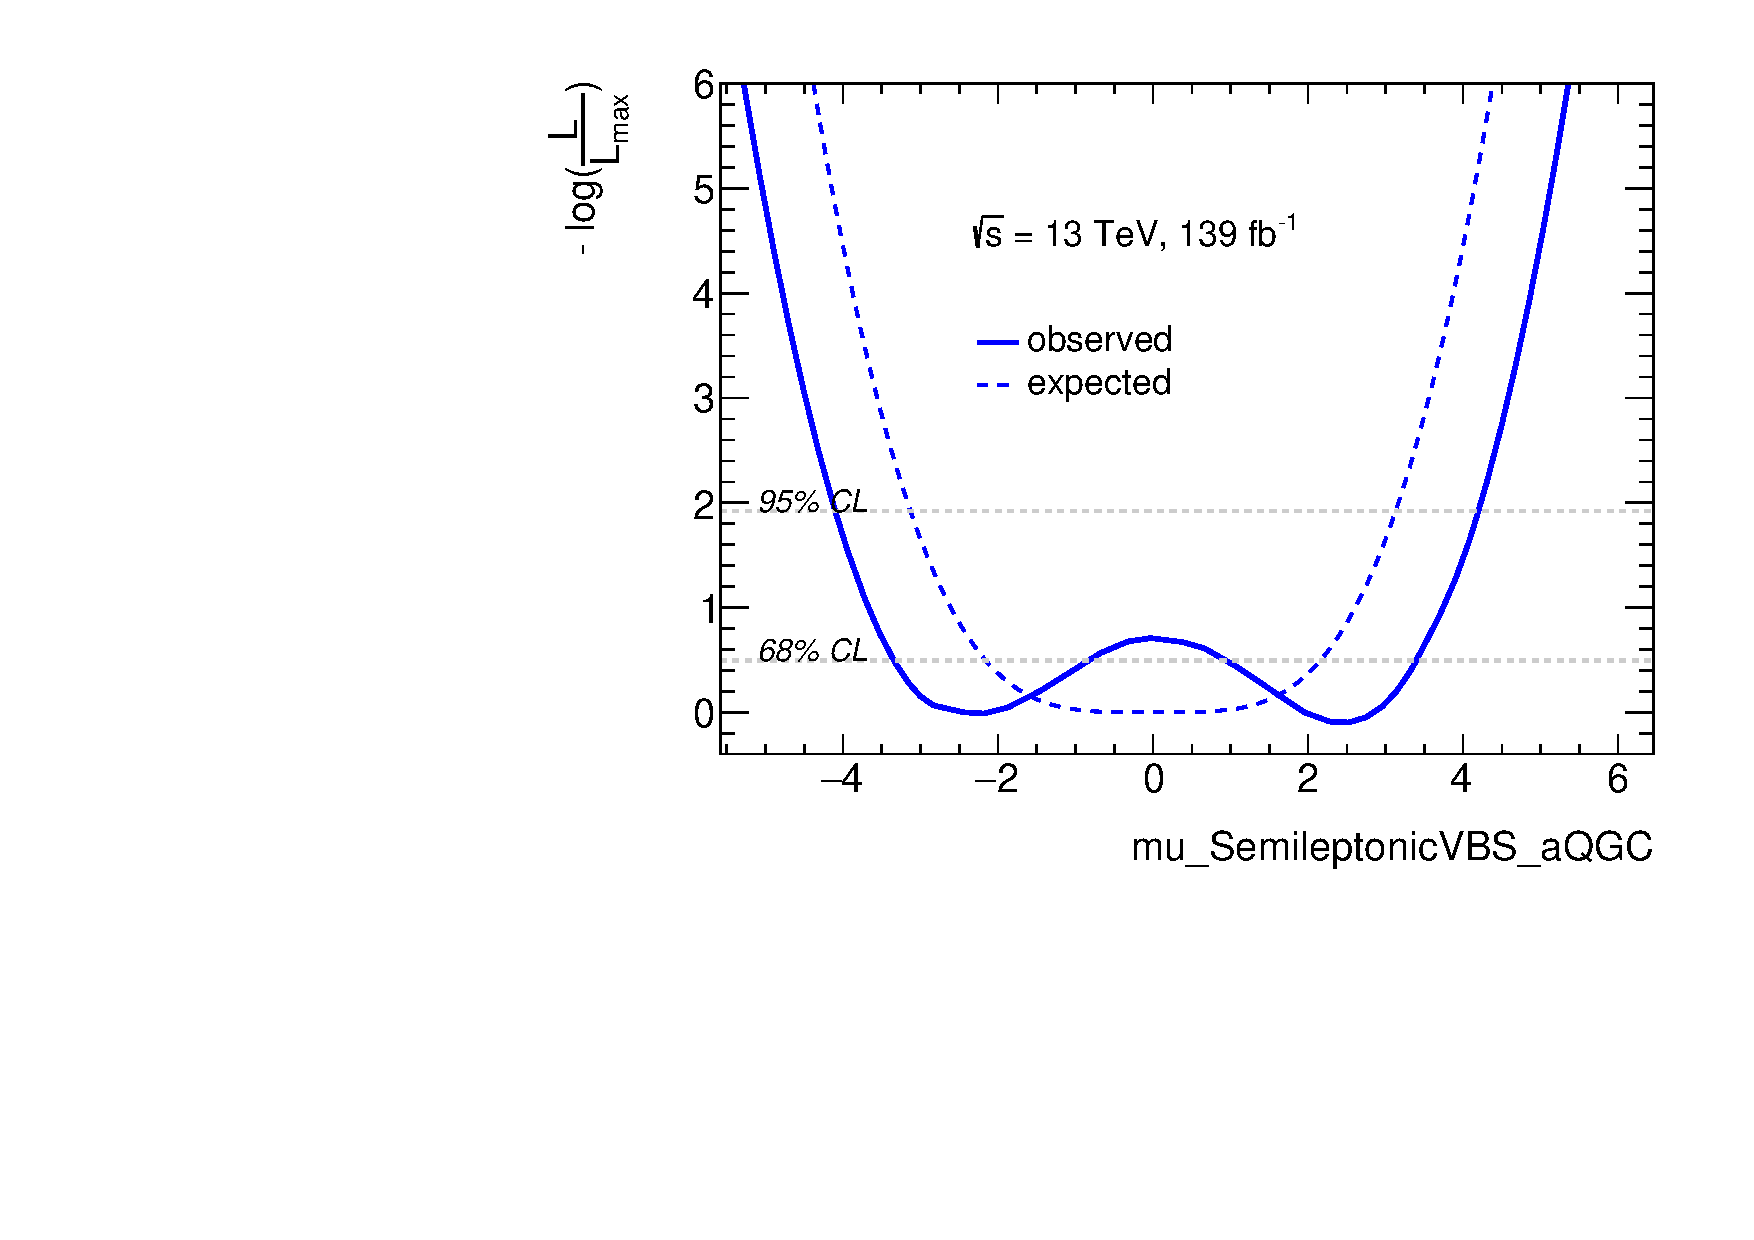
\includegraphics[width=0.32\textwidth]{figures/aQGC/profileFS02inf}
        \caption{The observed log-likelihood curves of FS02 Wilson coefficient where the clipping energy is 1.5~TeV (left), 2.0~TeV (middle), $\infty$ (right).}
        \label{fig:ProfileLLFS}
\end{figure}
\begin{figure}[ht]
    \centering
    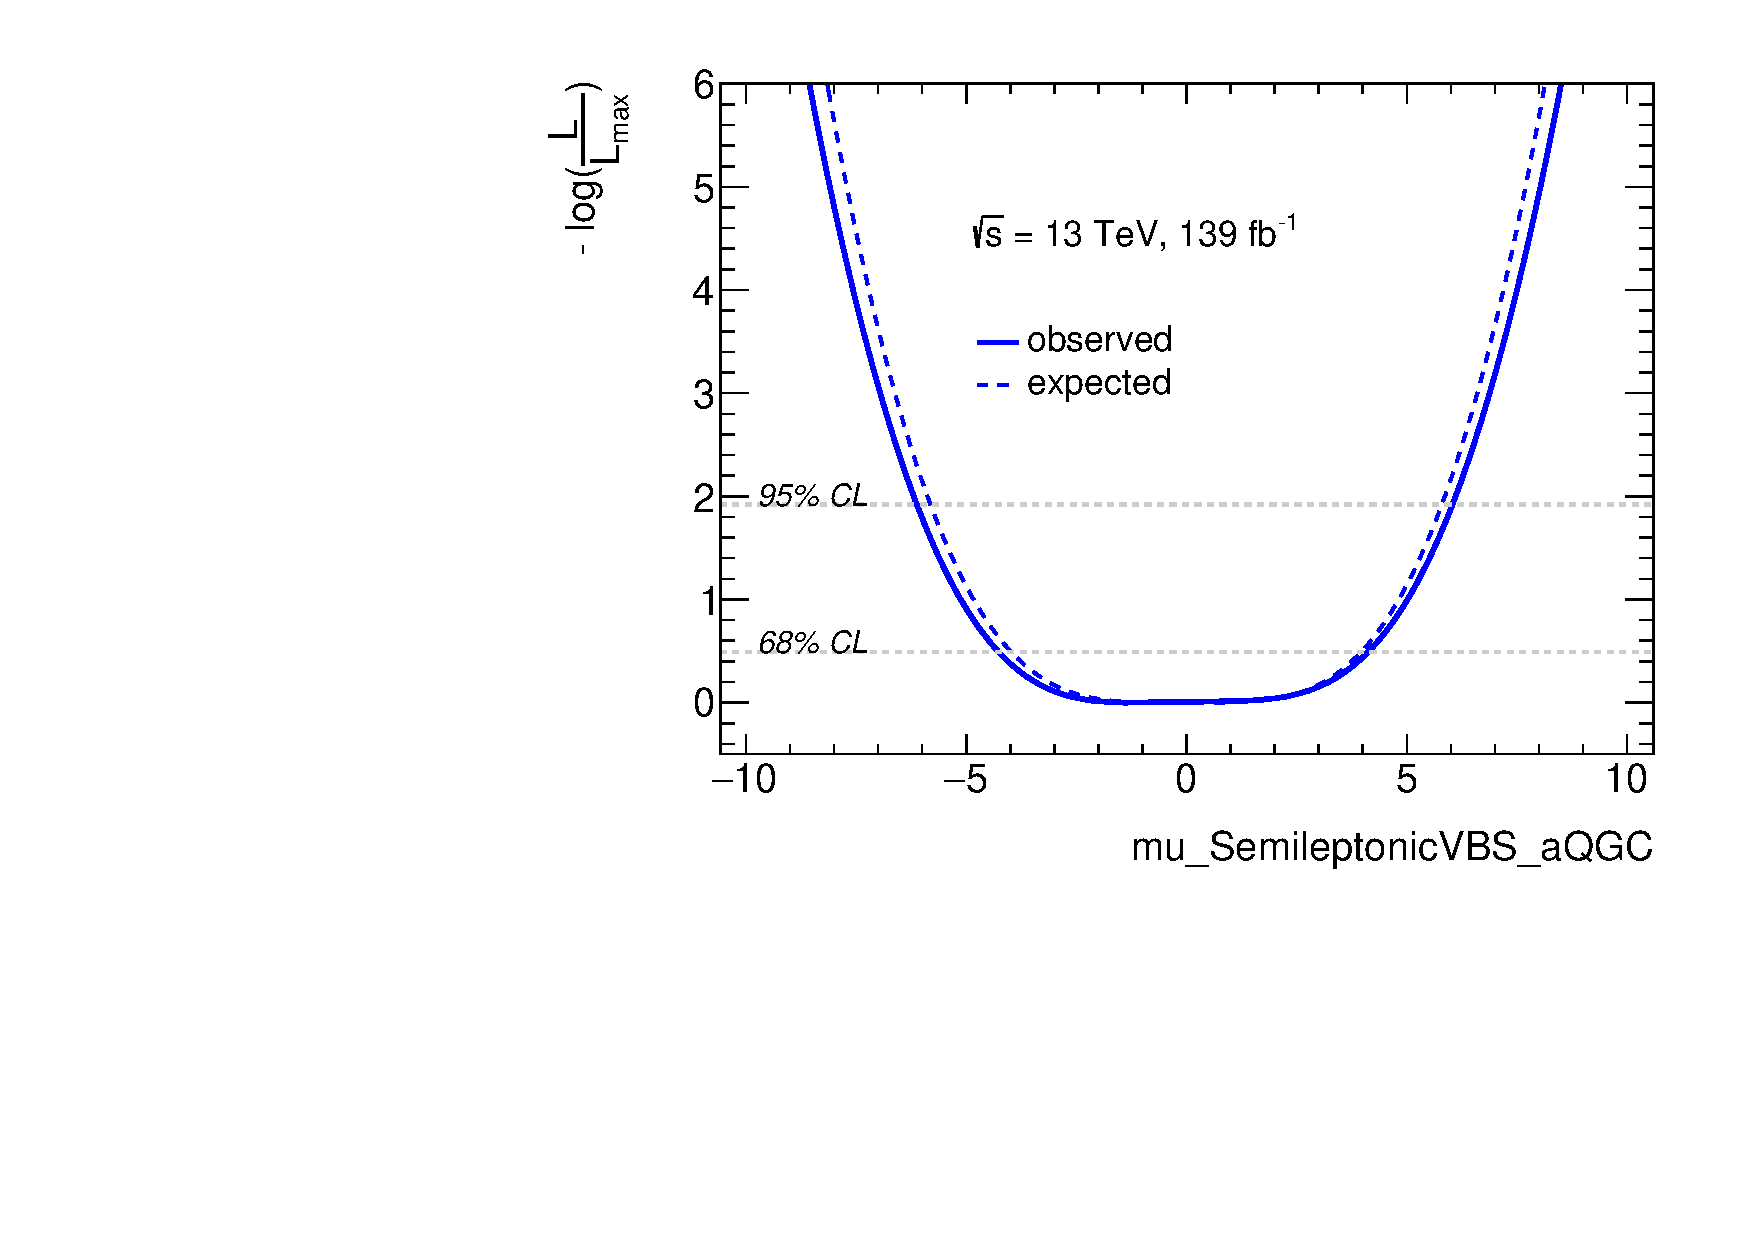
\includegraphics[width=0.32\textwidth]{figures/aQGC/profileFM01500}
    	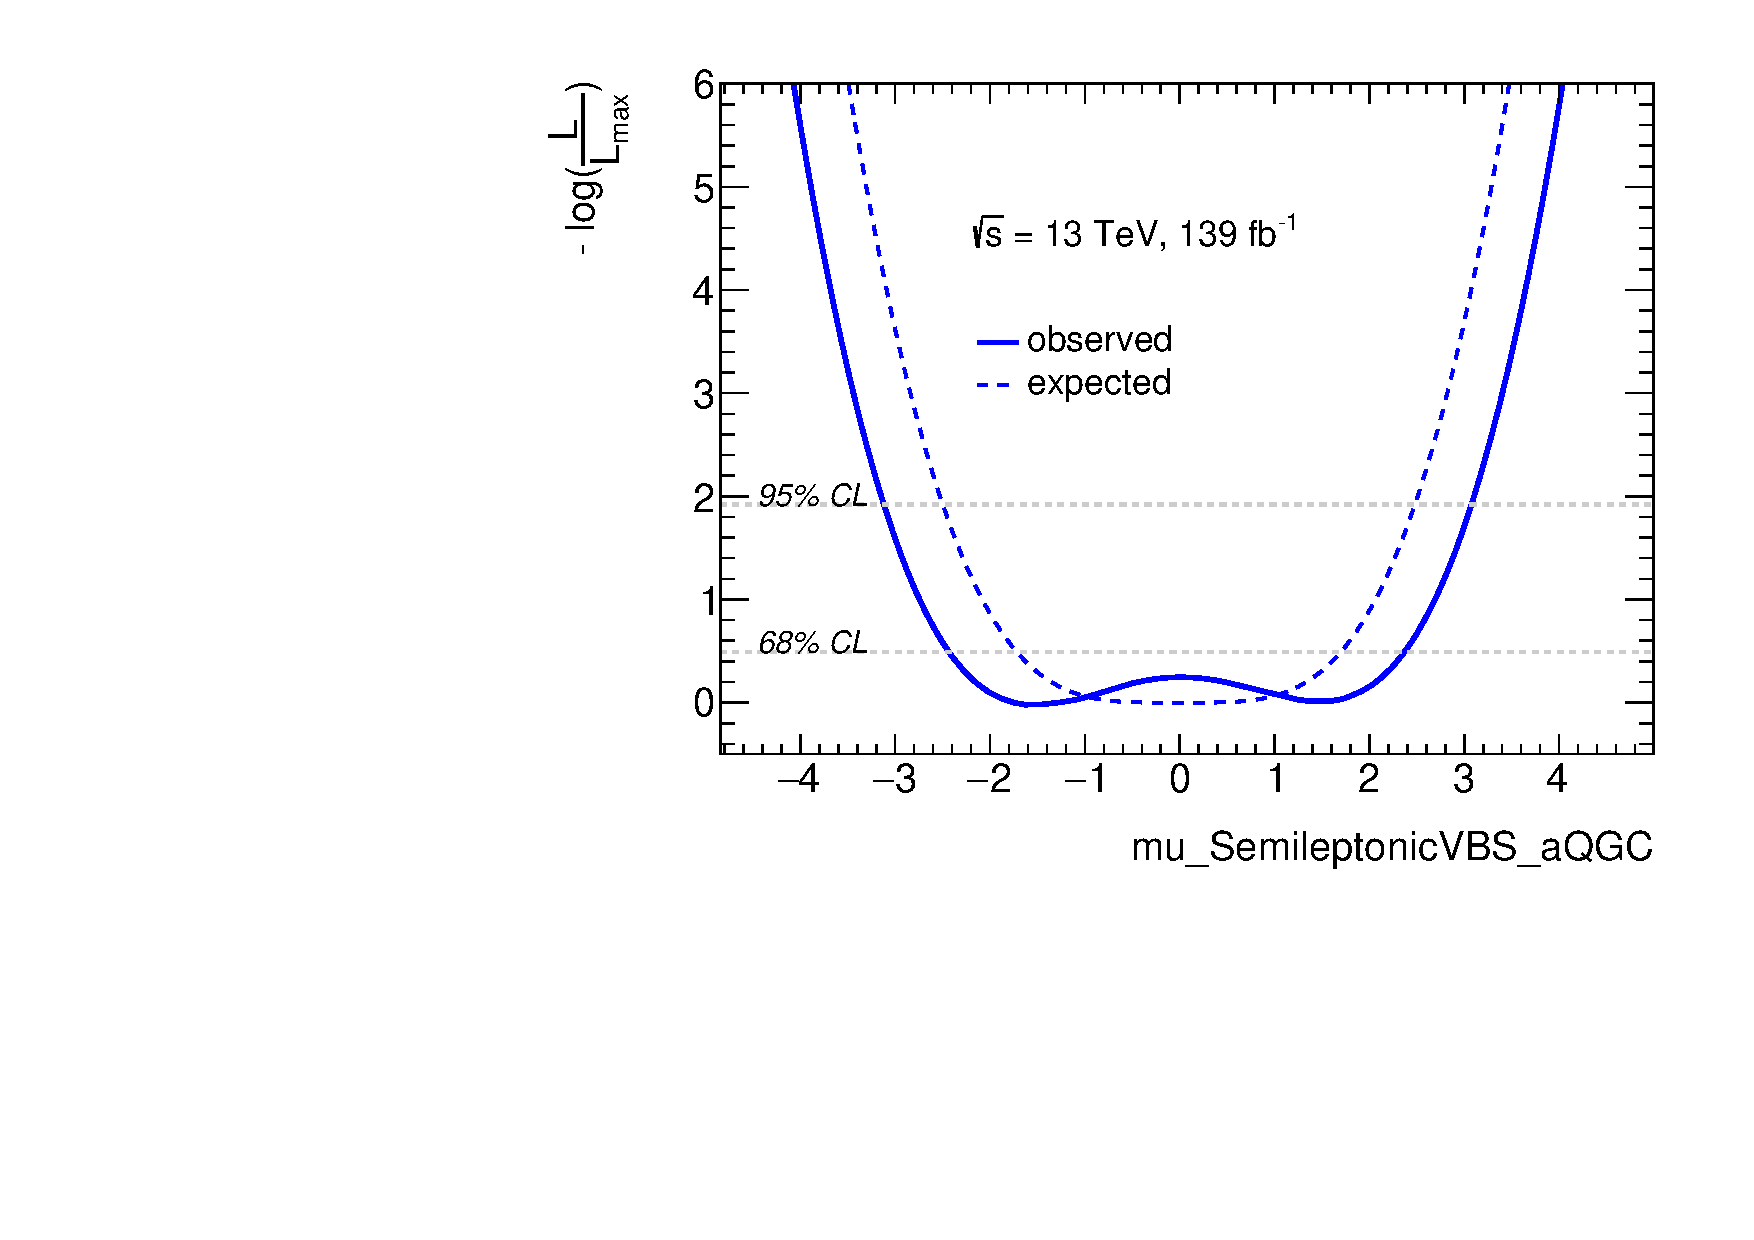
\includegraphics[width=0.32\textwidth]{figures/aQGC/profileFM02000}
    	%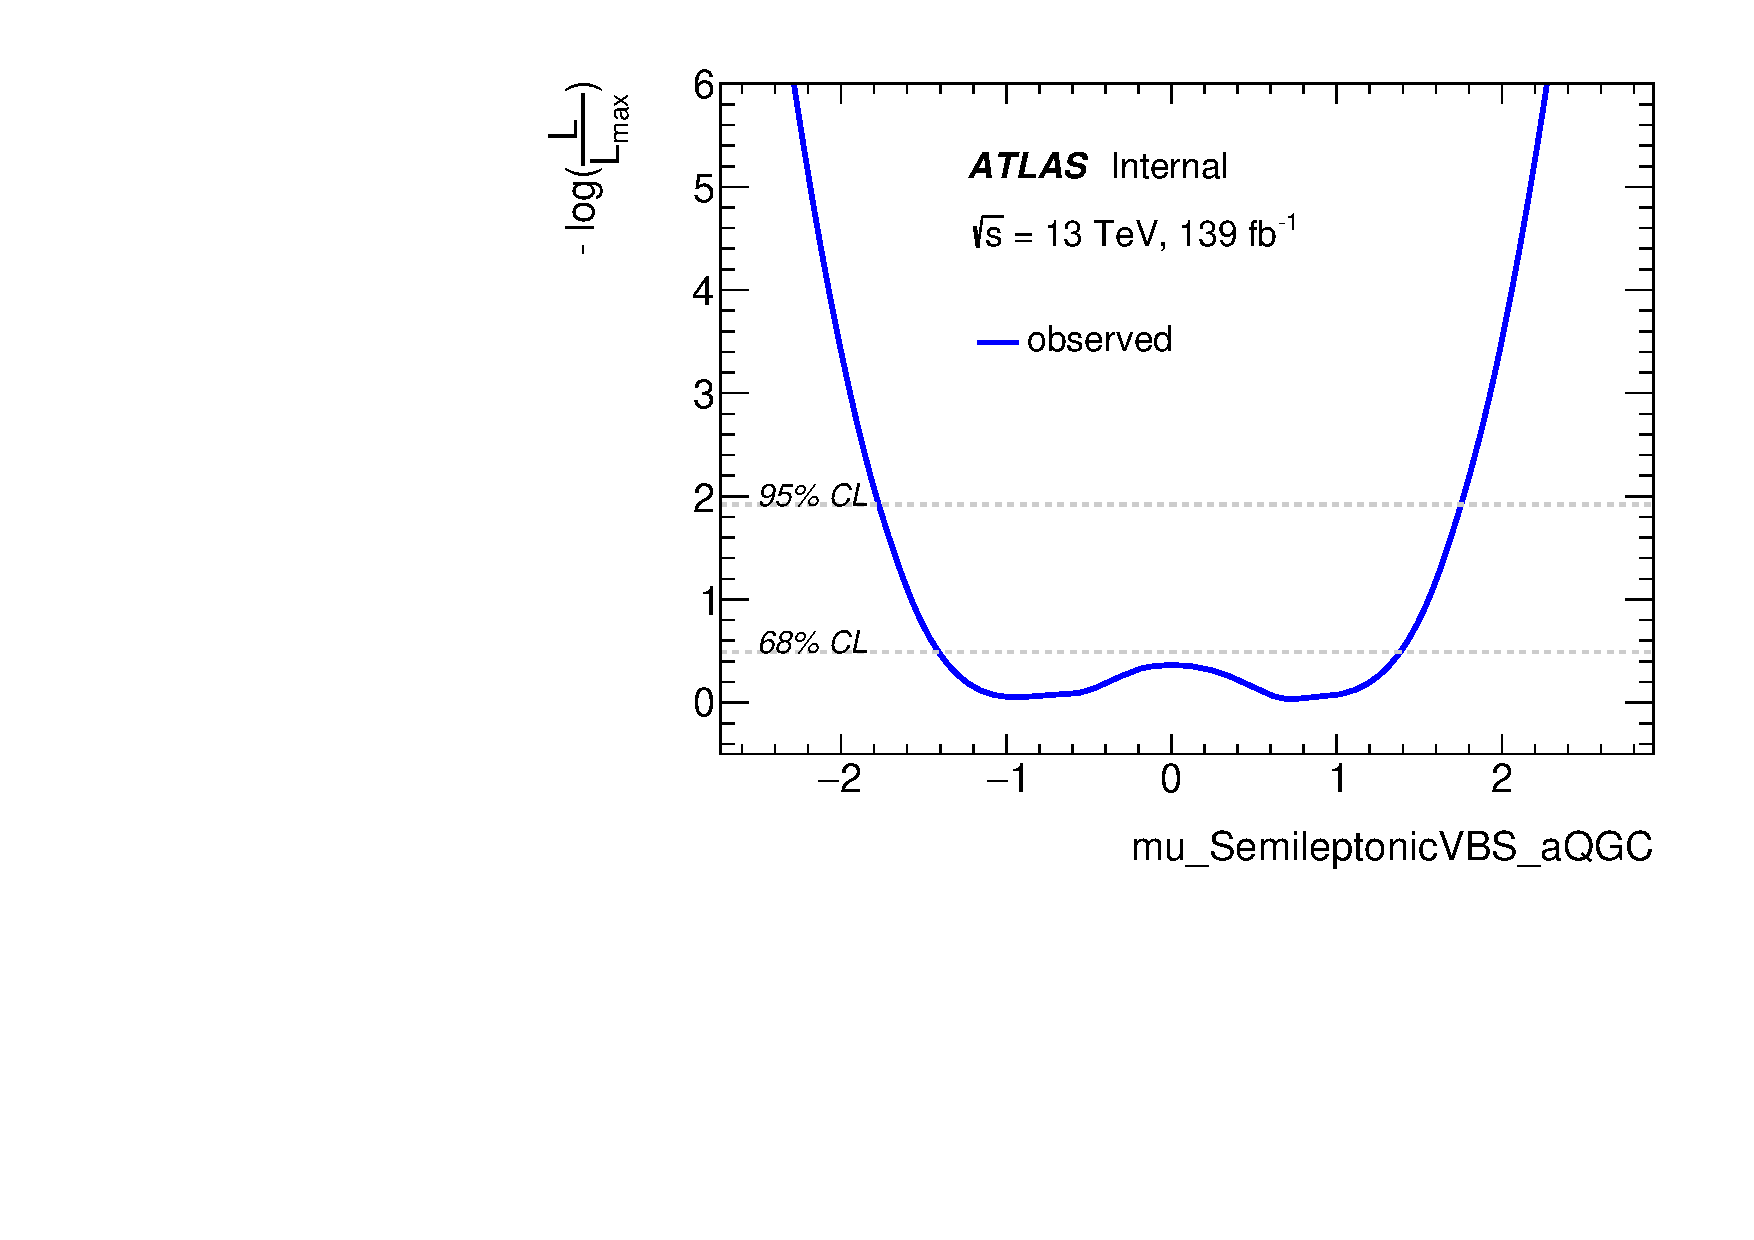
\includegraphics[width=0.38\textwidth]{figures/aQGC/profileFM03000}
        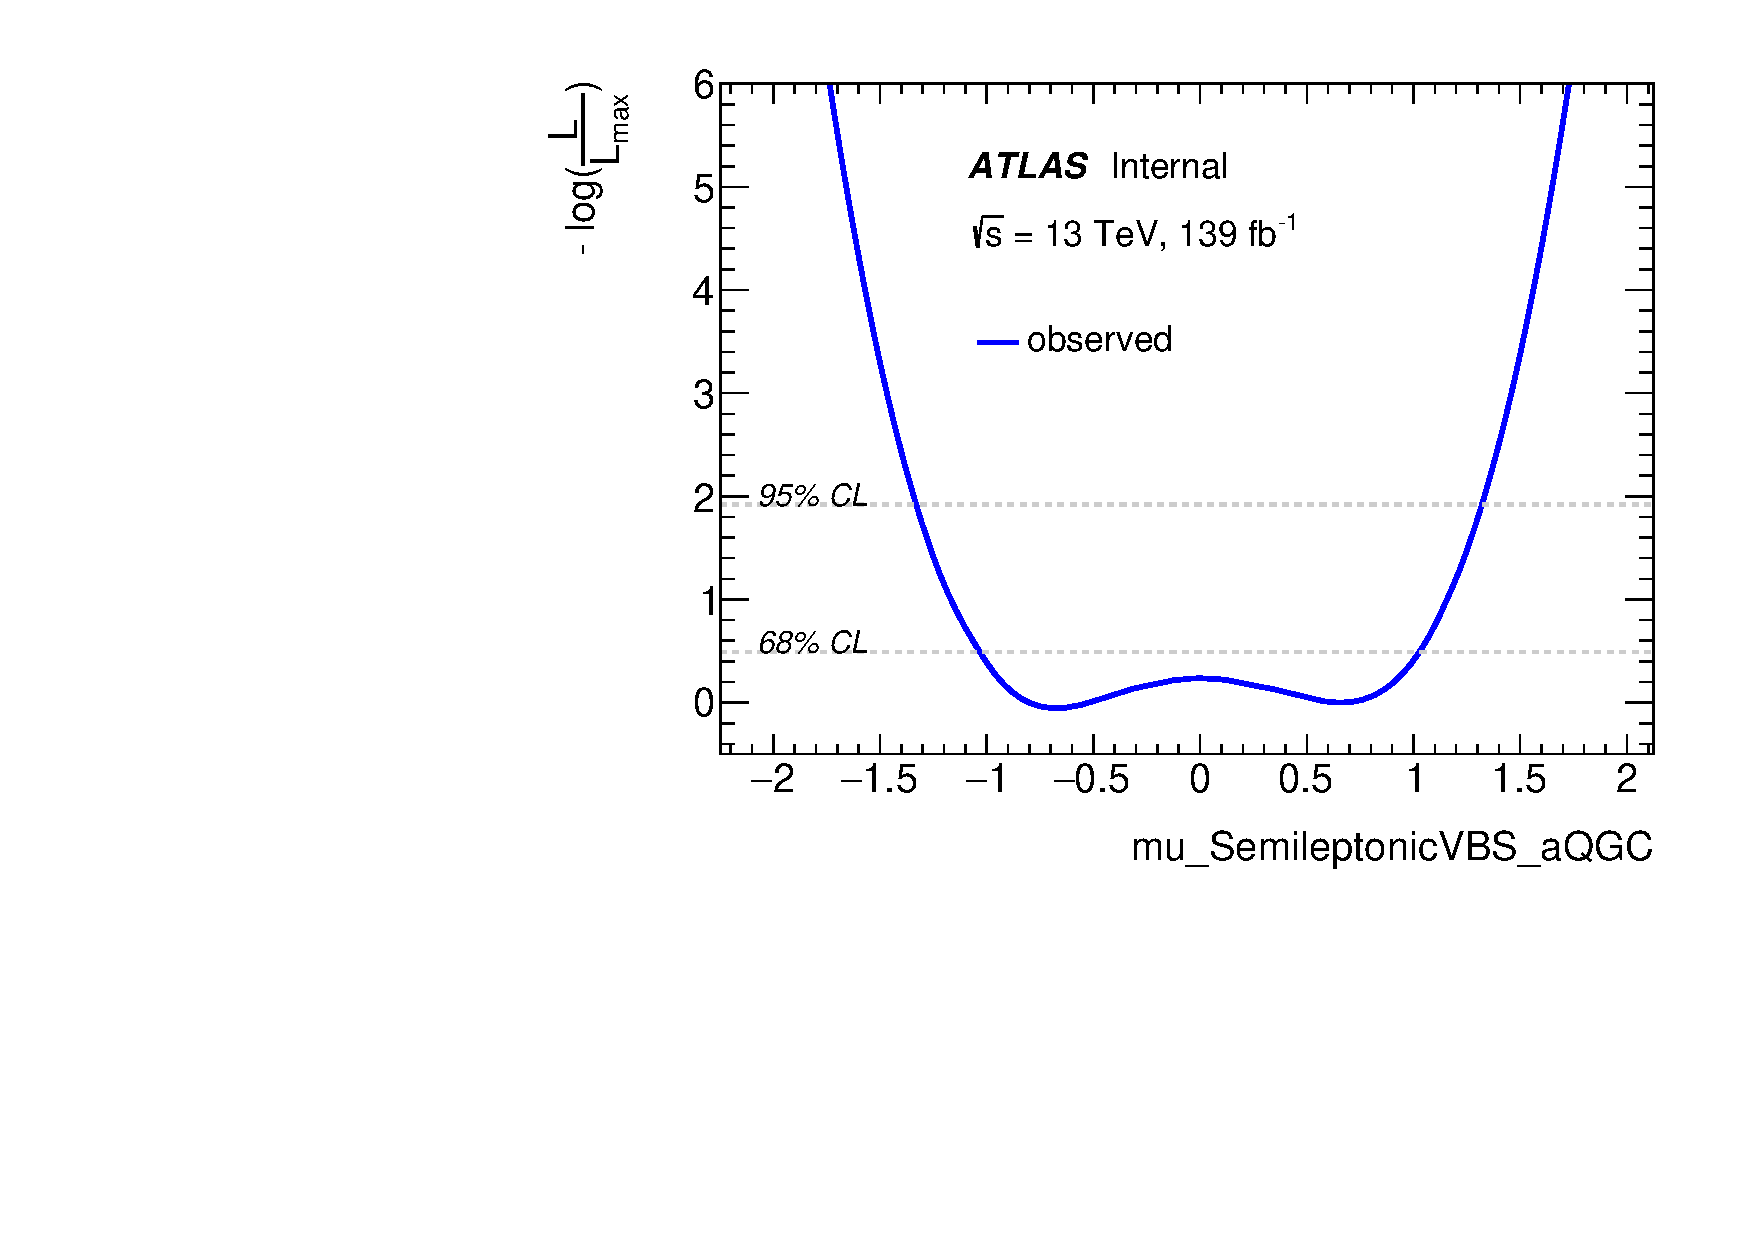
\includegraphics[width=0.32\textwidth]{figures/aQGC/profileFM0inf}
        \caption{The observed log-likelihood curves of FM0 Wilson coefficient where the clipping energy is 1.5~TeV (left), 2.0~TeV (middle), $\infty$ (right).}
        \label{fig:ProfileLLFM}
\end{figure}
%Figure~\ref{fig:QUADINT} shows the distributions of the quardratic term and the interference term for each FT0, FS02, FM0 operator.
%The quardratic term has large contribution compared to the interference term.
Due to the large contribution of the QUAD term in the parametrization of the $\mu_{\mathrm{aQGC}}$, the log-likelihood curve has two local minimums.
A $\mu_{\mathrm{aQGC}}$ value at crossing the 95\% confidence interval line and the likelihood curve is used to calculate upper and lower limits on the coefficients. 
%The 95\% confidence interval corresponds to 1.9.
For high clipping values, the results exclude the signal strength already excluded by the theoretical unitarity bound.
Table~\ref{tab:aQGClimits} shows the uniterized and ununiterized expected and observed limits from figure~\ref{fig:aQGClimits}, where uniterized limit is the intersection point of the theoretical unitality bound and experimental limit line, while ununiterized limit is the limit with no clipping energy.
\begin{figure}[ht]
    \centering
    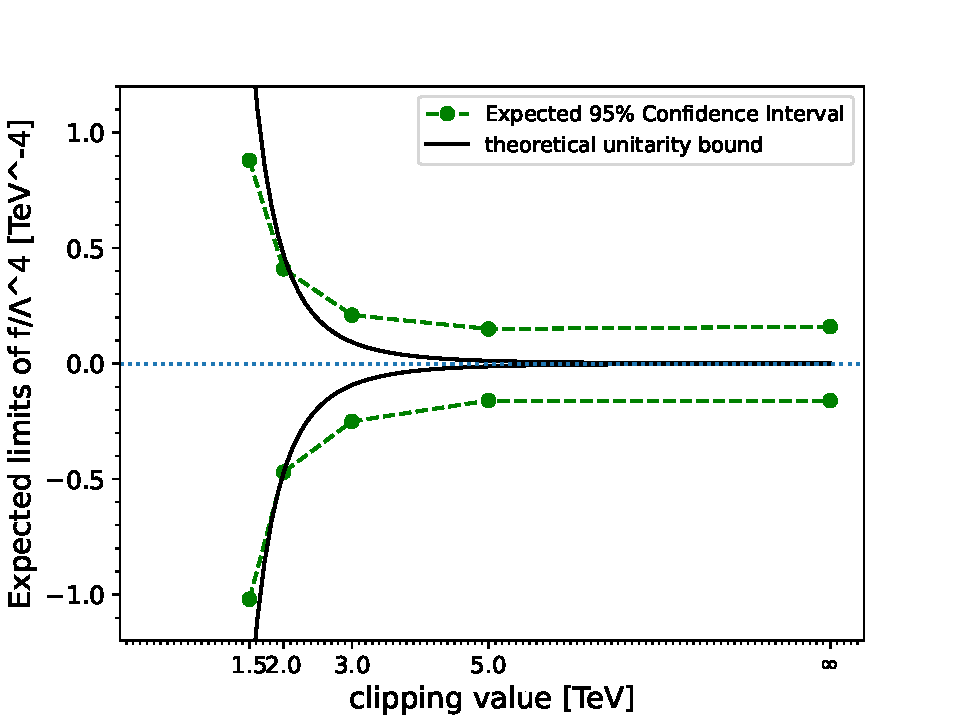
\includegraphics[width=0.45\textwidth]{figures/aQGC/ClippedFT0CI.pdf}
    	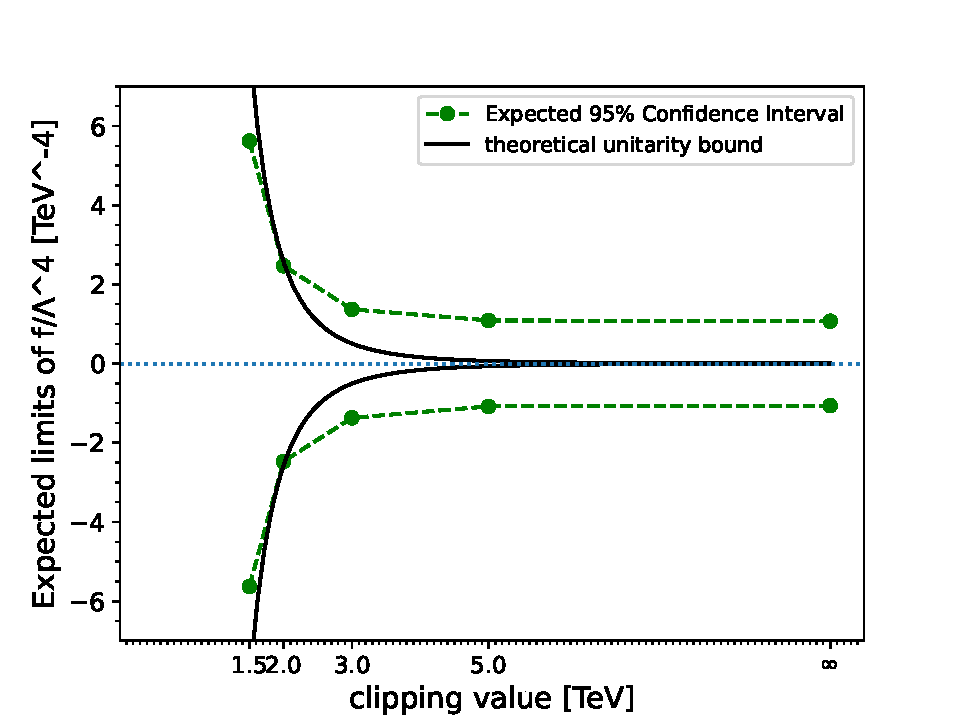
\includegraphics[width=0.45\textwidth]{figures/aQGC/ClippedFM0CI.pdf}
    	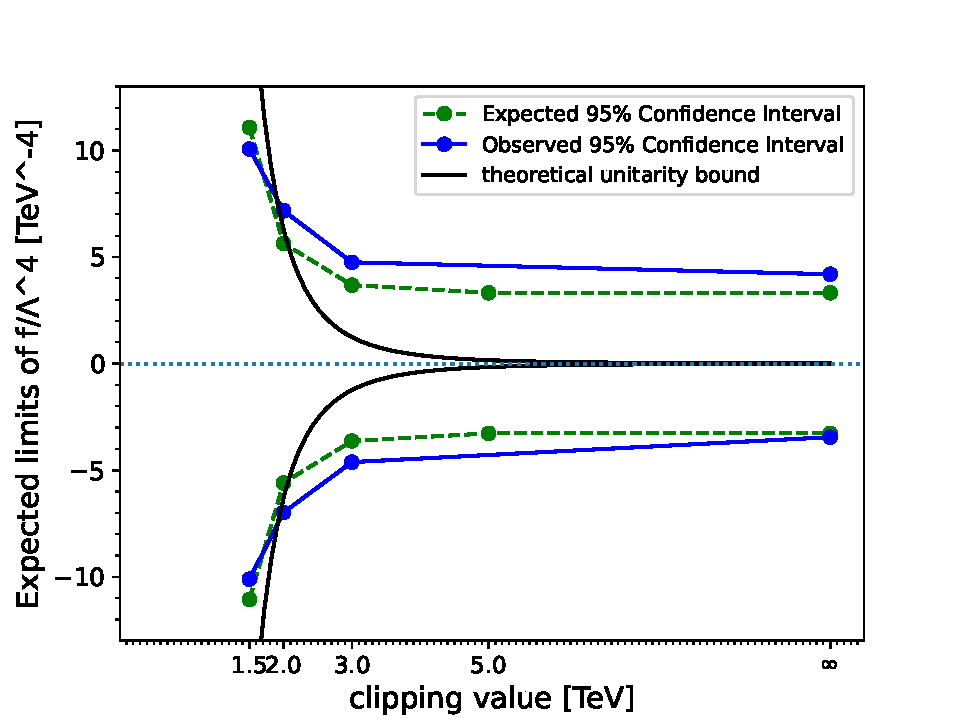
\includegraphics[width=0.45\textwidth]{figures/aQGC/ClippedFS02CI.pdf}
        \caption{Expected limits (green) and observed limits (blue) for 5 clipping points are shown for each Wilson coefficient FT0 (left), FM0 (right), FS02 (middle). The black line is the theoretical unitarity bound.}
        \label{fig:aQGClimits}
\end{figure}

%\begin{table}[ht!]
%\small
%\begin{center}
%%\resizebox{0.9\textwidth}{!}{
%\begin{tabular}{ | l || l | l | l | l | l |}
%\hline
%                   & 1.5 [ TeV ] & 2.0 [ TeV ] & 3.0 [ TeV ] & 5.0 [ TeV ] & $\infty$                  \tabularnewline \hline
%FT0                & [ -1.02, 0.88 ]  & [ -0.47, 0.41 ]  & [ -0.25, 0.21 ]  & [ -0.16, 0.15 ]  & [ -0.16, 0.16 ]              \tabularnewline \hline
%FM0                & [ -5.63, 5.62 ]  & [ -2.47, 2.47 ]  & [ -1.37, 1.37 ]  & [ -1.08, 1.09 ]  & [ -1.06, 1.07 ]              \tabularnewline \hline

%\caption{Expected limits for each clipping point. Ununiterized limit is shown as the limit with no clipping energy, labeled as $\infty$ in figure~\ref{fig:aQGClimits}.}
%\label{tab:aQGClimits}
%\end{center}
%\end{table}

%uniterized limit
\begin{table}[ht!]
\small
\begin{center}
\resizebox{0.9\textwidth}{!}{
\begin{tabular}{ | l || l | l | l | l | }
\hline
                   & \multicolumn{2}{|l|}{expected limit}                           & \multicolumn{2}{|l|}{observed limit} \tabularnewline \hline
Wilson coefficient & uniterized                  & ununiterized               & uniterized                     & ununiterized \tabularnewline \hline
FT0                &  [ -0.48, 0.39 ] at [ 1.99, 2.09 ]~TeV           & [ -0.16, 0.16 ]            & [ -1.04, 0.74 ] at [ 1.64, 1.78 ]~TeV & [ -0.25, 0.23 ]\tabularnewline \hline
FM0                &  [ -2.99, 2.97 ] at [ 1.92, 1.92 ]~TeV           & [ -1.06, 1.07 ]            & [ -1.63, 1.63 ] at [ 2.24, 2.24 ]~TeV & [ -1.32, 1.31 ]\tabularnewline \hline
FS02               &  [ -5.46, 5.61 ] at [ 2.05, 2.07 ]~TeV           & [ -3.27, 3.32 ]            & [ -7.53, 7.80 ] at [ 1.91, 1.90 ]~TeV & [ -3,45, 4.19 ]\tabularnewline \hline
\end{tabular}
}
\caption{Uniterized and ununiterized expected limits and observed limits. Uniterized limit is the intersection point of the theoretical unitality bound and experimental limit line. Ununiterized limit is the limit with no clipping energy, labeled as $\infty$ in figure~\ref{fig:aQGClimits}.}
\label{tab:aQGClimits}
\end{center}
\end{table}

%The same procedure is performed with all 17 Wilson coefficient.
%The uniterized expected limit and the ununiterized expected limit is plotted in figure~\ref{}.


